\documentclass[../main.tex]{subfiles}
\begin{document}
\chapter{Resultados}
A continuación se reportan los resultados obtenidos con la metodología descrita en el capítulo anterior.
\section{Muestras Sintetizadas} \label{sec:sintesis}
Se sintetizaron un total de 8 muestras de 1g, 4 de \neod{} y 4 de \sama{} respectivamente. Una muestra de cada una fue reservada para realizar un análisis termogravimétrico. A través de éste, se determinó la temperatura mínima de calcinación para ambas ortoferritas, como se reporta en la sección \ref{sec:TGA}.

Con estas temperaturas como punto de partida, 600\gradoC{} para el \neod{} y 700\gradoC{} para el \sama{}, se calcinaron el resto de muestras, 4 muestras de \neod{} se calcinaron a 600\gradoC{}, para las otras 3 se aumentó la temperatura 100\gradoC{} por cada una, es decir, se calcinaron a 700, 800 y 900\gradoC{} respectivamente.

Por otro lado, para el \sama{} se calcinaron 4 muestras a 700\gradoC{}, aumentando la temperatura de la misma forma que en el caso del \neod{} para las otras 3, es decir, se calcinaron a 800, 900 y 1000\gradoC{} respectivamente.

En ambos casos se obtuvieron polvos de color café rojizo con apariencia porosa, como se muestra en la figura \ref{fig:resfotomuestra}.
\begin{figure}[H]
    \centering
    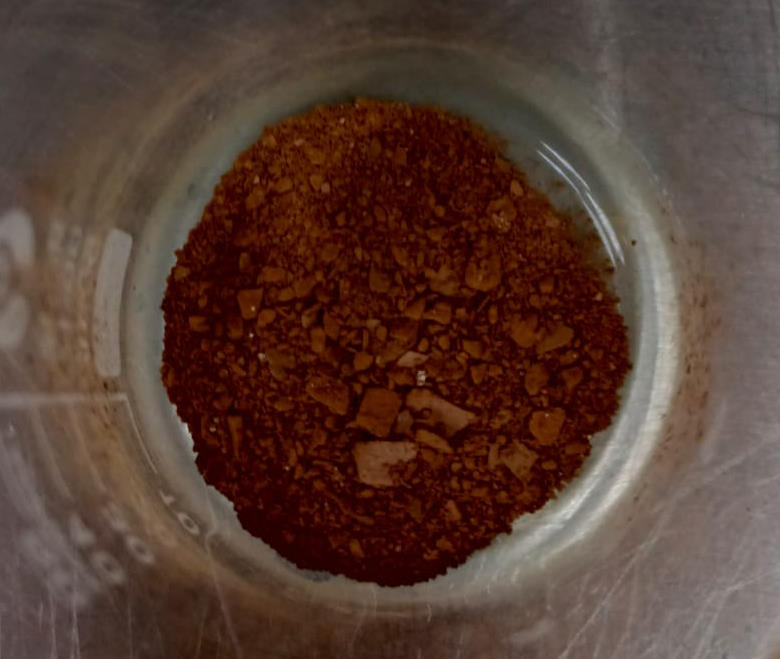
\includegraphics[width=0.45\textwidth]{fig/muestraSmFeO3900.jpeg}
    \caption{Muestra de \sama{} calcinada a 900\gradoC.}
    \label{fig:resfotomuestra}
\end{figure}
\section{Caracterización estructural y morfológica}
En esta sección se reportan los resultados obtenidos a través de las técnicas descritas en el capítulo \ref{cap:metodologia}.
\subsection{Análisis Termogravimétrico} \label{sec:TGA}
Se realizó un análisis termogravimétrico a ambas ortoferritas. Se obtuvieron las curvas de peso contra temperatura que me muestran en la figura \ref{fig:TGAres} (a) y (b) para \neod{} y \sama{} respectivamente:
\begin{figure}[H]
    \centering
    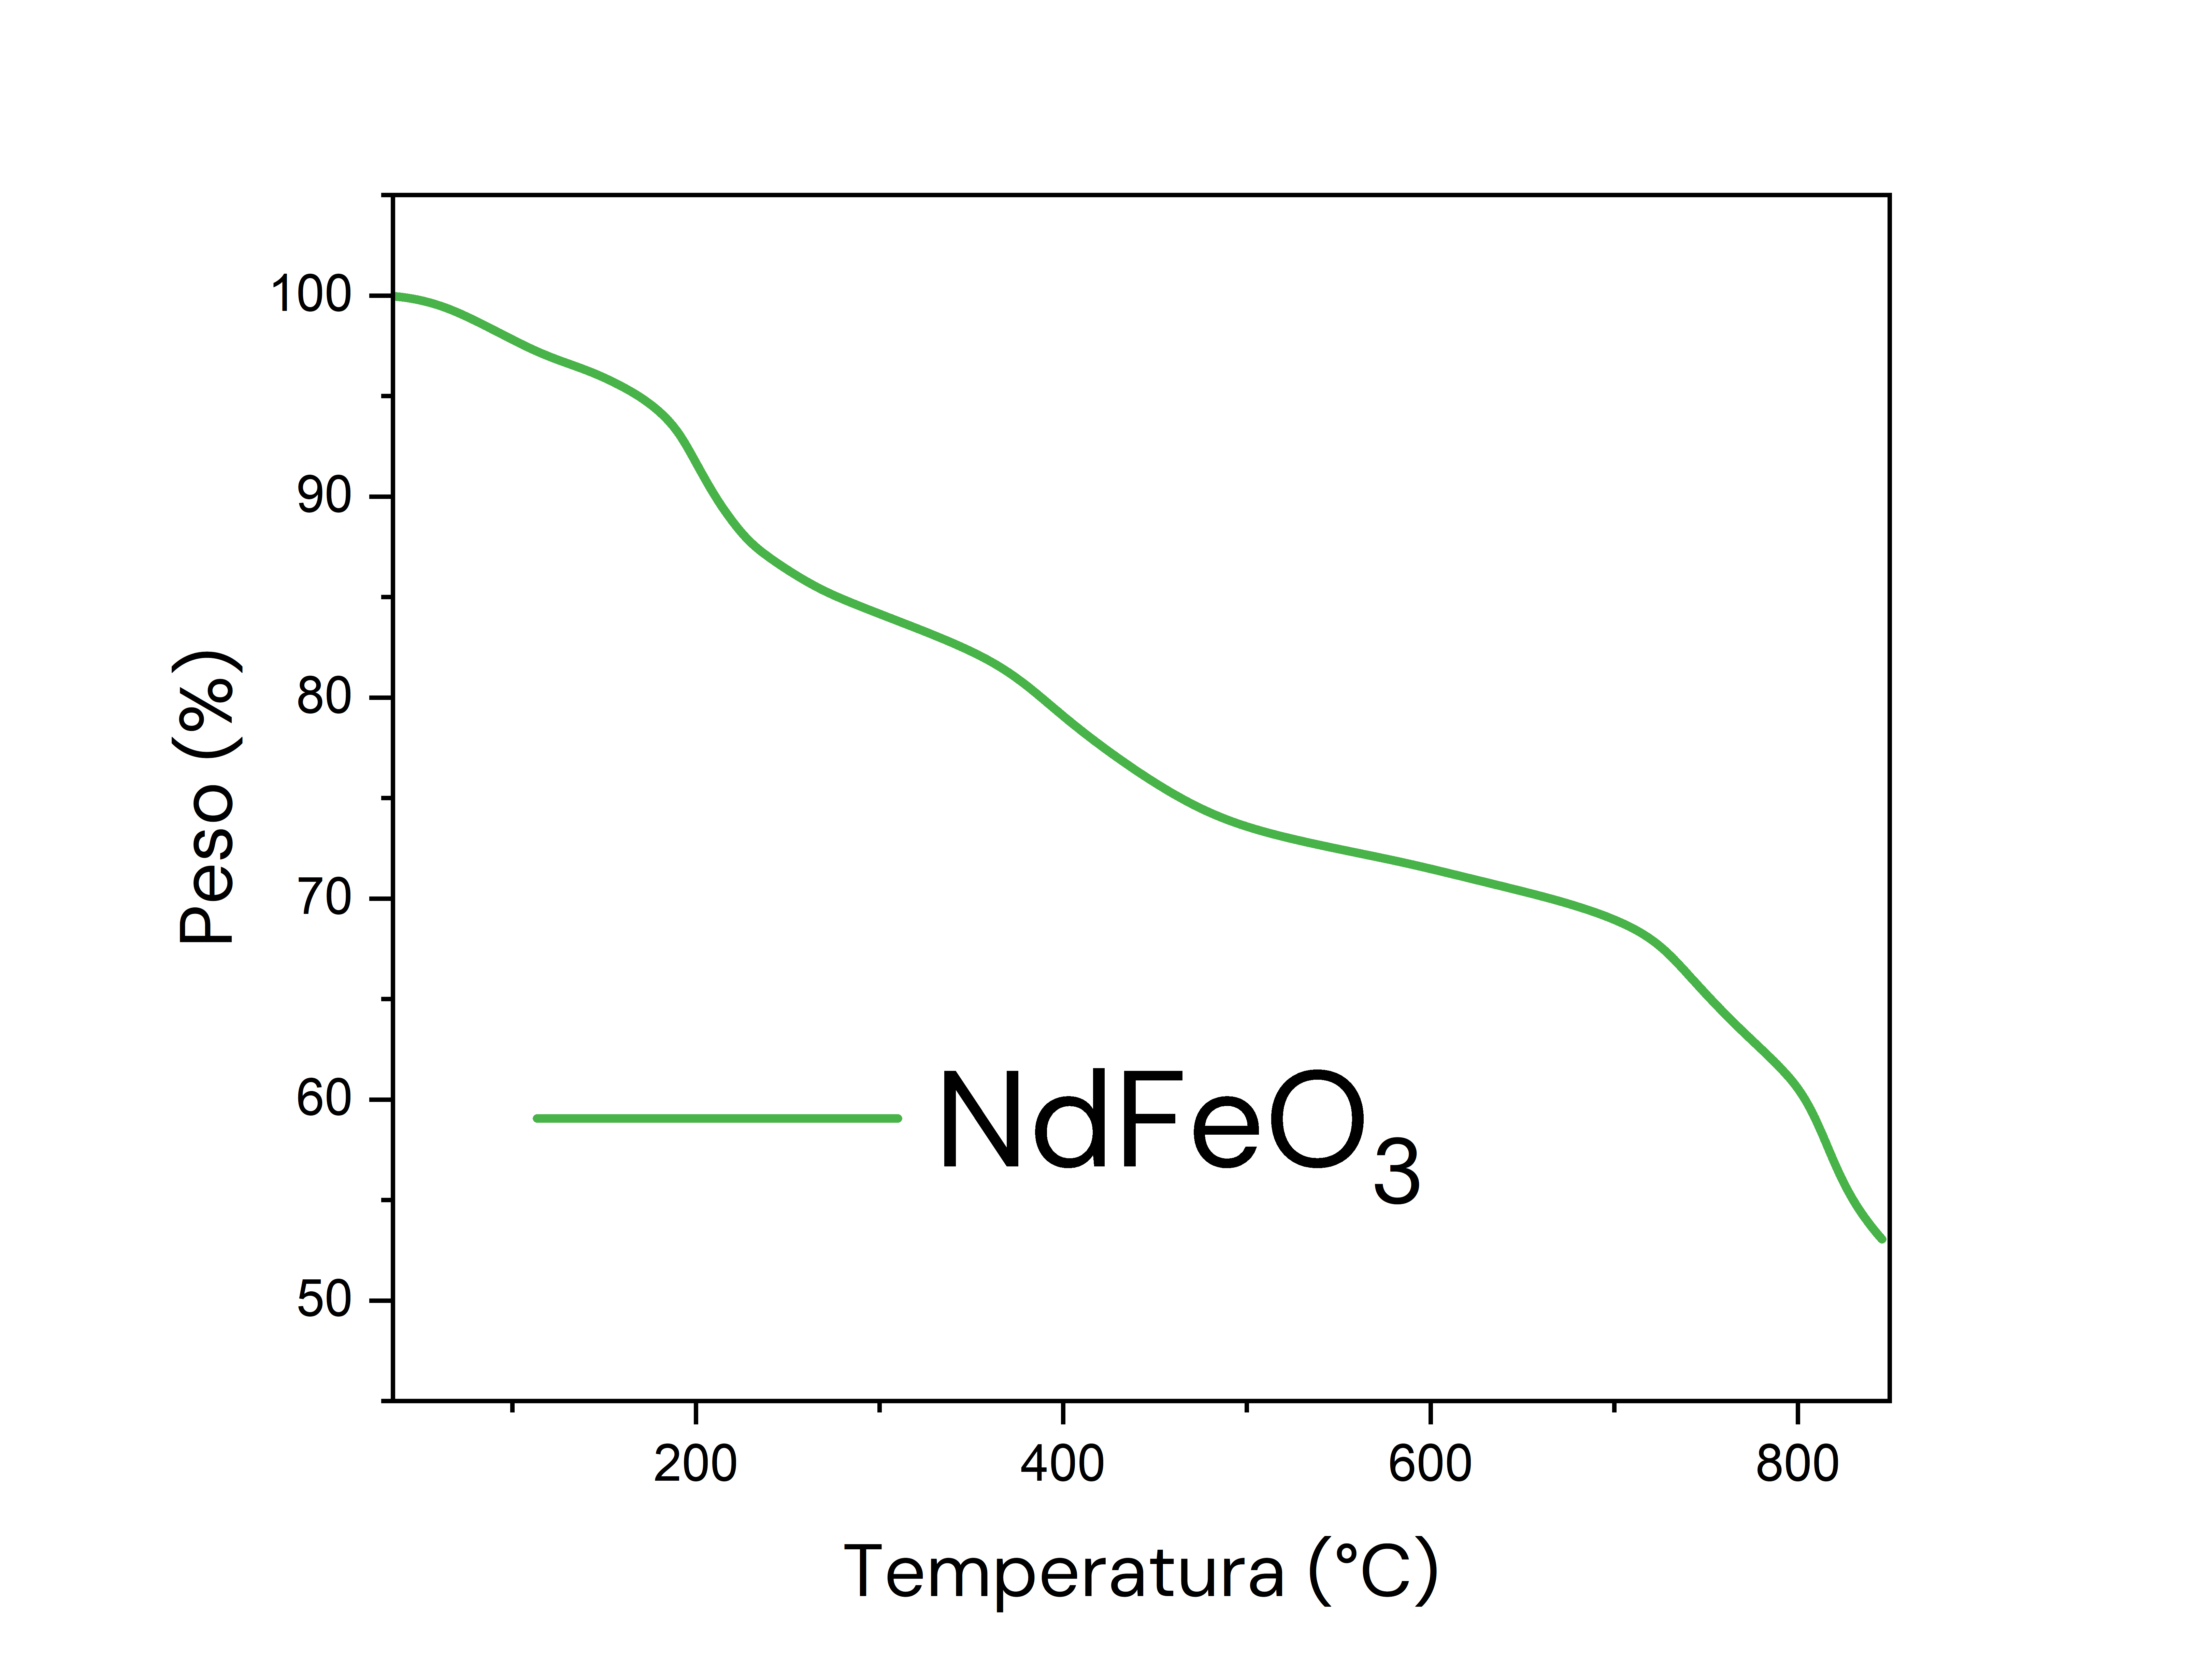
\includegraphics[width=0.4\textwidth]{fig/TGA-NdFeO3.png}
    \quad
    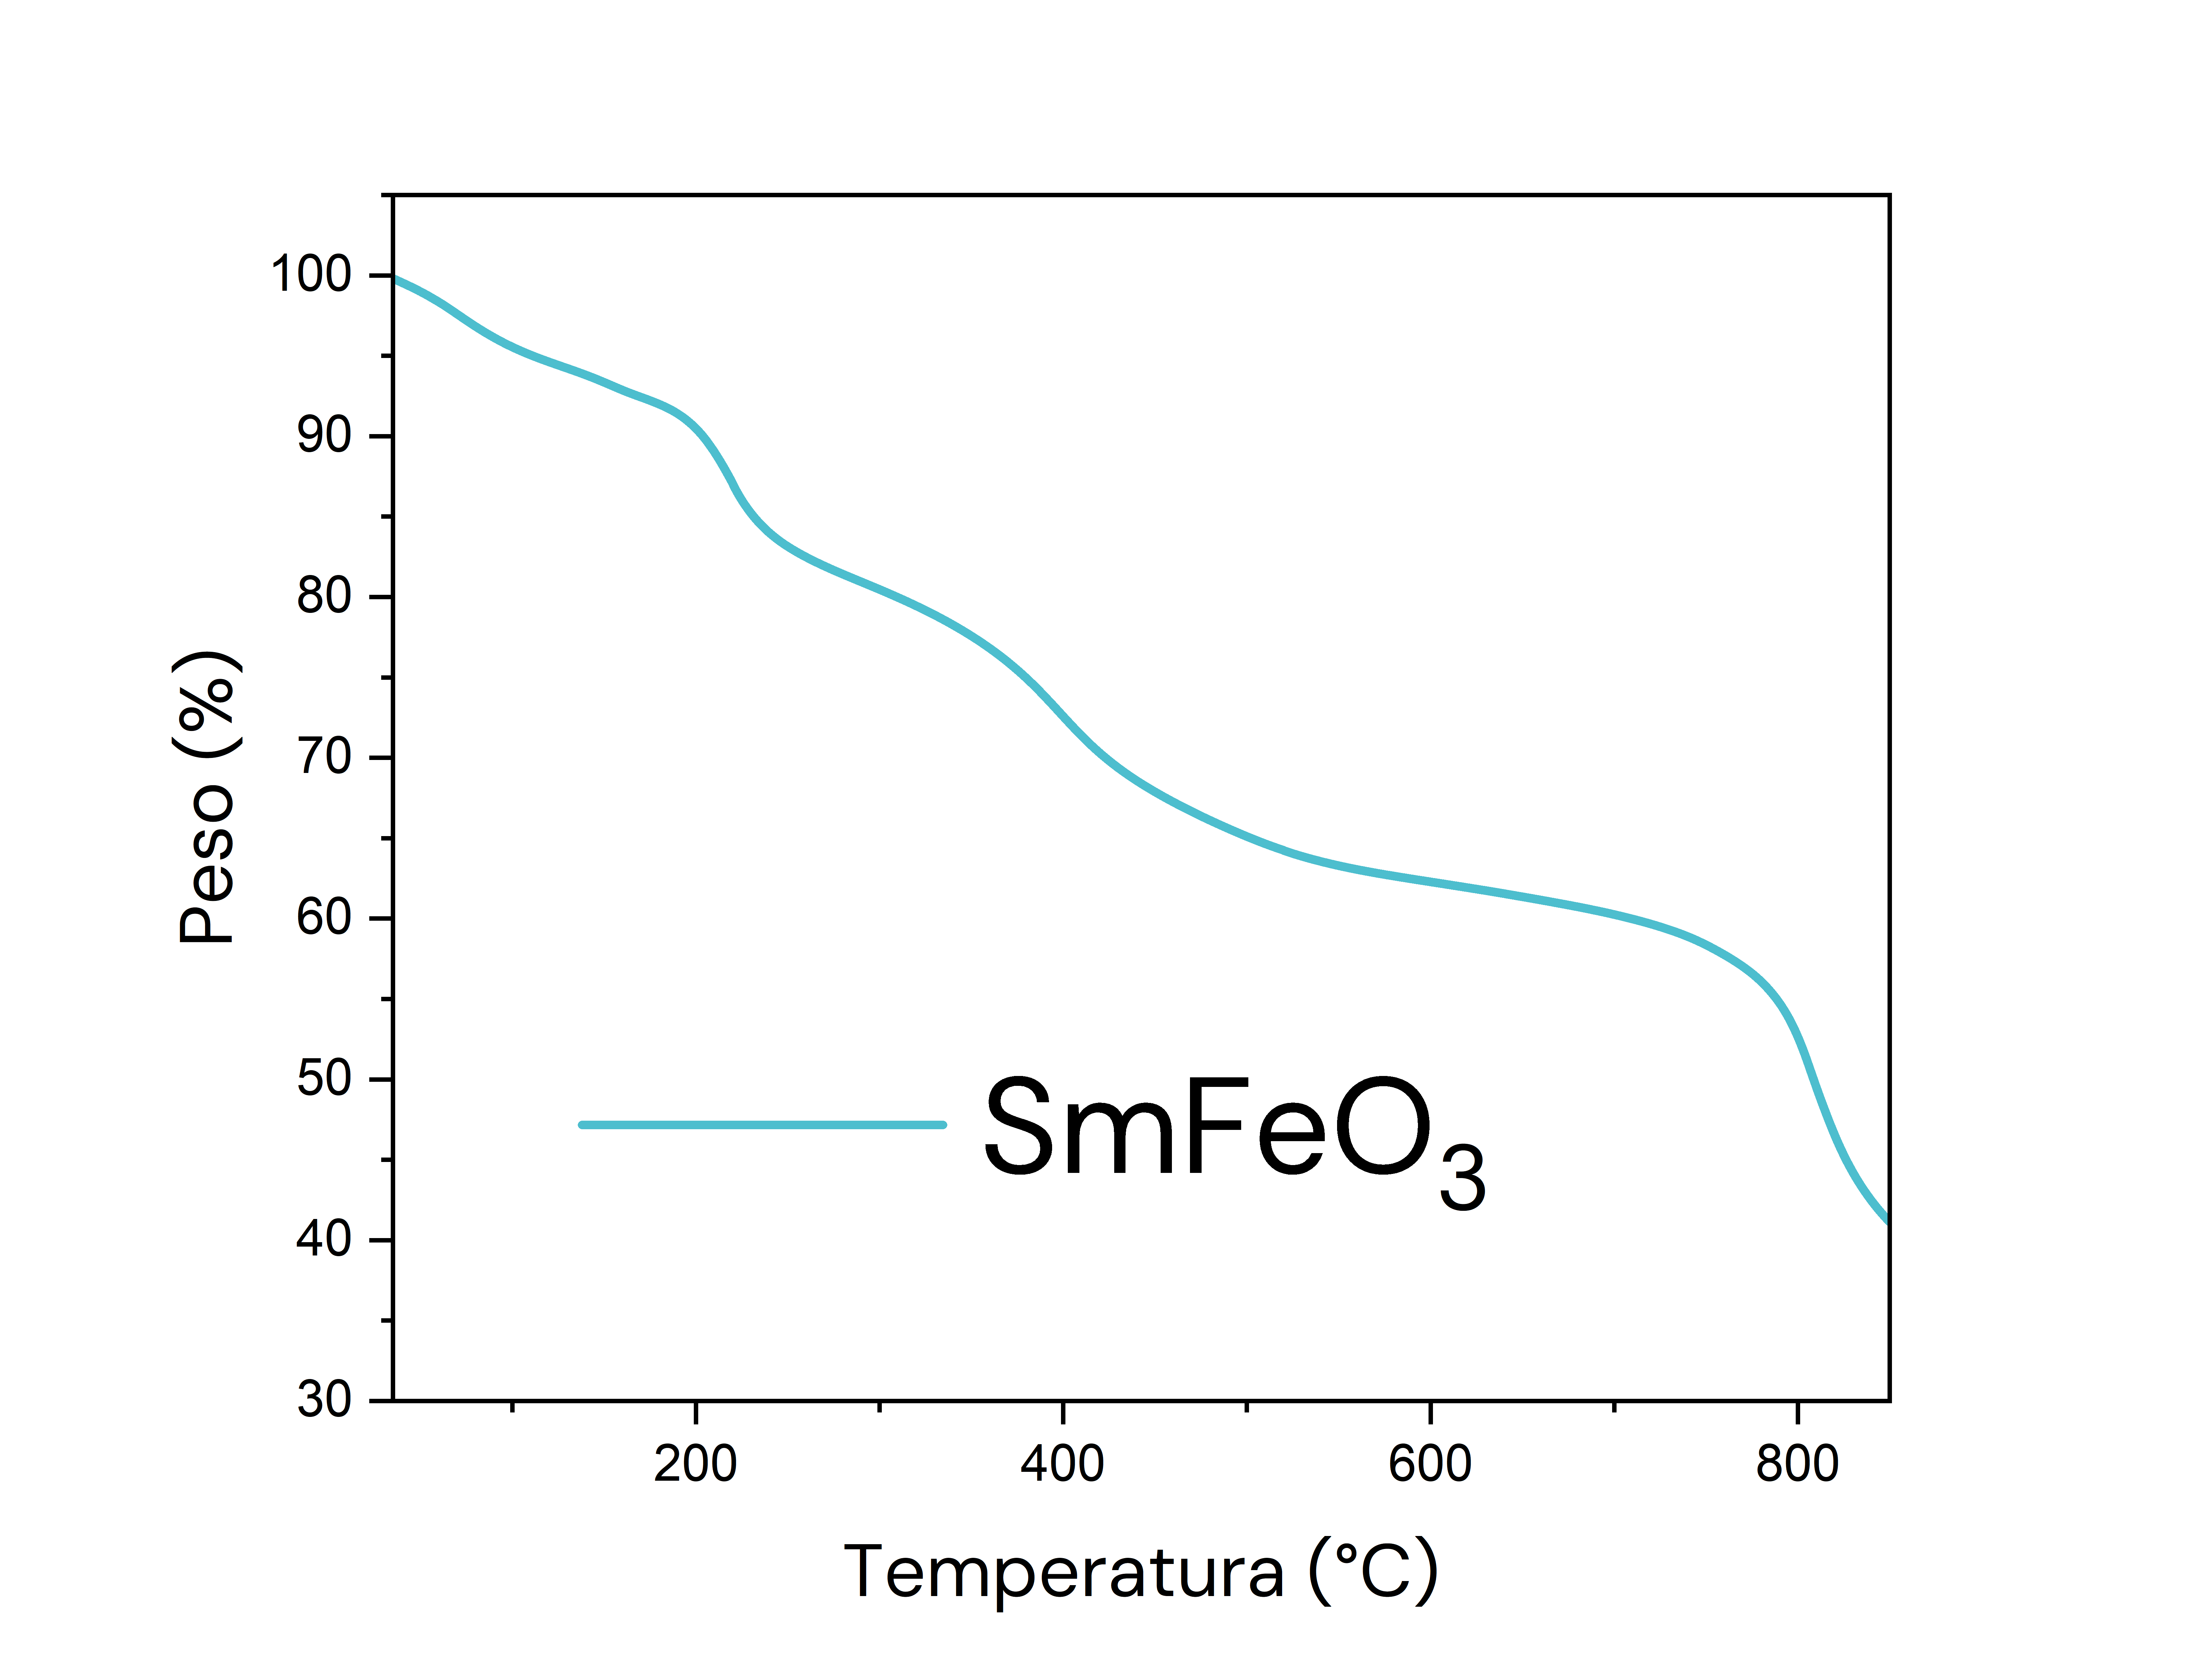
\includegraphics[width=0.4\textwidth]{fig/TGA-SmFeO3.png}
    \caption{Análisis termogravimétrico de las ortoferritas. a) \neod{}, b) \sama{}}
    \label{fig:TGAres}
\end{figure}
Al obtener la derivada del peso respecto a la temperatura se obtuvieron las curvas que se muestran en la figura \ref{fig:derTGAres}:
\begin{figure}[H]
    \centering
    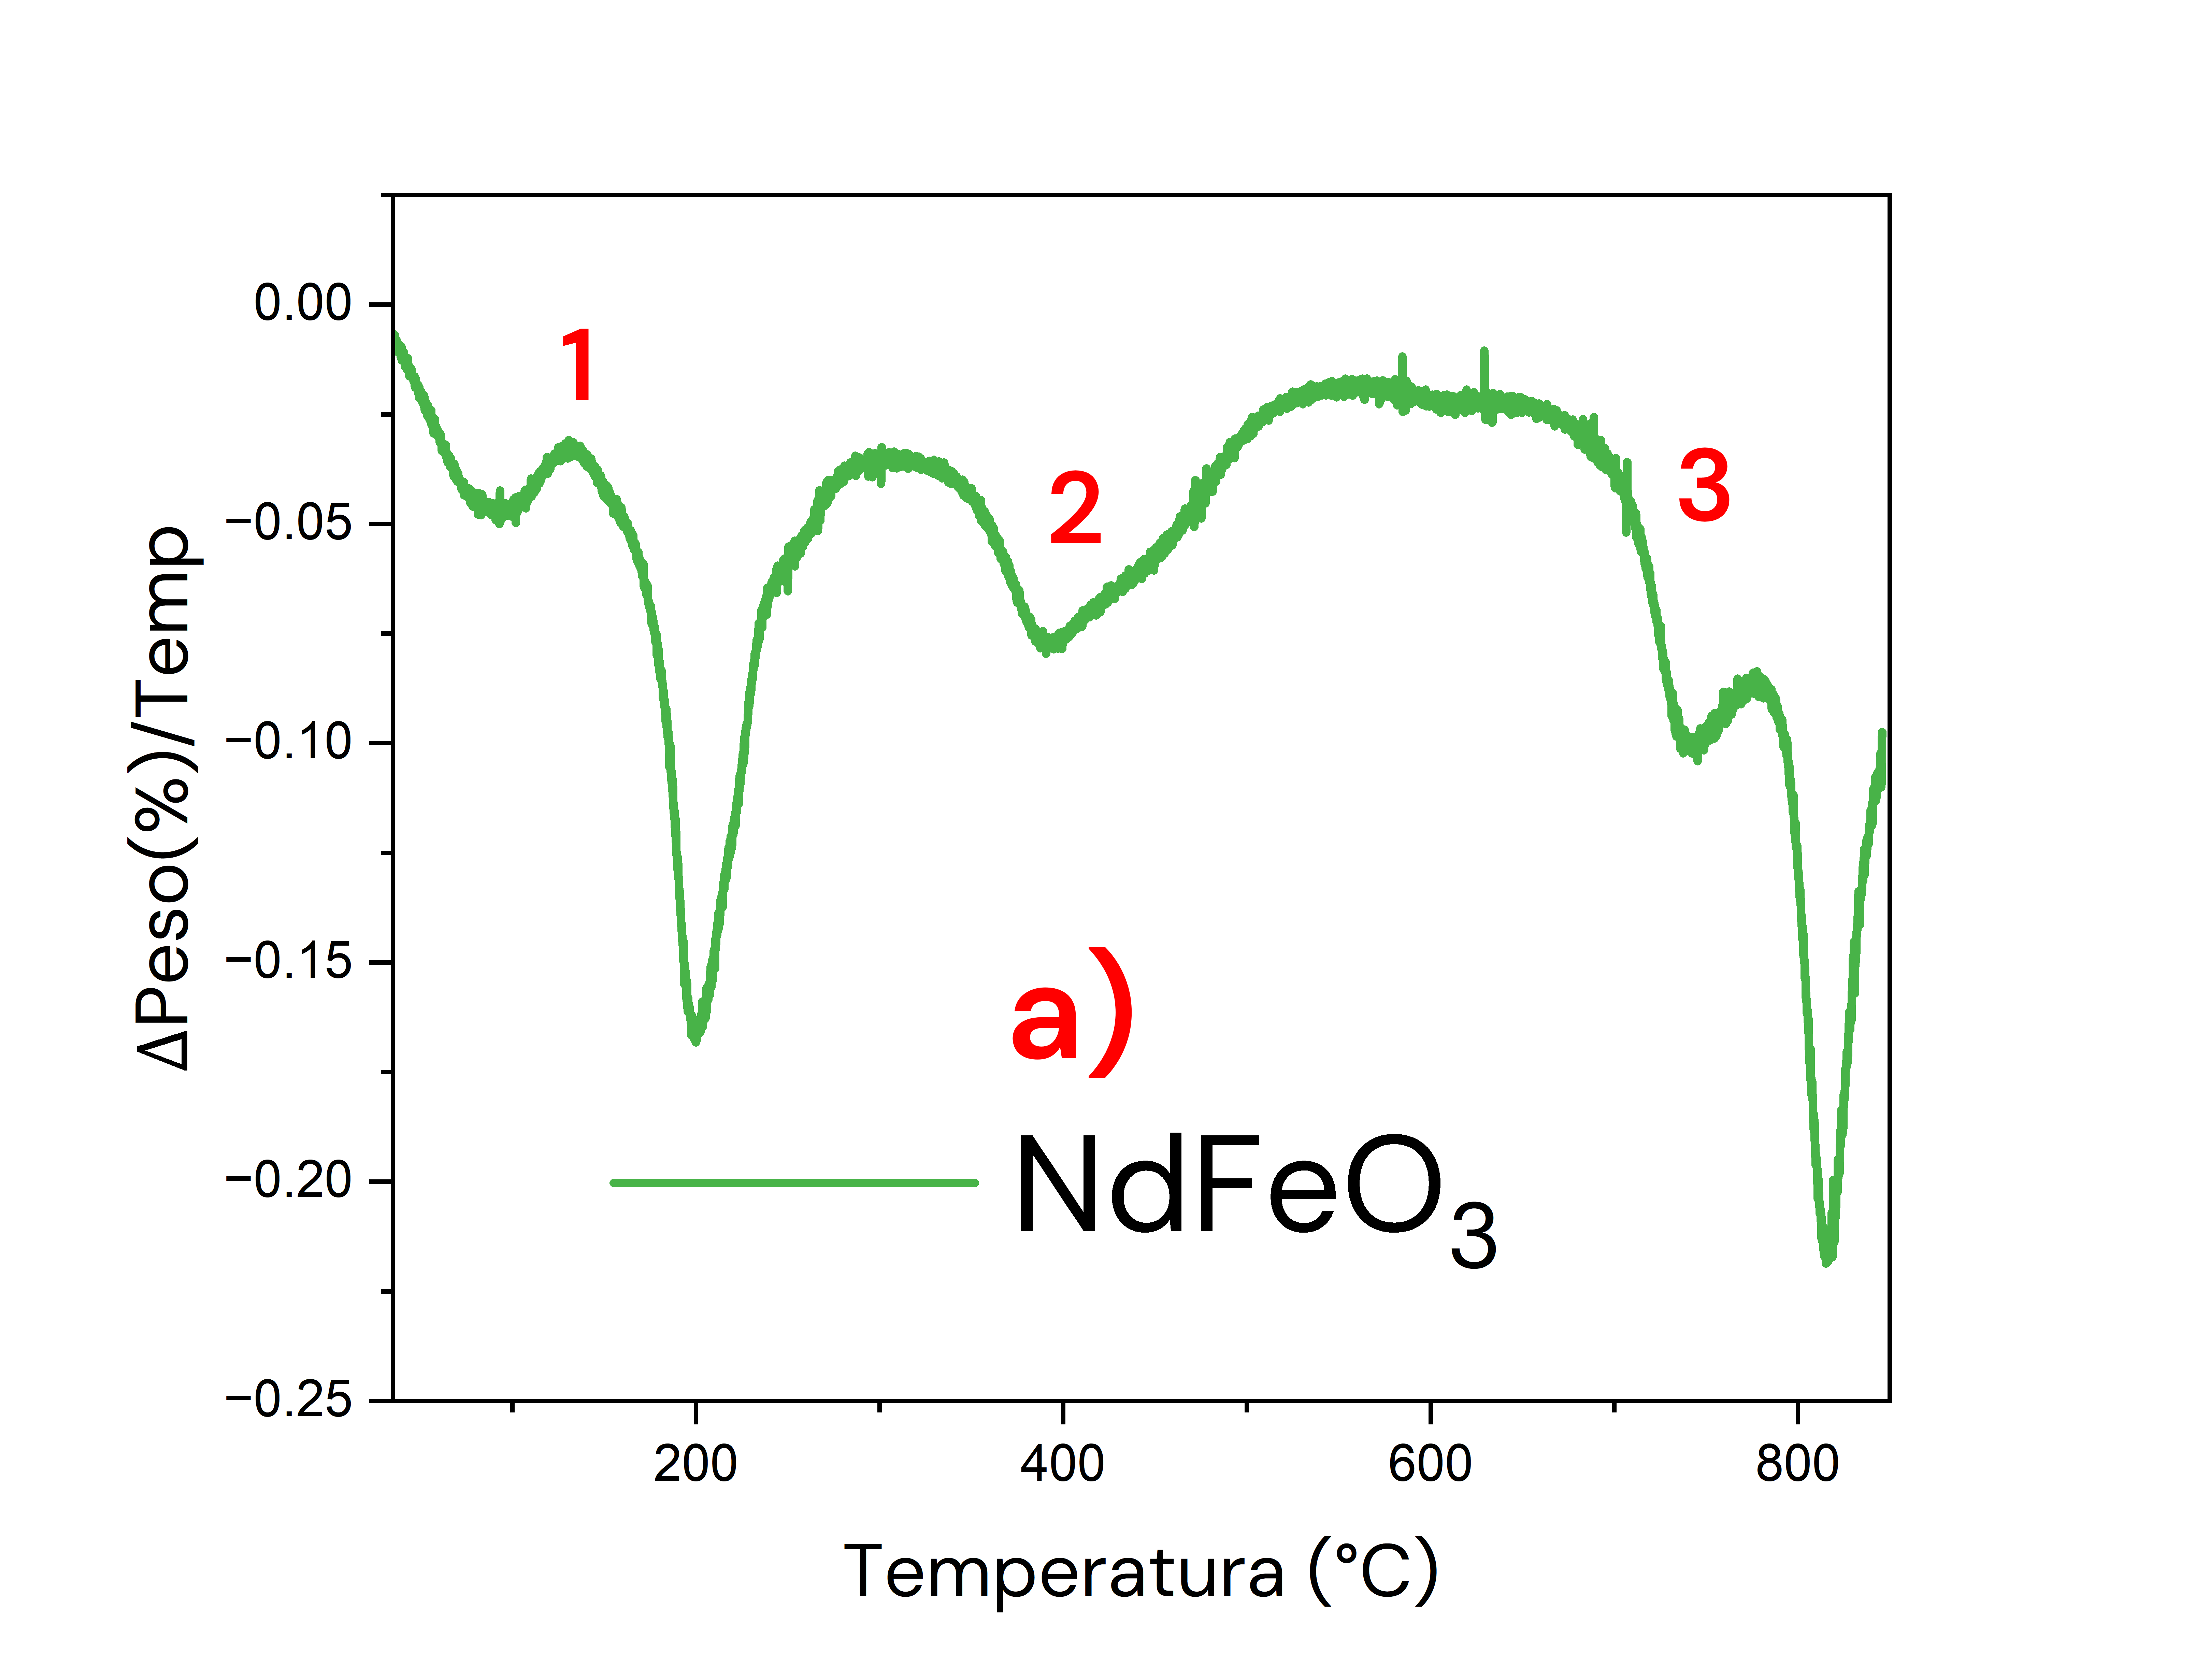
\includegraphics[width=0.4\textwidth]{fig/TGA-derNdFeO3.png}
    \quad
    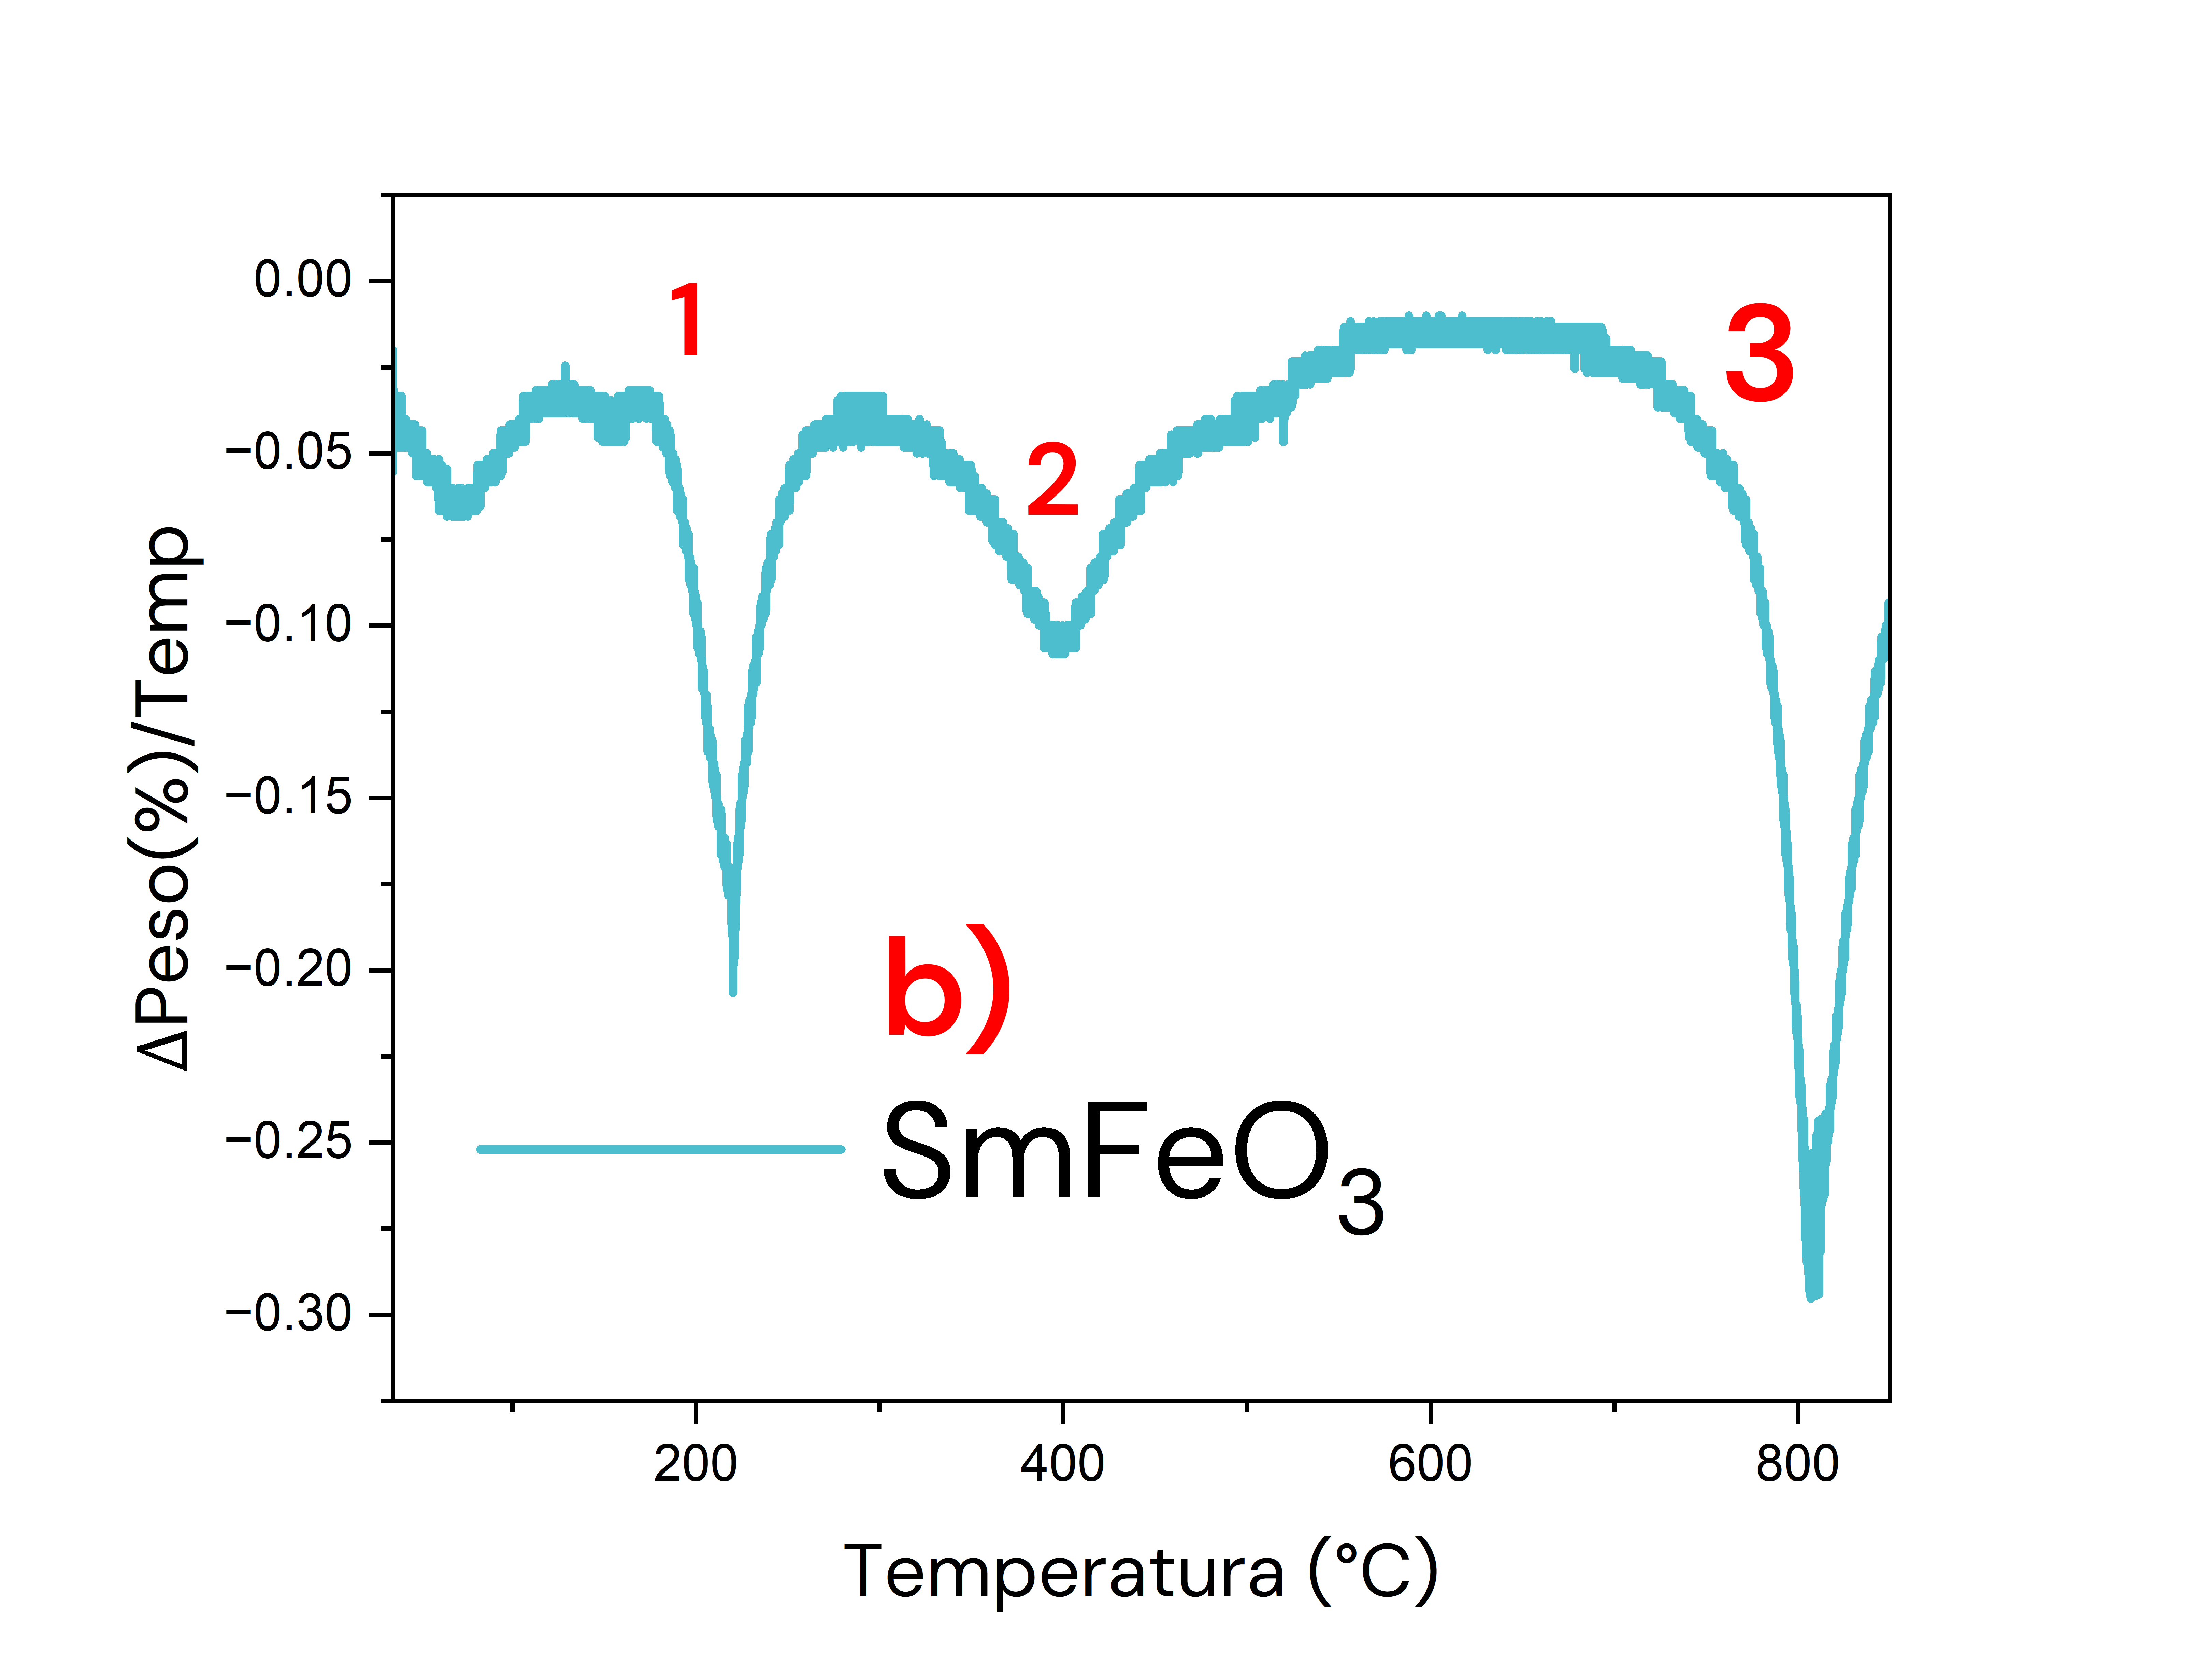
\includegraphics[width=0.4\textwidth]{fig/TGA-derSmFeO3.png}
    \caption{Derivada de la masa respecto a la temperatura para ambas ferritas. a) \neod{}, b) \sama{}}
    \label{fig:derTGAres}
\end{figure}
Se pueden observar 3 regiones distintas donde ocurren cambios térmicos en la muestra:
\begin{table}[H]
    \centering
    \begin{tabular}{|c|c|}
        \hline
        Zona & Temperatura\\
        & aproximada\\\hline\hline
        1&100-200\gradoC{}\\
        \hline
        2&300-500\gradoC\\\hline
        3&>700\gradoC\\
        \hline
    \end{tabular}
    \caption{Regiones donde cambia el comportamiento de la masa respecto a la temperatura para ambas muestras.}
    \label{tabla:TGAtabla}
\end{table}
La región 1 coincide con las temperaturas a la que el agua se evapora y se combustiona la fase orgánica en la muestra.

De acuerdo a lo reportado en la literatura \cite{Navarro2005} \cite{Yadav2023}, la formación de la fase cristalina ocurre entre 600-1000 °C, siendo esta temperatura muy sensible al método y las condiciones de síntesis.

Se piensa que en la región 2 comienza la cristalización de las ortoferritas, mientras que en la región 3 ocurre un crecimiento de los cristales, de acuerdo con las observaciones que se discutirán en la sección \ref{sec:resrietlveld}.
\subsection{Microscopía electrónica de barrido}
Se estudió la morfología de las partículas sintetizadas a través de esta técnica, dando como resultado imágenes como las que se muestran en las figuras \ref{fig:resSEM900}-\ref{fig:resSEMsonicada4}.
\begin{figure}[H]
    \centering
    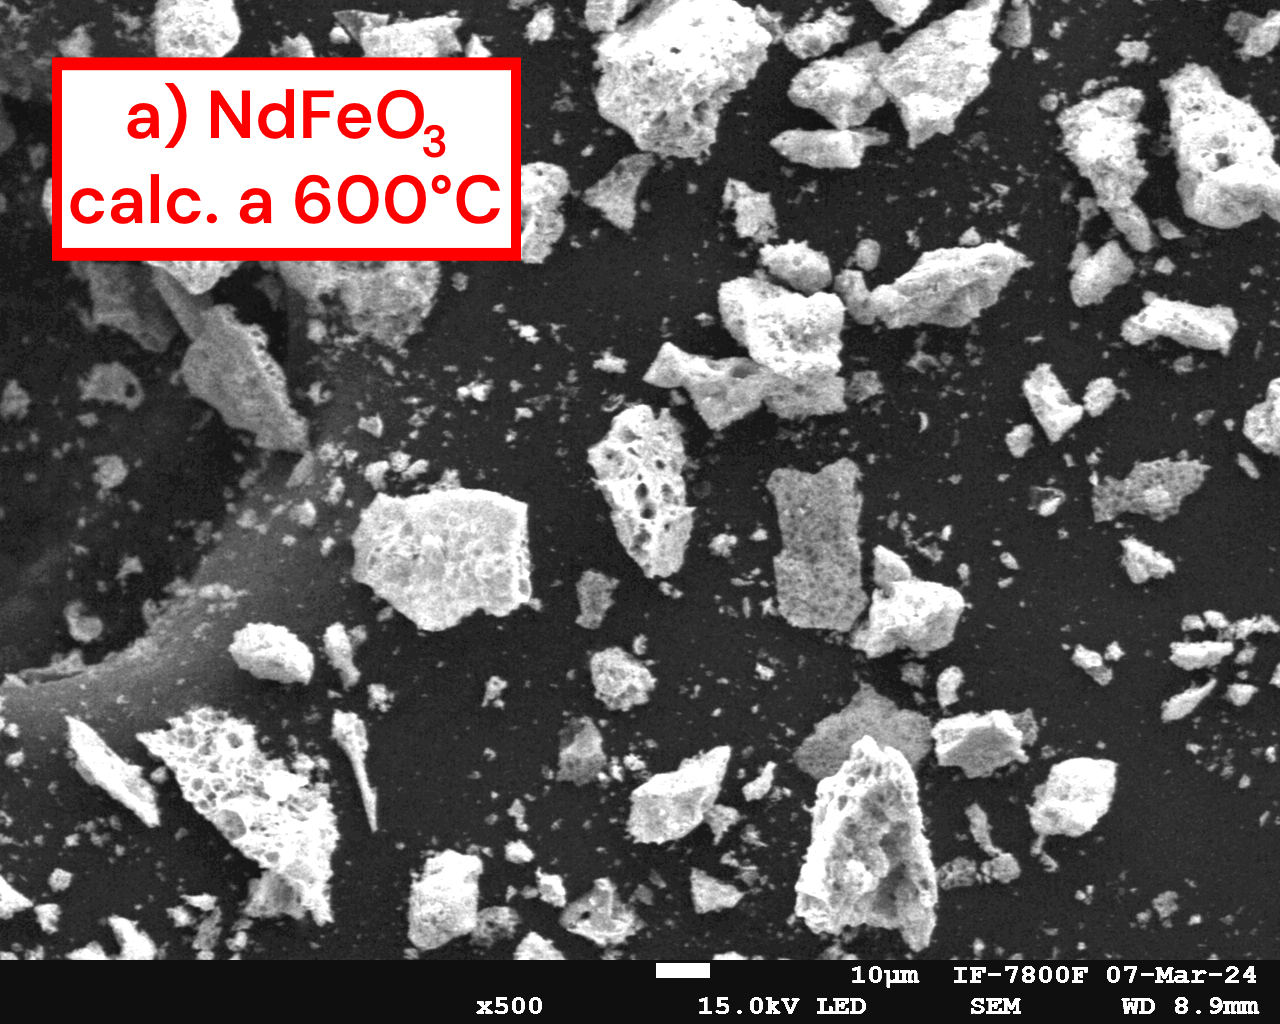
\includegraphics[width=0.45\textwidth]{fig/semneod600.png}
    \quad
    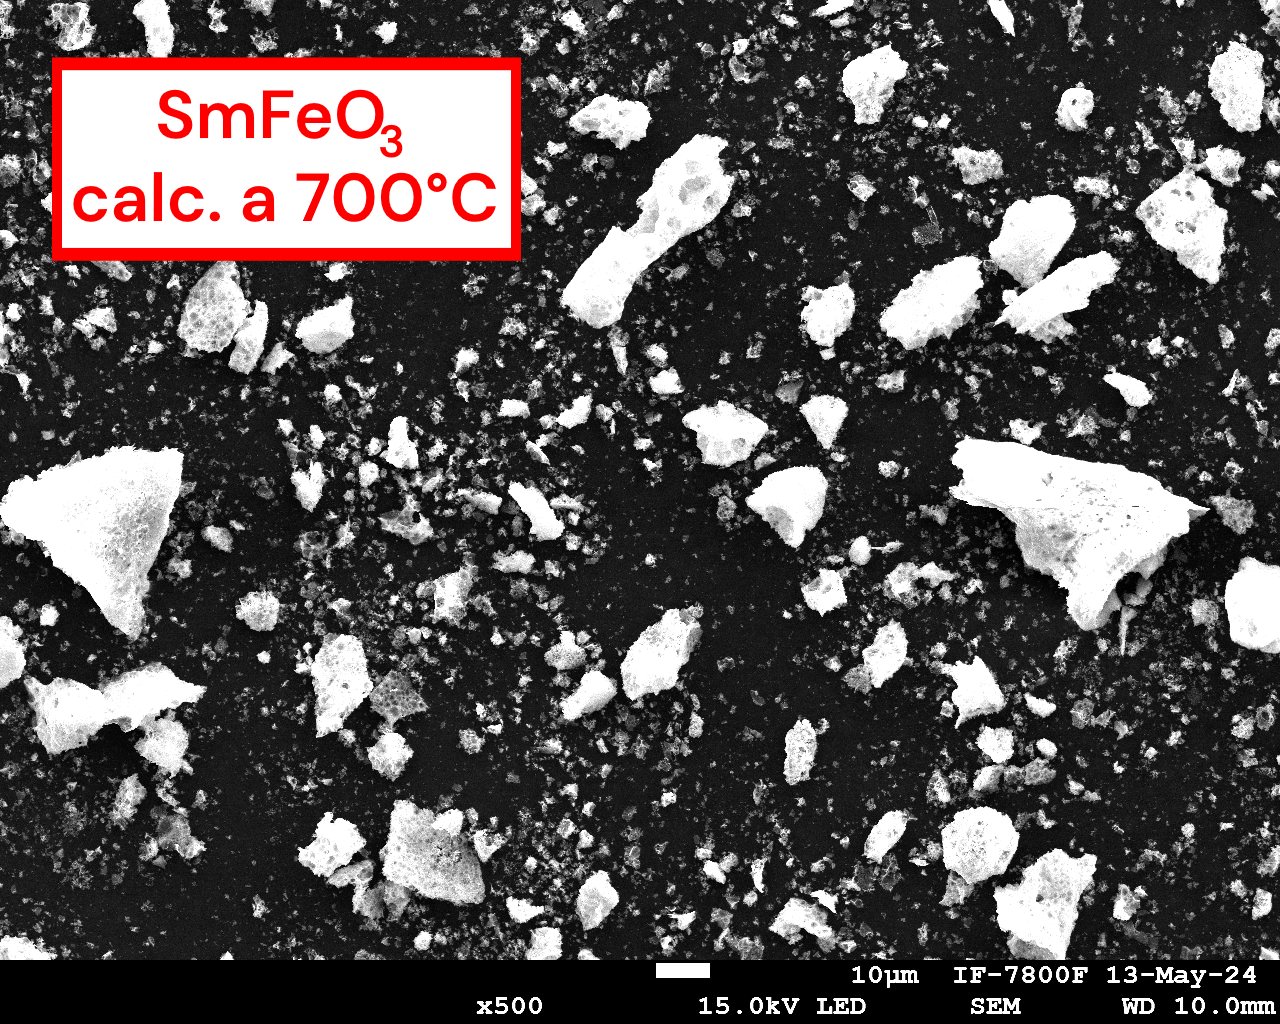
\includegraphics[width=0.45\textwidth]{fig/semsama700.png}
    \caption{Imágenes obtenidas a través de SEM para las muestras sin sonicar. Muestra de a) \neod{} calcinada a 600\gradoC{}, b) \sama{} calcinada a 700\gradoC{}. Amplificación $\times500$}
    \label{fig:resSEMsinsonicar}
\end{figure}
\begin{figure}[H]
    \centering
    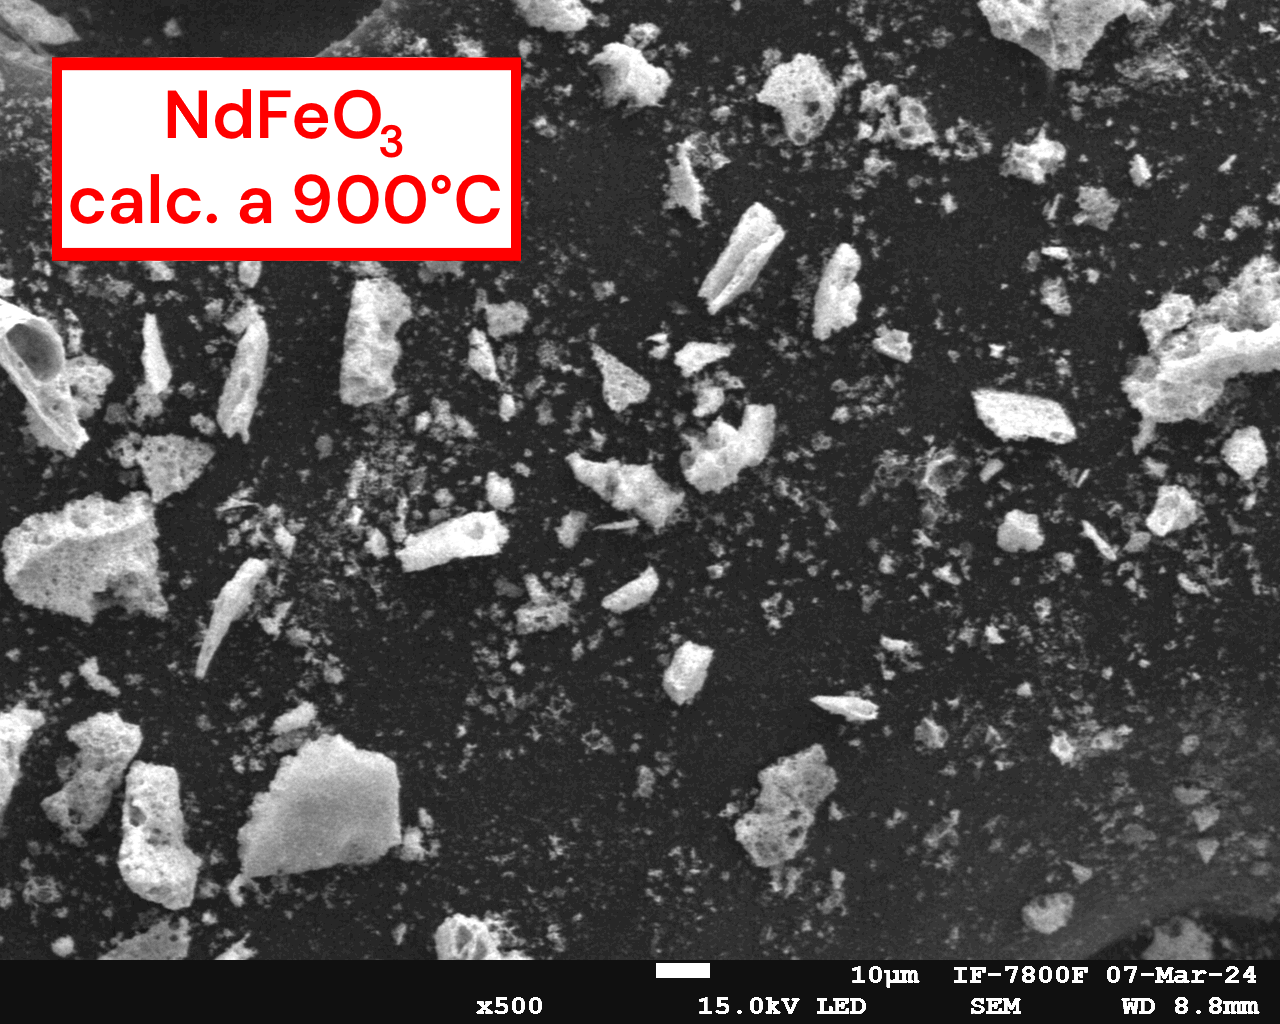
\includegraphics[width=0.45\textwidth]{fig/semneod900.png}
    \quad
    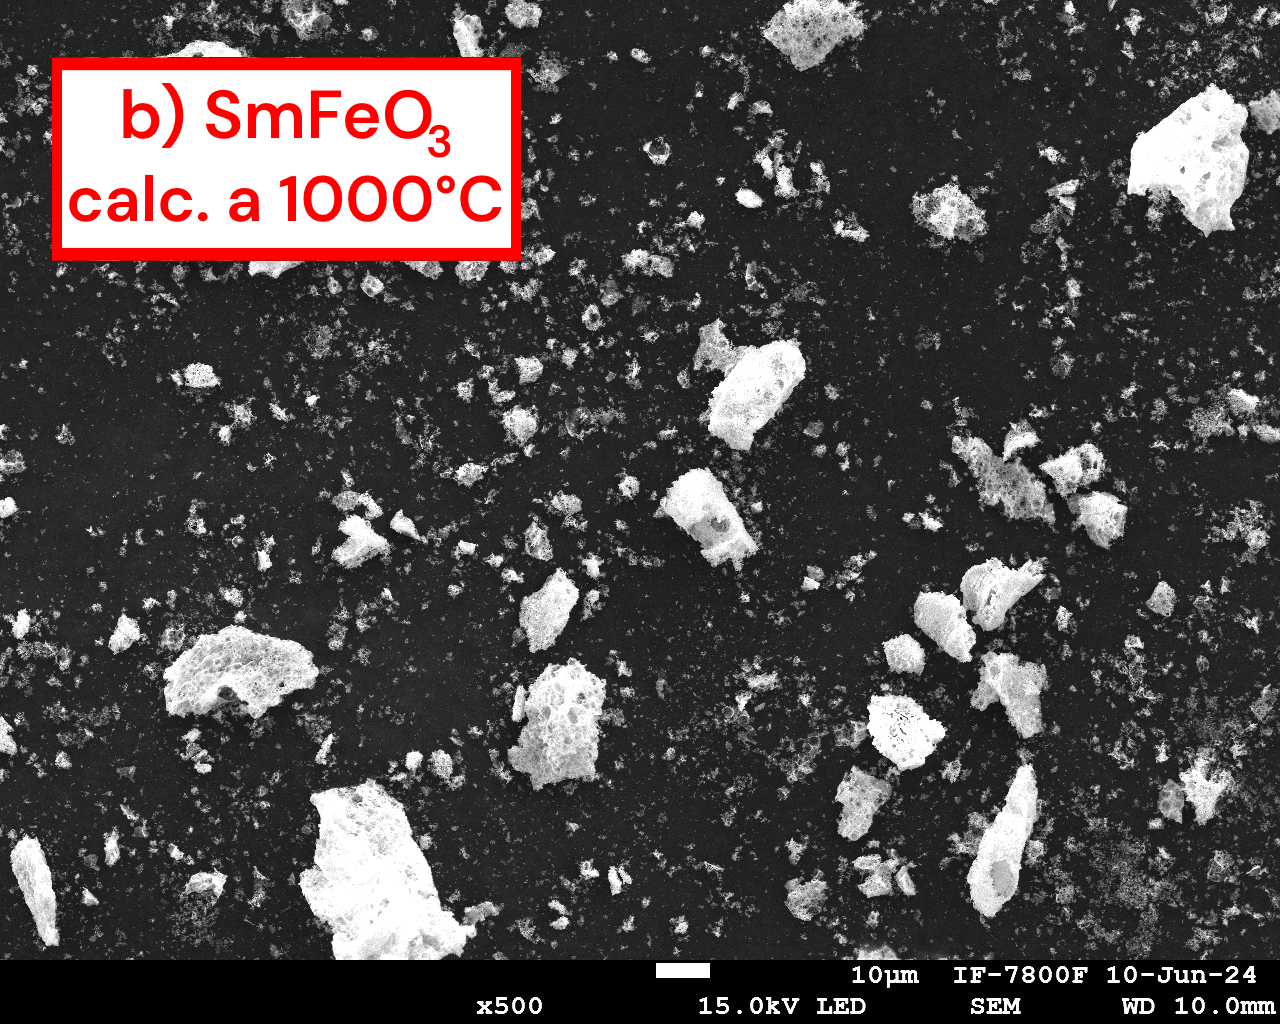
\includegraphics[width=0.45\textwidth]{fig/semsama1000.png}
    \caption{Imágenes obtenidas a través de SEM para las muestras sin sonicar. Muestra de a) \neod{} calcinada a 900\gradoC{}, b) \sama{} calcinada a 1000\gradoC{}. Amplificación $\times500$}
    \label{fig:resSEM900}
\end{figure}
\begin{figure}[H]
    \centering
    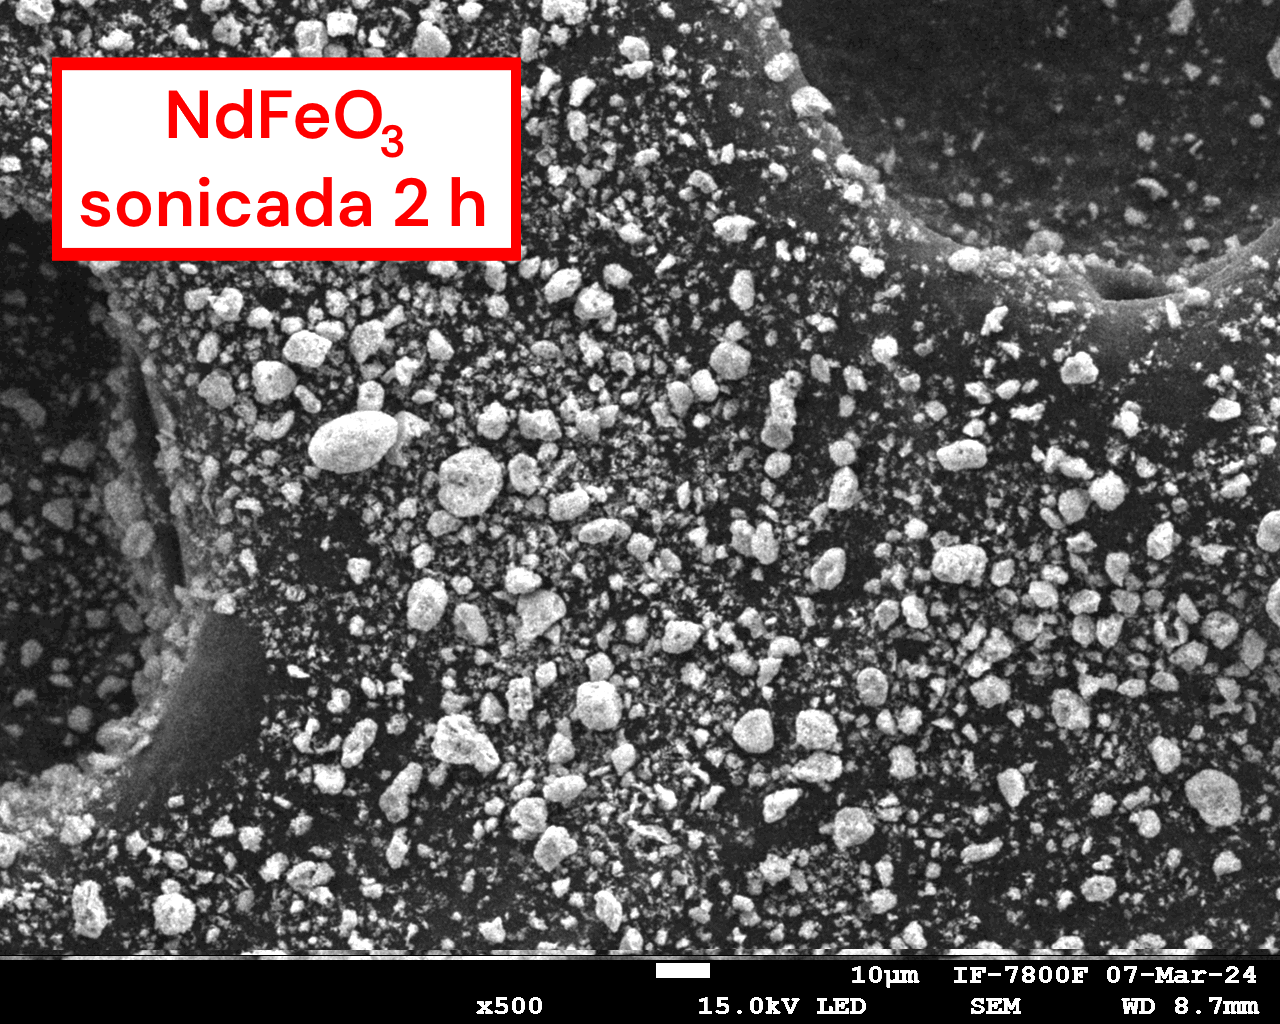
\includegraphics[width=0.45\textwidth]{fig/semneod2h.png}
    \quad
    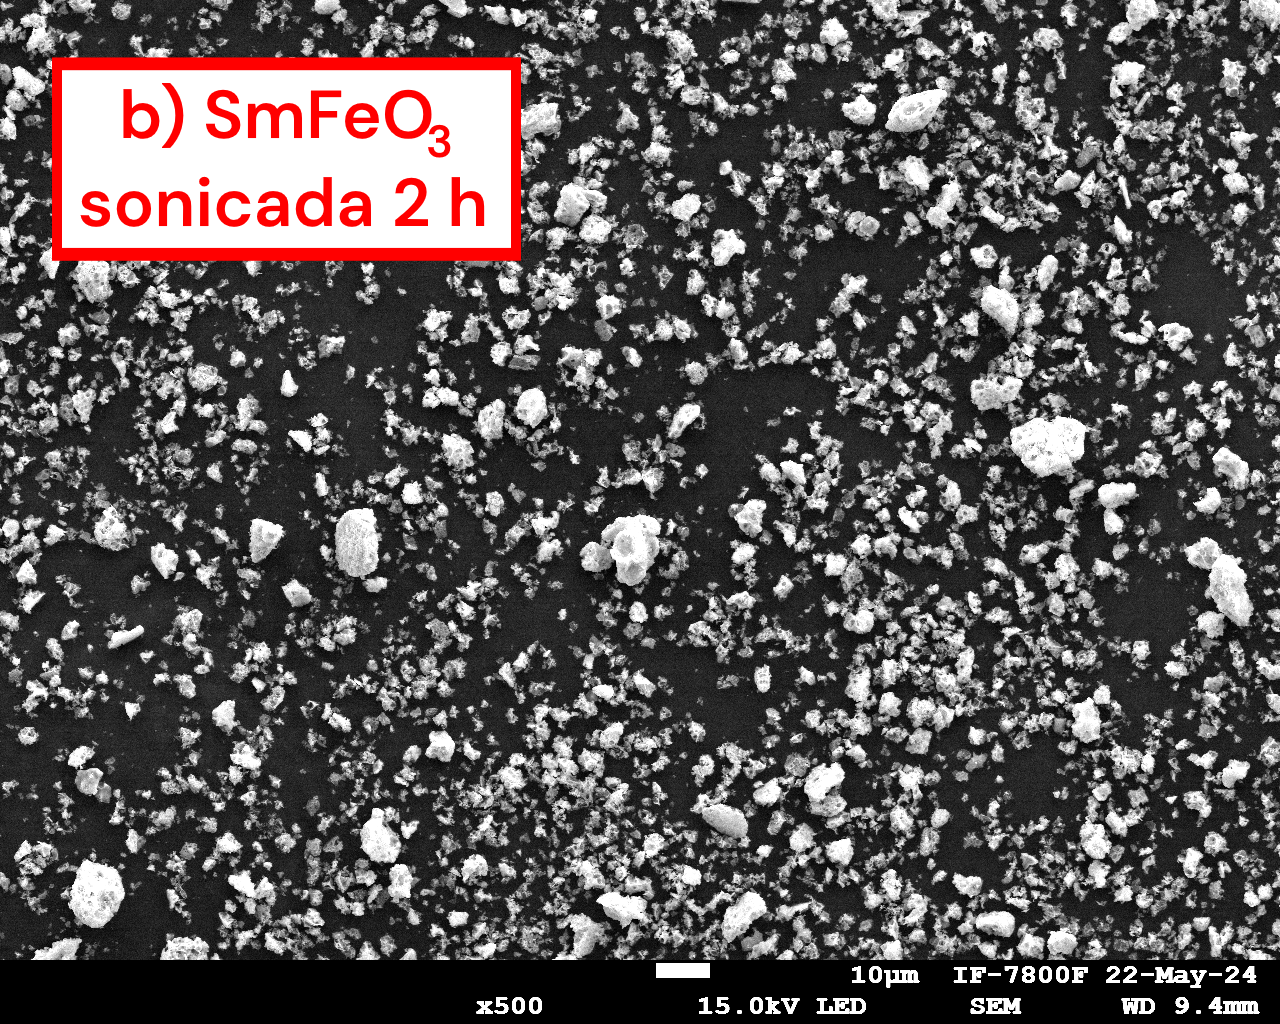
\includegraphics[width=0.45\textwidth]{fig/semsama2h.png}
    \caption{Imágenes obtenidas a través de SEM para las muestras sonicadas 2 horas. Muestra de a) \neod{} calcinada a 600\gradoC{}, b) \sama{} calcinada a 700\gradoC{}. Amplificación $\times500$}
    \label{fig:resSEMsonicada2}
\end{figure}
\begin{figure}[H]
    \centering
    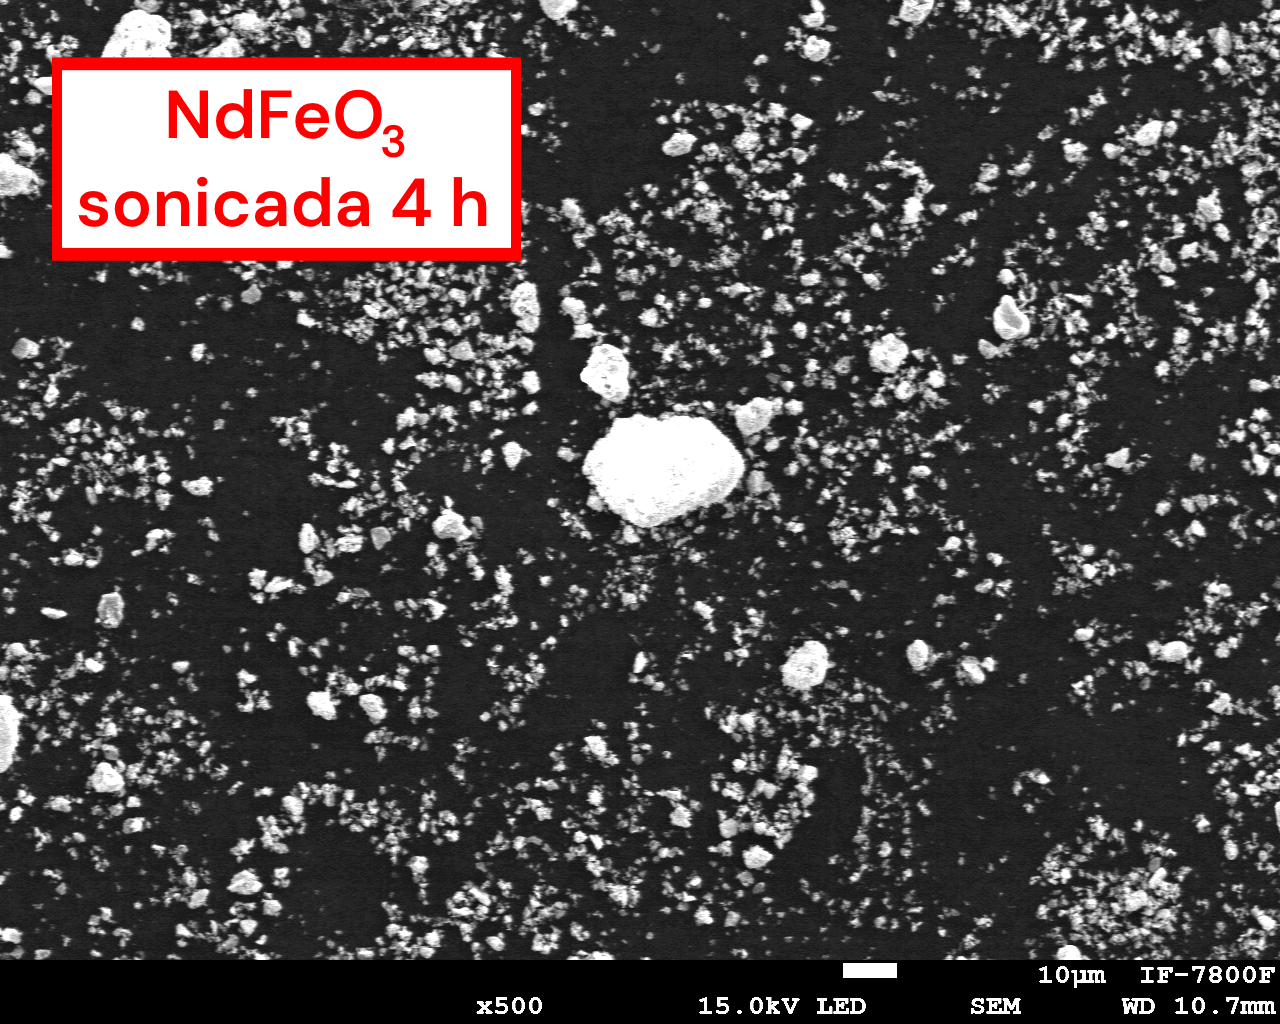
\includegraphics[width=0.45\textwidth]{fig/semneod4h.png}
    \quad
    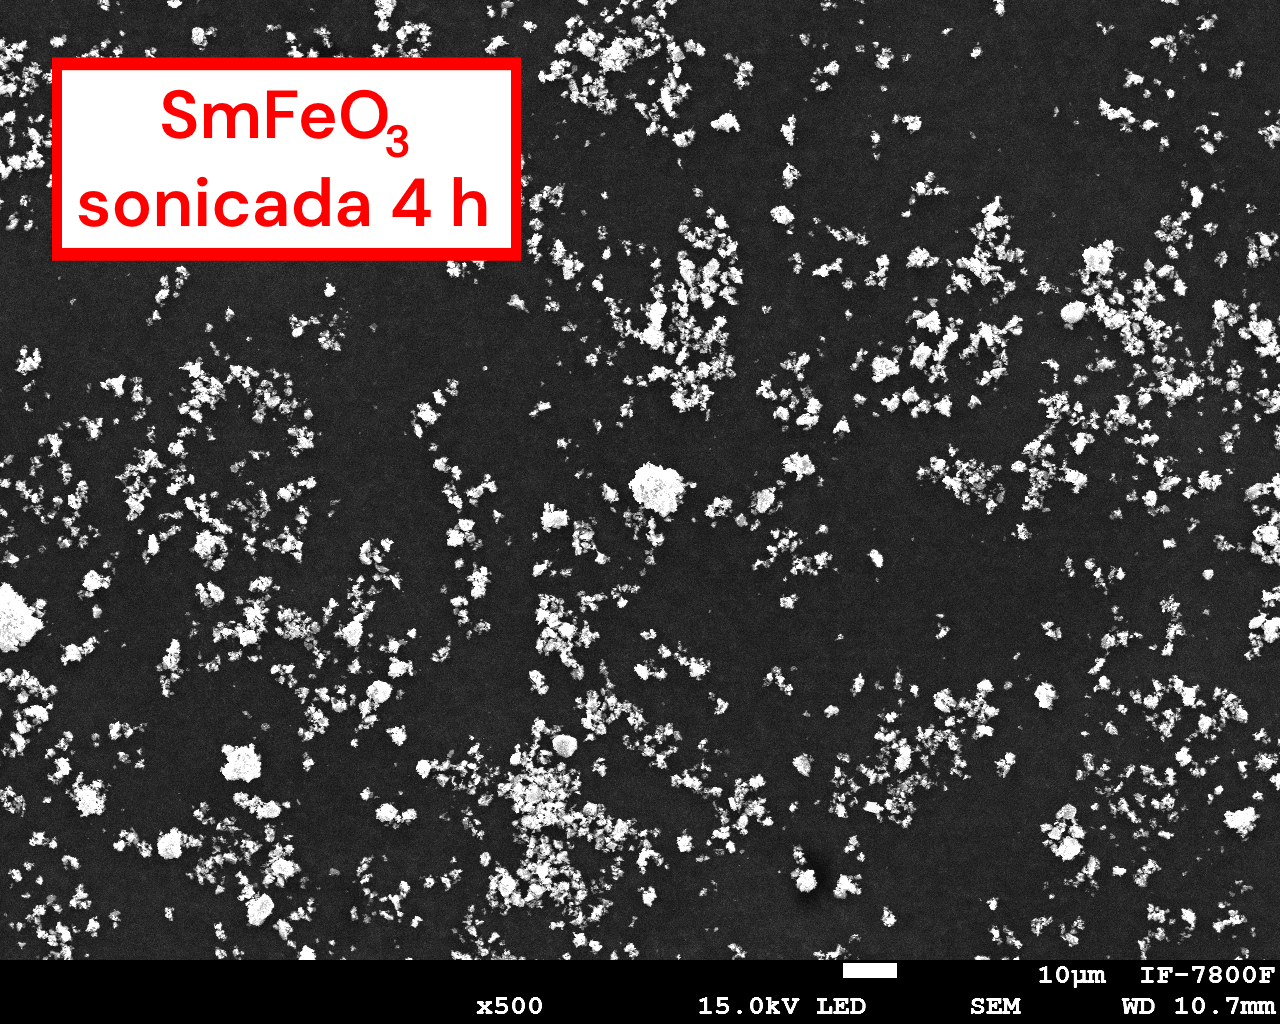
\includegraphics[width=0.45\textwidth]{fig/semsama4h.png}
    \caption{Imágenes obtenidas a través de SEM para las muestras sonicadas 4 horas. a) \neod{} calcinada a 600\gradoC{}, b) \sama{} calcinada a 700\gradoC{}. Amplificación $\times500$}
    \label{fig:resSEMsonicada4}
\end{figure}
Se observa que estas partículas presentan una estructura porosa independientemente de la temperatura, la cual se rompe después de ser sometida a un proceso de sonicación, siendo esto visible a simple vista al comparar las imágenes de las figuras \ref{fig:resSEMsinsonicar} y \ref{fig:resSEM900}, las cuales muestran a las ortoferritas de \neod{} calcinada a 600\gradoC{} y \sama{} calcinada a 700\gradoC{} respectivamente, con las que se encuentran en la figura \ref{fig:resSEMsonicada2}, en donde se muestran éstas mismas muestras después de ser sonicadas por 2 horas a 292W, además de las de la figura figura \ref{fig:resSEMsonicada4}, donde éstas muestras fueron sonicadas por 4 horas a la misma potencia. Tanto en la figura \ref{fig:resSEMsonicada2} como en \ref{fig:resSEMsonicada4}, se observa a simple vista que el tamaño de las partículas se vuelve mucho más homogéneo después del proceso de sonicación.

Como ya se describió en la sección \ref{sec:analisisestadistico}, los tamaños de partícula fueron obtenidos haciendo uso de \textit{ImageJ}.

Los métodos descritos en esa sección dieron como resultado los siguientes resultados:
\begin{table}[H]
    \centering
    \begin{tabular}{|c||c|c|c|}
        \hline
        Muestra & Temperatura de & Diámetro promedio & Porcentaje \\
        & calcinación & ($\mu$m) & $\leq1$ $\mu$m (\%) \\
        \hline
        \hline
        \multirow{6}{*}{\rotatebox[origin=c]{90}{\neod{}}} & 600\gradoC{} & 1.49$\pm$0.028 & 67.29$\pm$4.079 \\
        \cline{2-4}
        & 600\gradoC{}, sonicada 2 h & 1.00$\pm$0.035 & 80.87$\pm$0.799 \\
        \cline{2-4}
        & 600\gradoC{}, sonicada 4 h & 0.98$\pm$0.023 & 87.10$\pm$1.292 \\
        \cline{2-4}
        & 700\gradoC{} & 1.76$\pm$0.047 & 58.80$\pm$1.841 \\
        \cline{2-4}
        & 800\gradoC{} & 2.5$\pm$0.087 & 61.27$\pm$1.805 \\
        \cline{2-4}
        & 900\gradoC{} & 2.66$\pm$0.065 & 53.85$\pm$2.558 \\
        \hline
        \hline
        \multirow{6}{*}{\rotatebox[origin=c]{90}{\sama{}}} & 700\gradoC{} & 2.01$\pm$0.051 & 55.18$\pm$2.103 \\
        \cline{2-4}
        & 700\gradoC{}, sonicada 2 h & 1.81$\pm$0.037 & 88.13$\pm$1.080 \\
        \cline{2-4}
        & 700\gradoC{}, sonicada 4 h & 1.66$\pm$0.045 & 92.62$\pm$0.915 \\
        \cline{2-4}
        & 800\gradoC{} & 1.91$\pm$0.034 & 44.4$\pm$2.504 \\
        \cline{2-4}
        & 900\gradoC{} & 1.97$\pm$0.029 & 62.28$\pm$2.498 \\
        \cline{2-4}
        & 1000\gradoC{} & 2.02$\pm$0.055 & 44.46$\pm$2.640 \\
        \hline
\end{tabular}
    \caption{Tamaño promedio de partícula y porcentaje de partículas con diámetro $\leq$1 $\mu$m según la temperatura de calcinación para ambas ferritas.}
    \label{tabla:restamañoprom}
\end{table}
\begin{figure}[H]
    \centering
    \includegraphics[width=0.9\textwidth]{fig/restamañoprom.png}
    \caption{Tamaño promedio de partícula en función de la temperatura de calcinación. a) Muestras de \neod{}, b) muestras de \sama{}}
    \label{fig:restamañoprom}
\end{figure}
\begin{figure}[H]
    \centering
    \includegraphics[width=0.9\textwidth]{fig/resporcentaje.png}
    \caption{Porcentaje de partículas con diámetro $\leq$1 $\mu$m en función la temperatura de calcinación. a) Muestras de \neod{}, b) muestras de \sama{}}
    \label{fig:resporcentaje}
\end{figure}
Los datos que se muestran en la tabla \ref{tabla:restamañoprom} y graficados en la figura \ref{fig:restamañoprom} sugieren que el tamaño de partícula aumenta con la temperatura de calcinación, en particular para el \neod{}.

Por otro lado, la sonicación reduce considerablemente el tamaño promedio de partícula, además de aumentar el porcentaje de partículas con diámetro $\leq$1 $\mu$m como se ilustra en las figuras \ref{fig:restamañoprom} y \ref{fig:resporcentaje}.

Sin embargo, duplicar el tiempo de sonicación no cambia los resultados de manera significativa, por lo cual se piensa que este proceso sólo rompe las partículas más grandes, pero no es lo suficientemente potente para fragmentar las más pequeñas.
\subsection{Espectroscopía de dispersión de energía}
Como se explicó en la sección \ref{sec:electronsolido}, esta técnica reveló los elementos presentes en las muestras introducidas al microscopio electrónico de barrido, lo cual permite hallar posibles contaminantes, además de delimitar las posibles estructuras cristalinas a tomar en cuenta en el análisis de la difracción de rayos X de la sección \ref{sec:analisisDRX}.

En ninguna de las mediciones se encontraron contaminantes externos, a excepción de carbono, el cuál puede explicarse debido a que la cinta utilizada para la preparación de muestras está hecha de este material. En las figuras  \ref{fig:resEDSNeod} y \ref{fig:resEDSSama} se muestran las gráficas de cuentas obtenidas para cada elemento contra la energía de los electrones retrodispersados. En ambos casos se observa que los únicos elementos presentes son R=Nd, Sm, Fe, O y C. Esto se reporta cuantitativamente en las tablas \ref{tab:EDSNd} y \ref{tab:EDSSm}.
\begin{figure}[H]
    \centering
    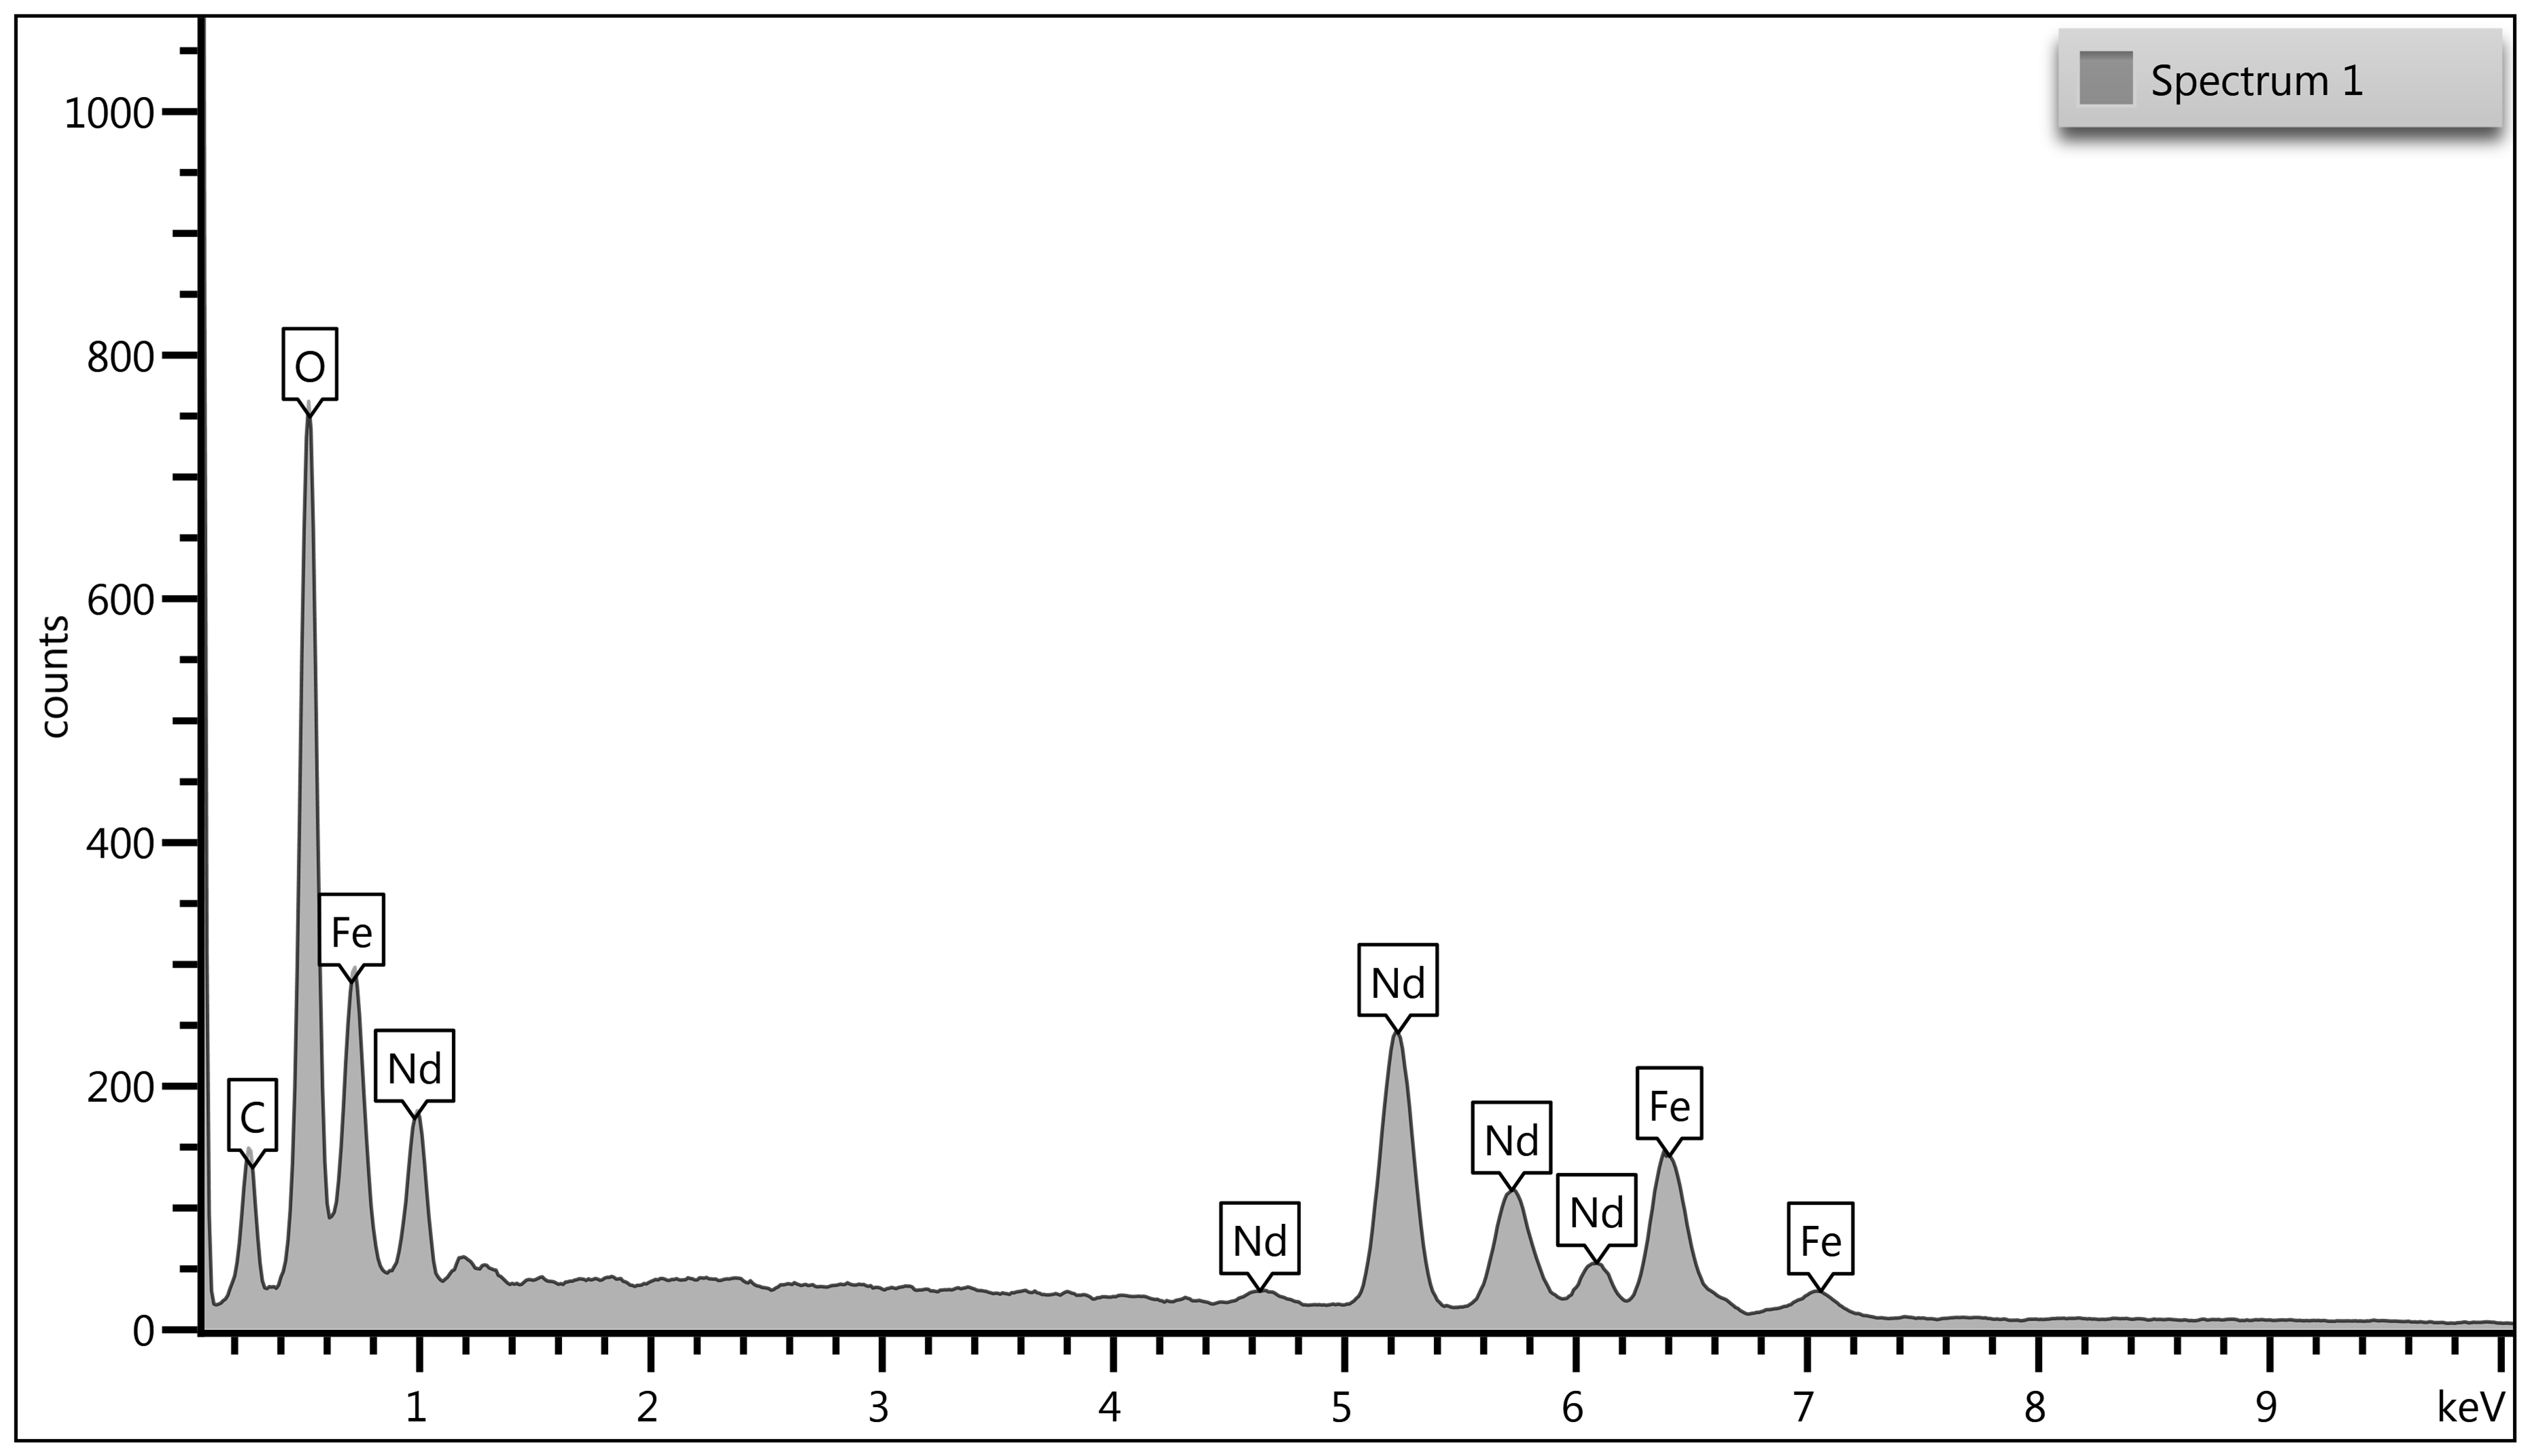
\includegraphics[width=0.7\textwidth]{fig/resEDSNeod.png}
    \caption{EDS de la muestra de \neod{} calcinada a 600\gradoC{} sin sonicar.}
    \label{fig:resEDSNeod}
\end{figure}
\begin{table}[H]
    \begin{tabular}{|c||c|c|c|c|c|c|c|}
        \hline
        Elem. &600\gradoC{} Son.&600\gradoC{} Son.&600\gradoC{}&700\gradoC{}&800\gradoC{}&900\gradoC{}&1000\gradoC{}\\
        &2h wt\%&4h wt\%&wt\%&wt\%&wt\%&wt\%&wt\%\\
        \hline\hline
        Fe & 20.33$\pm$0.78 &21.00$\pm$0.77& 19.94$\pm$0.68 & 22.23$\pm$1.01 & 20.31$\pm$0.67 & 21.0$\pm$1.04 & 18.37$\pm$2.06 \\
        Nd & 47.88$\pm$0.92 &58.44$\pm$0.87& 50.45$\pm$0.85 & 58.93$\pm$1.21 & 56.47$\pm$0.83 & 44.7$\pm$1.18 & 78.72$\pm$2.12 \\
        O & 31.79$\pm$0.70 &20.56$\pm$0.56& 21.71$\pm$0.54 & 11.04$\pm$0.57 & 15.06$\pm$0.45 & 20.4$\pm$0.57 & 2.92$\pm$0.60 \\
        C & 0 & 0 & 7.91$\pm$0.64 & 7.8$\pm$0.82 & 8.16$\pm$0.56 & 13.4$\pm$0.67 &0 \\ 
        \hline
        \end{tabular} 
            \caption{EDS de las muestras de \neod{}.}
            \label{tab:EDSNd}
        \end{table}
\begin{figure}[H]
    \centering
    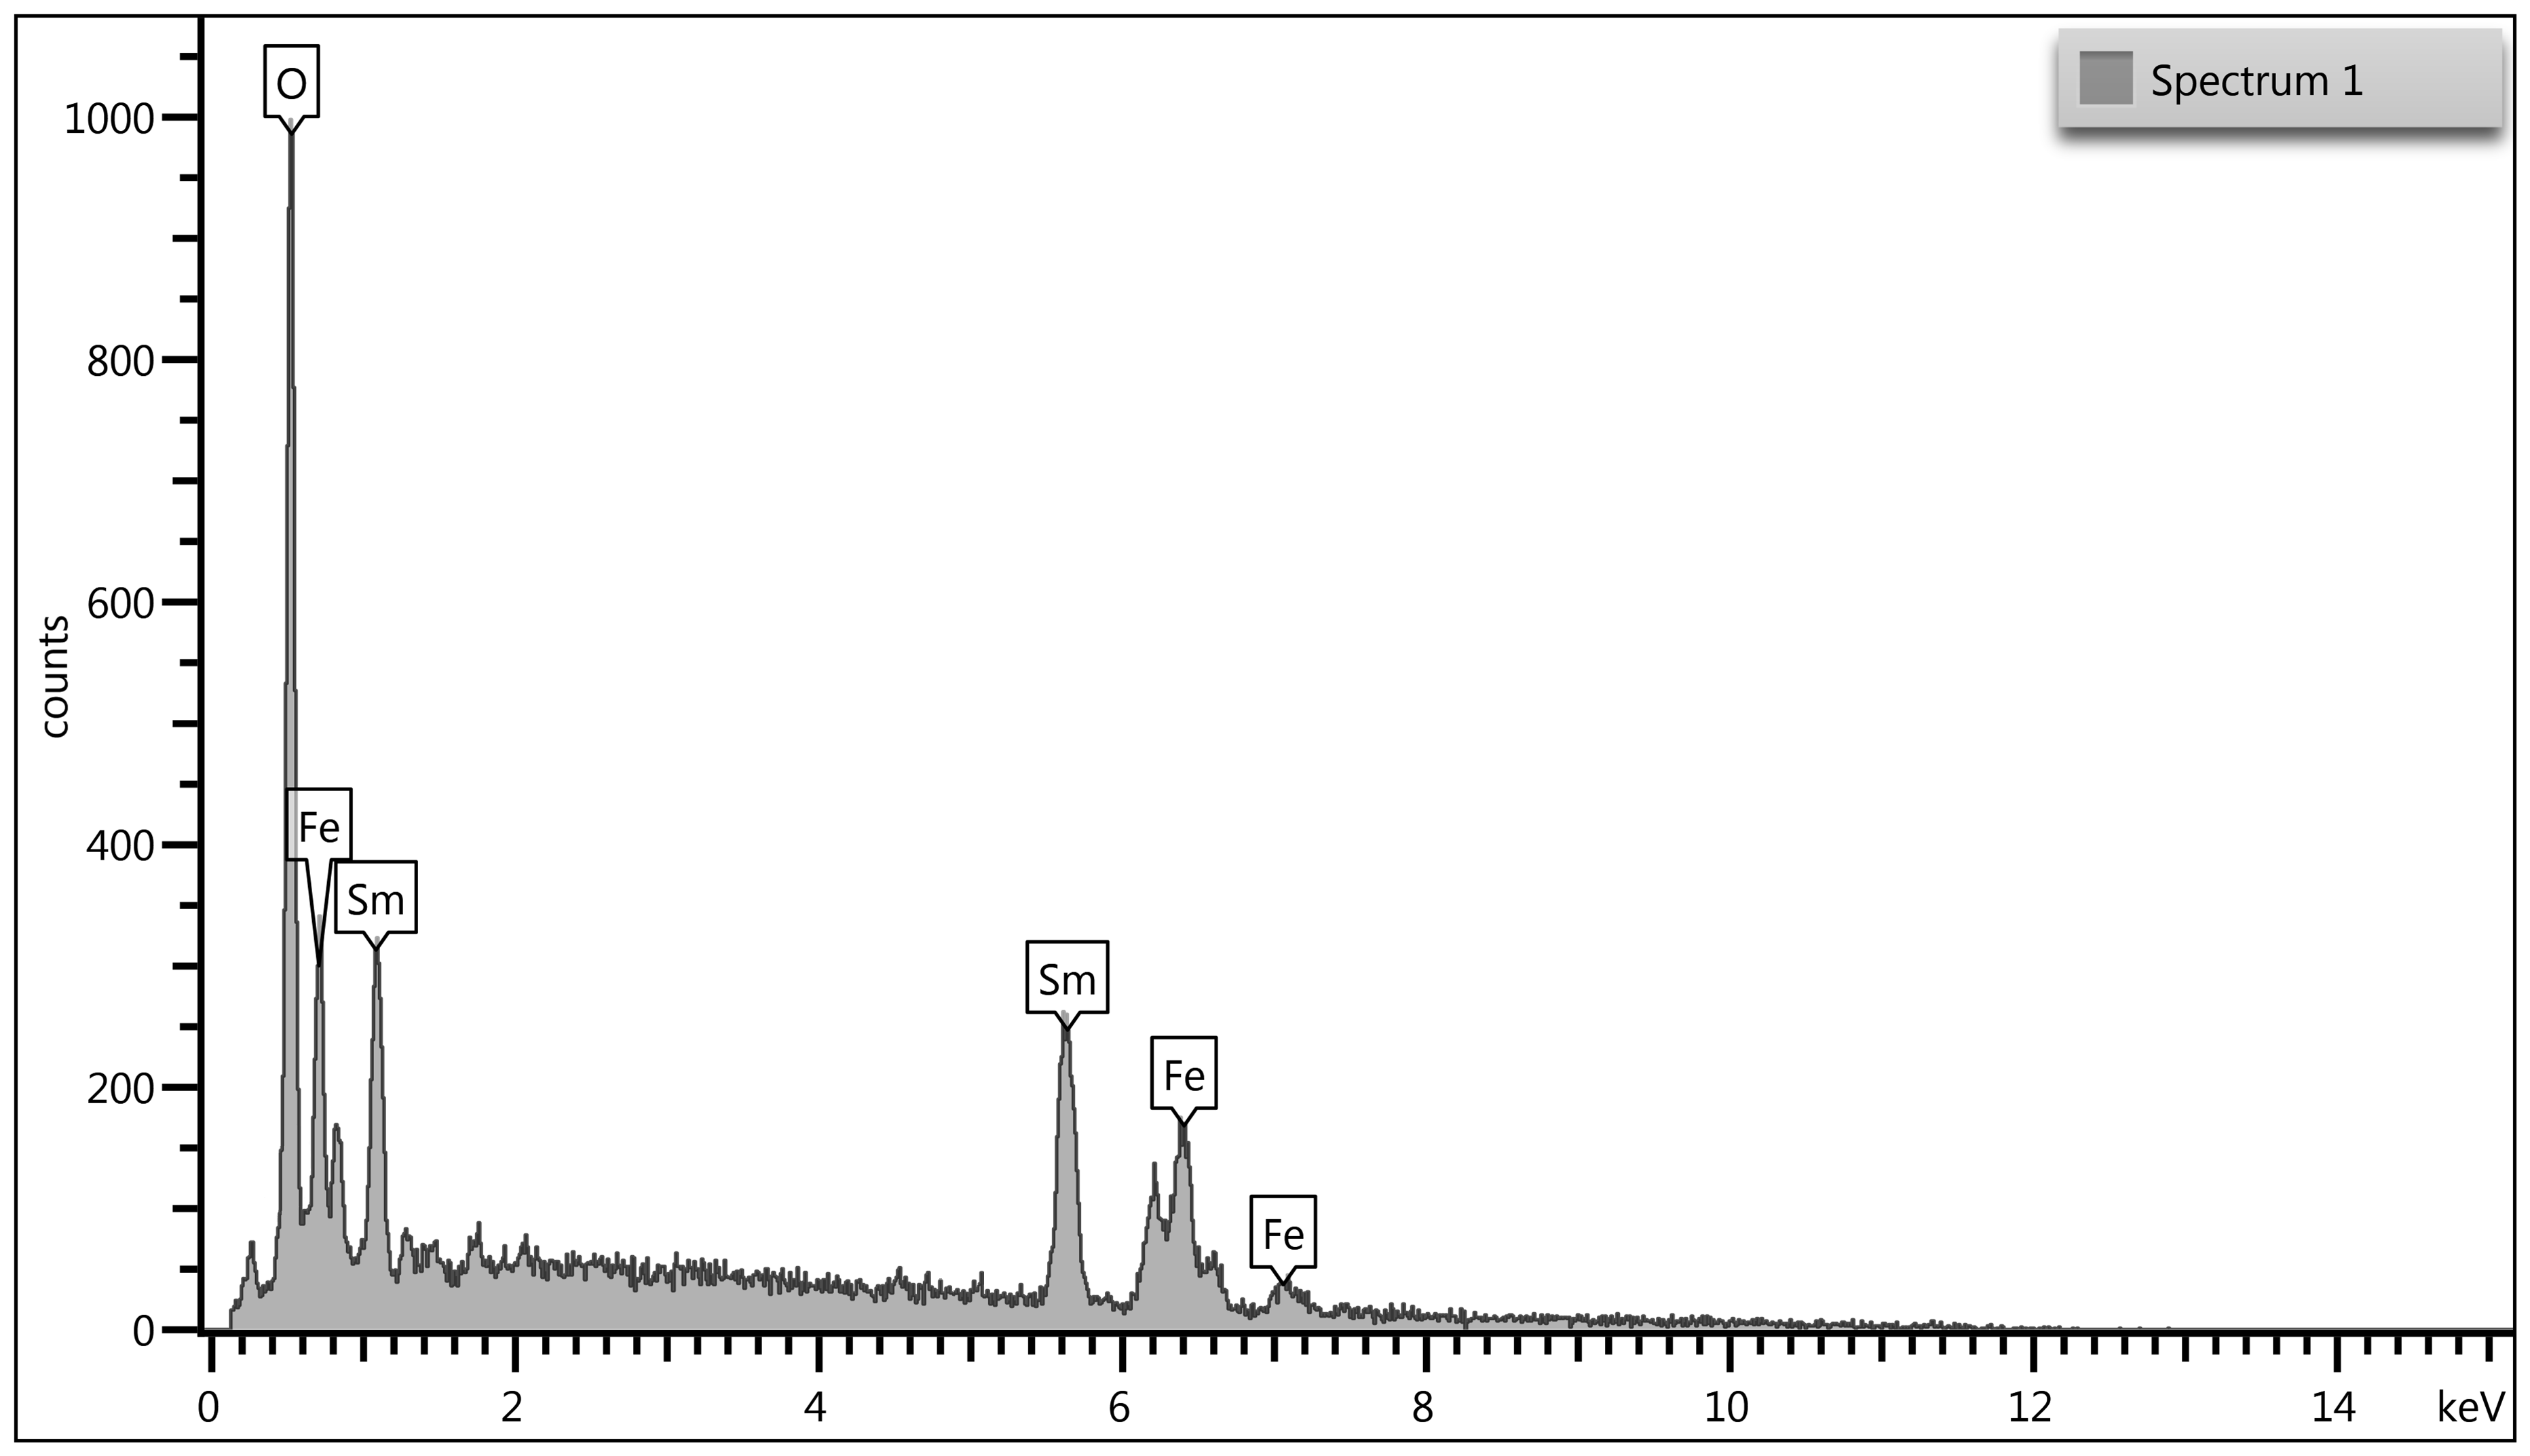
\includegraphics[width=0.7\textwidth]{fig/resEDSSama.png}
    \caption{EDS de la muestra de \sama{} calcinada a 700\gradoC{} sin sonicar.}
    \label{fig:resEDSSama}
\end{figure}
        \begin{table}[H]
            \centering
        \begin{tabular}{|c||c|c|c|c|c|c|}
        \hline
        Elem. &700\gradoC{} Son.&700\gradoC{} Son.&700\gradoC{}&800\gradoC{}&900\gradoC{}&1000\gradoC{}\\
        &2h wt\%&4h wt\%&wt\%&wt\%&wt\%&wt\%\\
        \hline\hline
        Fe &13.78$\pm$0.52&19.48$\pm$1.48& 7.51$\pm$0.42 & 22.31$\pm$0.93 & 22.51$\pm$3.03 & 17.44$\pm$0.83 \\
        Sm &38.42$\pm$0.74&48.22$\pm$1.95& 21.84$\pm$0.69 & 61.28$\pm$1.03 & 63.03$\pm$3.57 & 57.71$\pm$1.82 \\
        O &18.74$\pm$0.45&15.64$\pm$1.00& 15.95$\pm$0.47 & 16.41$\pm$0.58 & 14.46$\pm$1.78 & 20.81$\pm$0.78 \\
        C &29.16$\pm$0.62&16.66$\pm$1.53& 0 & 54.68$\pm$0.77 & 0 & 4.13$\pm$2.17 \\ 
        \hline
        \end{tabular} 
            \caption{EDS de las muestras de \sama{}.}
            \label{tab:EDSSm}
\end{table}
\subsection{Difracción de rayos X} \label{sec:analisisDRX}
A continuación se reportan los espectros obtenidos mediante la metodología descrita en \ref{sec:metodologiadrx} para cada temperatura de calcinación.
\begin{figure}[H]
    \centering
    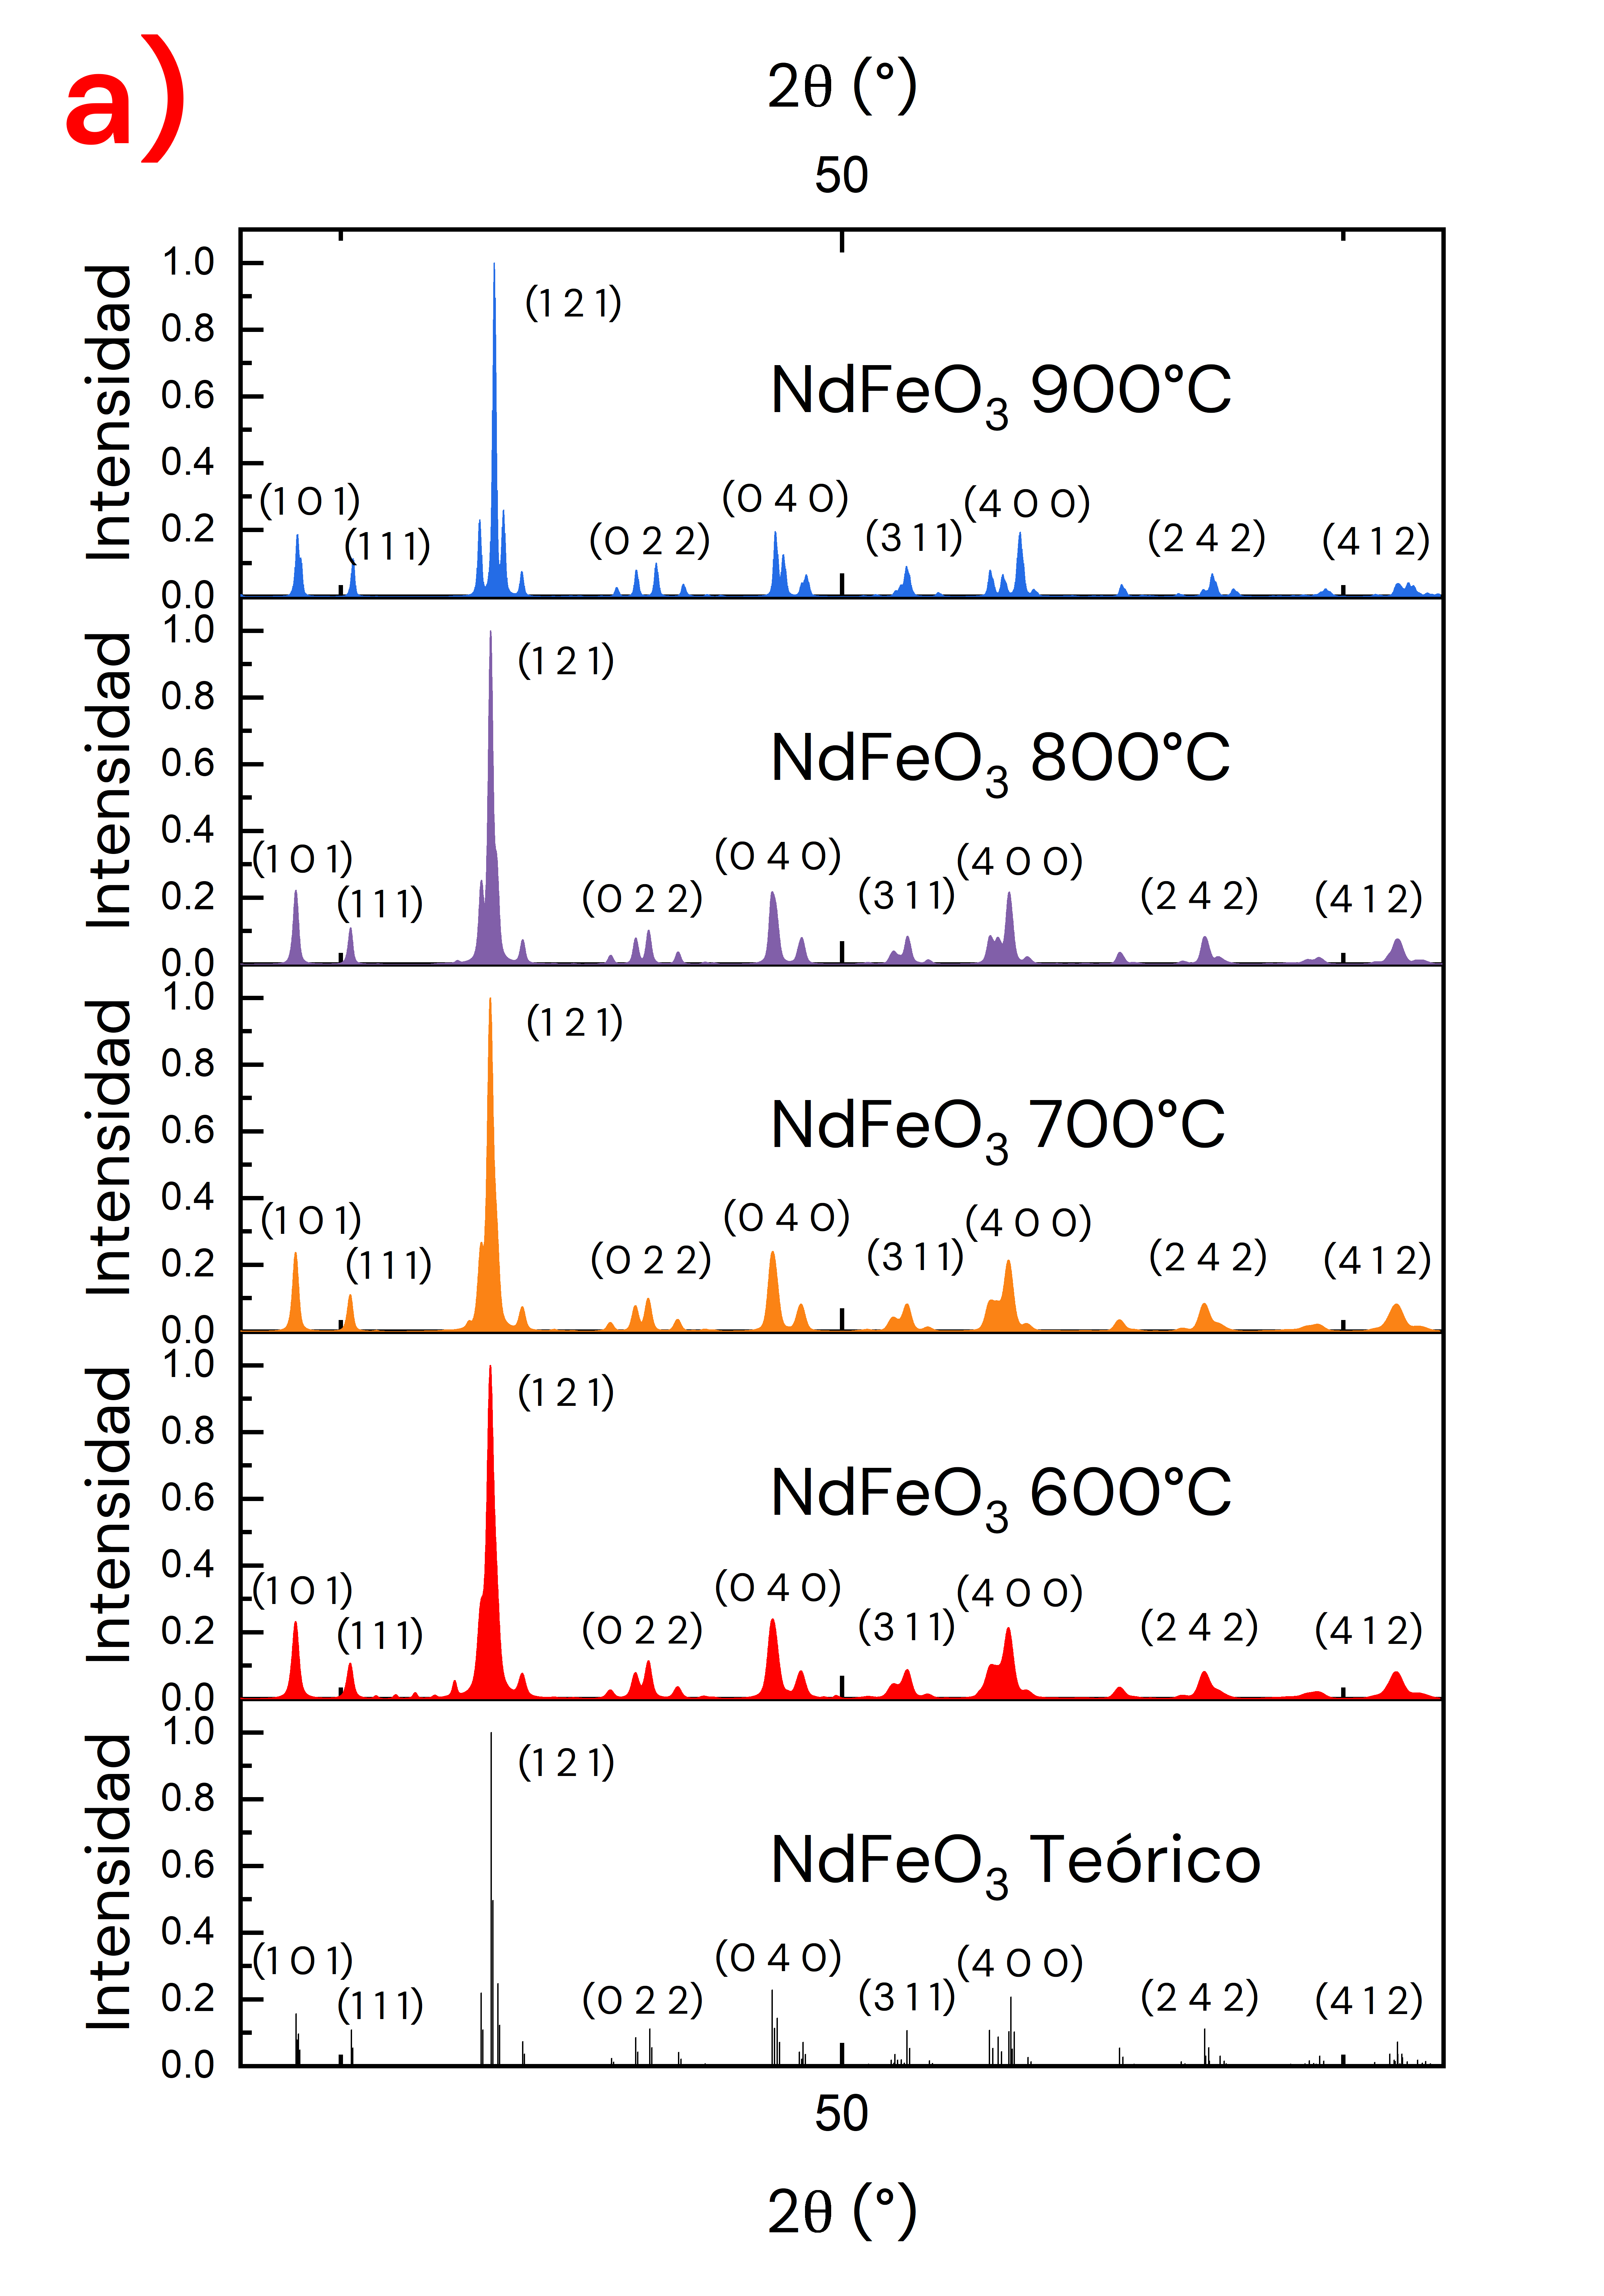
\includegraphics[width=0.45\textwidth]{fig/drxtempndfeo3.png}
    \quad
    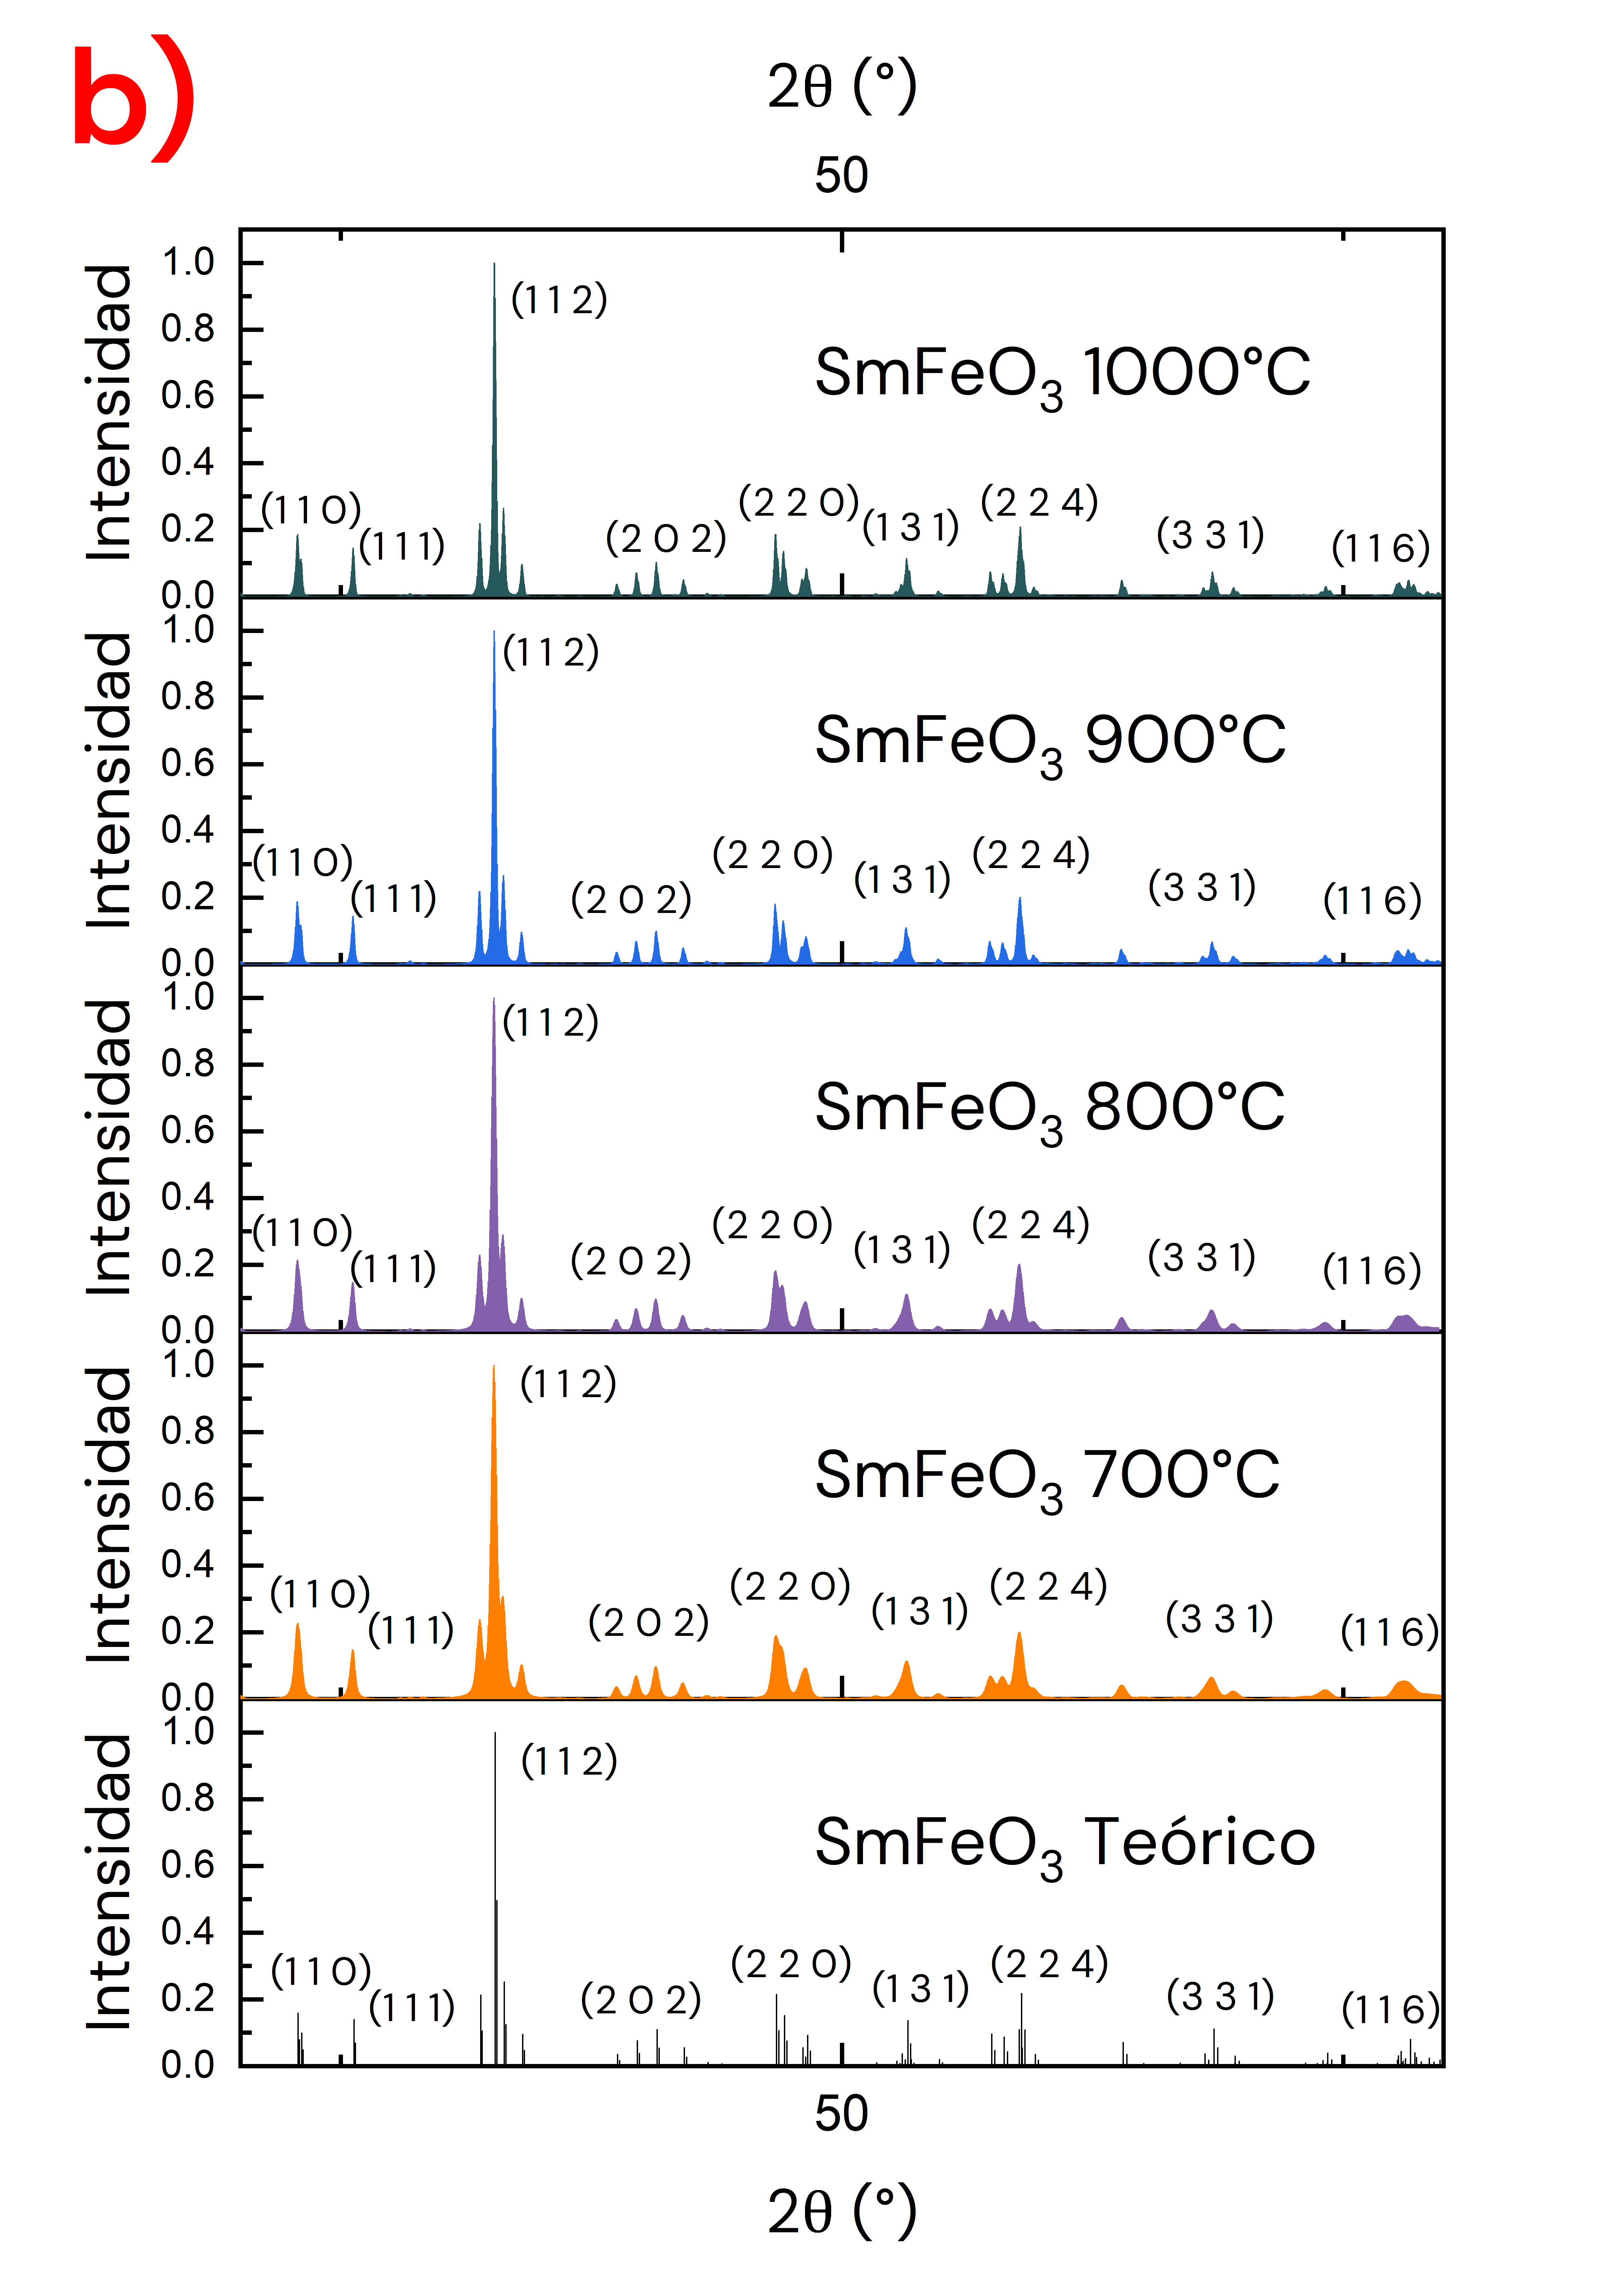
\includegraphics[width=0.45\textwidth]{fig/drxtempsmfeo3.png}
    \caption{Espectros obtenidos mediante DRX de las muestras calcinadas a distintas temperaturas. a) Muestras de \neod{}, b) Muestras de \sama{}. En cada gráfica se indican entre paréntesis los ángulos de difracción para diferentes planos obtenidos de \cite{ndfeo3} y \cite{smfeo3} respectivamente, así como la temperatura de calcinación de cada muestra.}
    \label{fig:drxtempcomp}
\end{figure}
Se puede observar que la posición de los picos obtenidos coinciden con los ángulos de difracción  de la estructura \textit{Pbnm} reportada en \cite{ndfeo3} para el \neod{} y en \cite{smfeo3} para el \sama{} respectivamente.

En la figure \ref{fig:drxtempcomp} se observa que el pico principal se hace más angosto y los picos alrededor de éste se vuelven visibles al aumentar la temperatura de calcinación entre 700 y 900\gradoC{}, especialmente para el \neod{}, esto sugiere que a medida que se aumenta la temperatura de calcinación los granos cristalinos van aumentando sus dimensiones, es decir, cuando la temperatura de calcinación están entre 600-800°C, el cristal ya ha adoptado una estructura $Pbnm$ (no hay señales de estructuras amorfas), sin embargo los granos cristalinos son relativamente pequeños, en cambio por encima de 800°C, los granos cristalinos tienen dimensiones mayores. Esto se discutirá a detalle en la sección \ref{sec:resrietlveld}.

A continuación se reportan los espectros obtenidos para las muestras sonicadas
\begin{figure}[H]
    \centering
    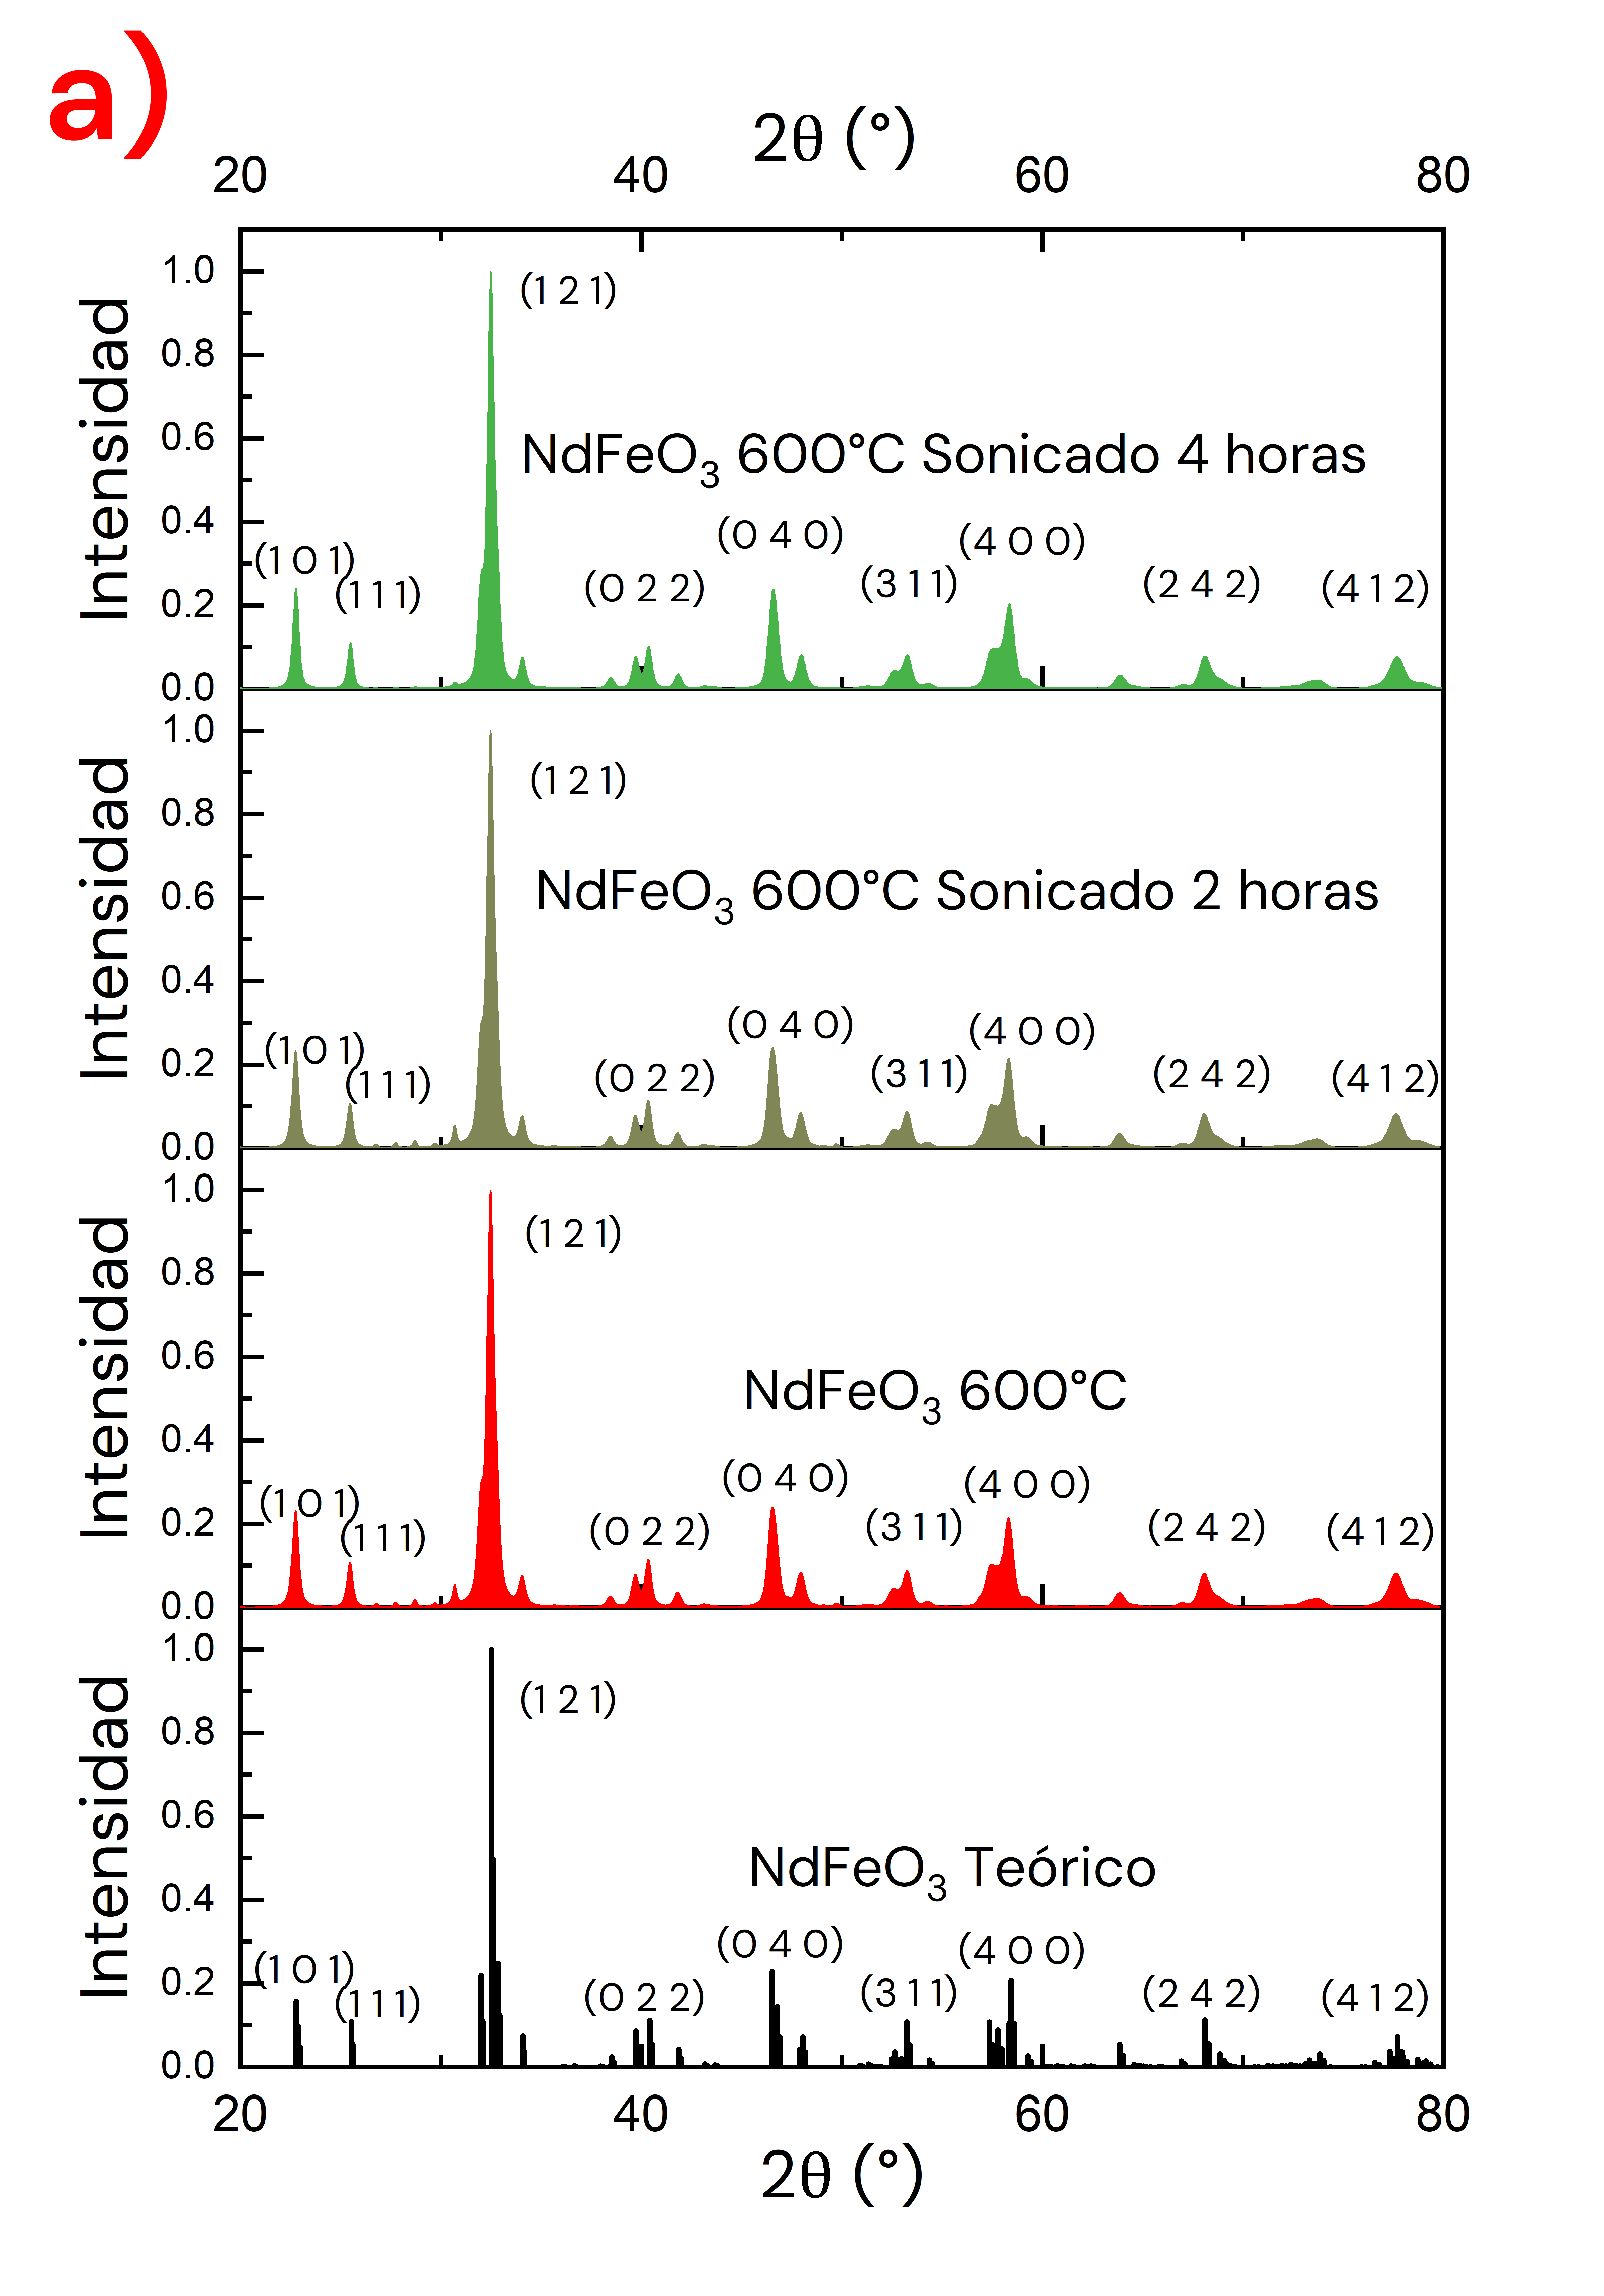
\includegraphics[width=0.45\textwidth]{fig/drxsonicndfeo3.png}
    \quad
    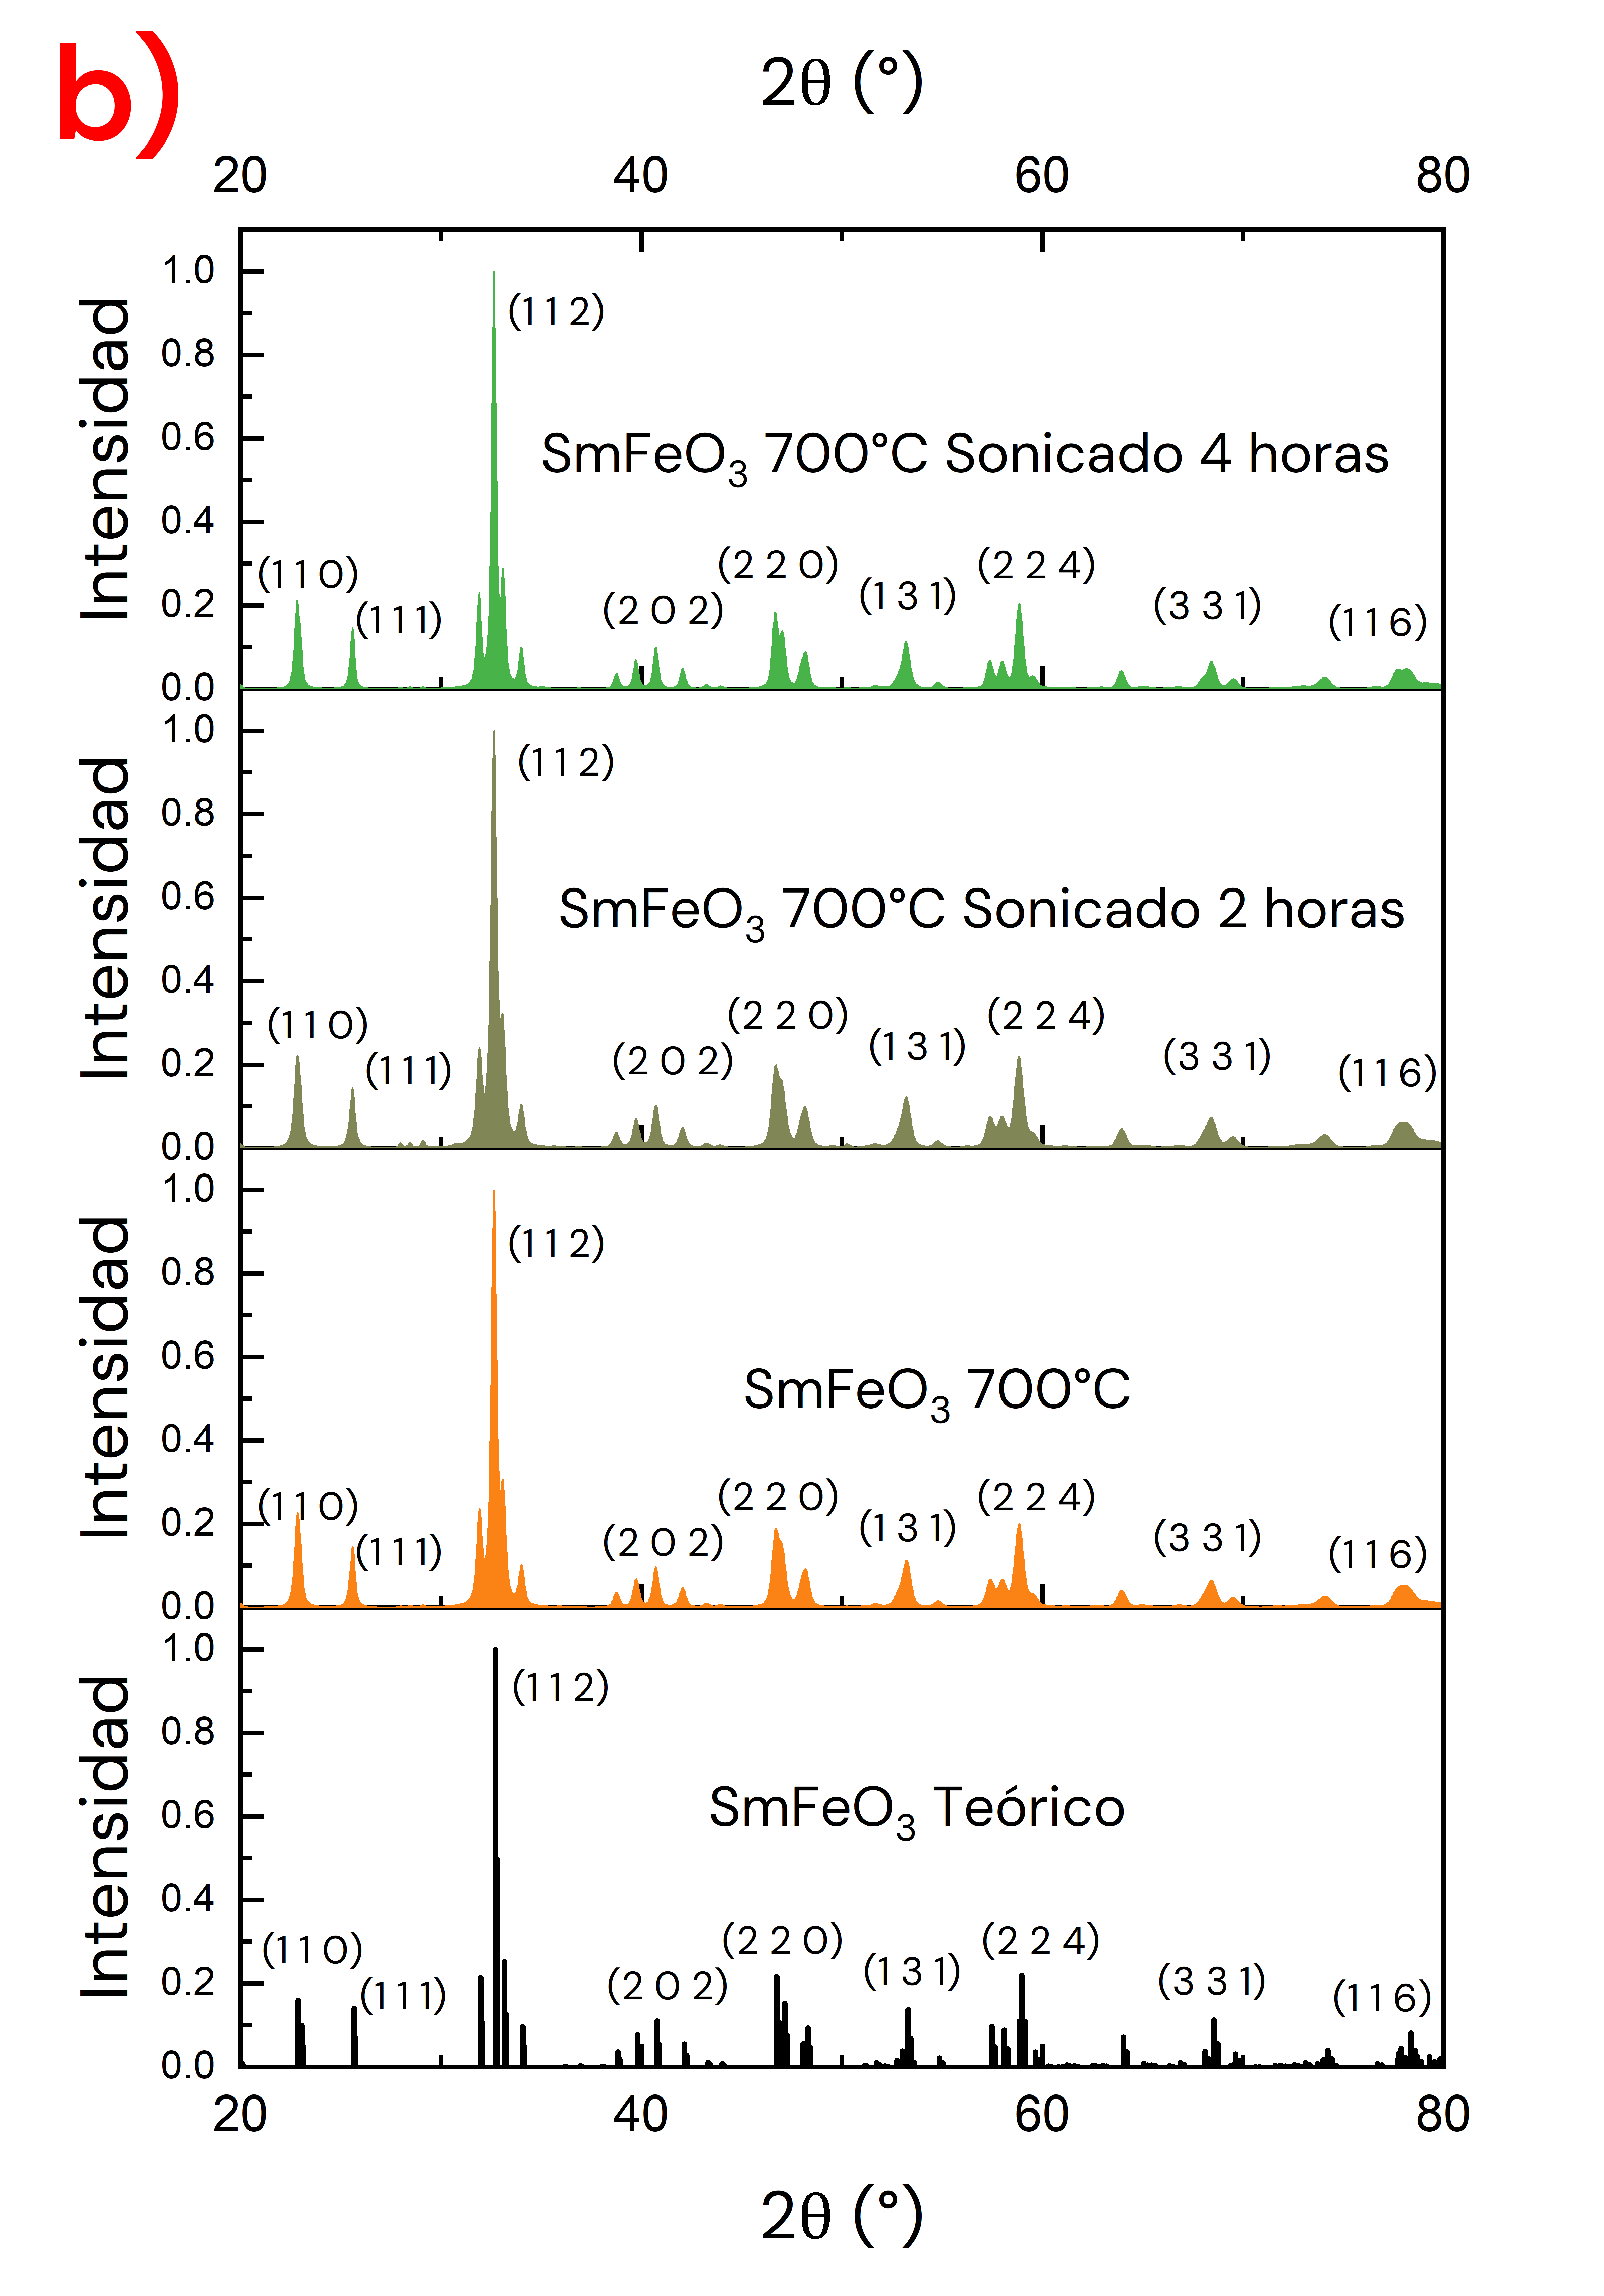
\includegraphics[width=0.45\textwidth]{fig/drxsonicsmfeo3.png}
    \caption{Espectros obtenidos mediante DRX de las muestras sonicadas. a) Muestras de \neod{}, b) Muestras de \sama{}. En cada gráfica se indican entre paréntesis los ángulos de difracción para diferentes planos obtenidos de \cite{ndfeo3} y \cite{smfeo3} respectivamente, así como el tiempo de sonicación de cada muestra.}
    \label{fig:drxsoniccomp}
\end{figure}
La figura \ref{fig:drxsoniccomp} muestra que el proceso de sonicación no modifica notoriamente el tamaño de grano cristalino, lo cual sugiere que el tamaño de grano que no necesariamente coincide con el tamaño de partícula ya que el análisis de tamaño de partícula a partir de las imágenes de SEM sí muestra un cambio en el diámetro promedio de partícula mediante el proceso de sonicación. Al variar el tiempo de sonicación, tampoco parece haber un cambio en la estructura cristalina.

\subsubsection{Refinamiento Rietveld} \label{sec:resrietlveld}
Mediante esta técnica se obtuvieron ajustes entre los difractogramas teóricos y los obtenidos experimentalmente, así como una estimación del porcentaje del peso que representa cada fase cristalina presente en la muestra (tablas \ref{tabla:refrietvneod} y \ref{tabla:refrietvsama}). Las figuras \ref{fig:rietveld600ndresultados} y \ref{fig:rietveld700smresultados}, son ejemplos típicos de estos ajustes entre el difractograma teórico (curva roja) y difractogramas medidos (puntos negros) para las composiciones \neod{} calcinada a 600\gradoC{} y \sama{} calcinada a 700\gradoC{} respectivamente:
\begin{figure}[H]
    \centering
    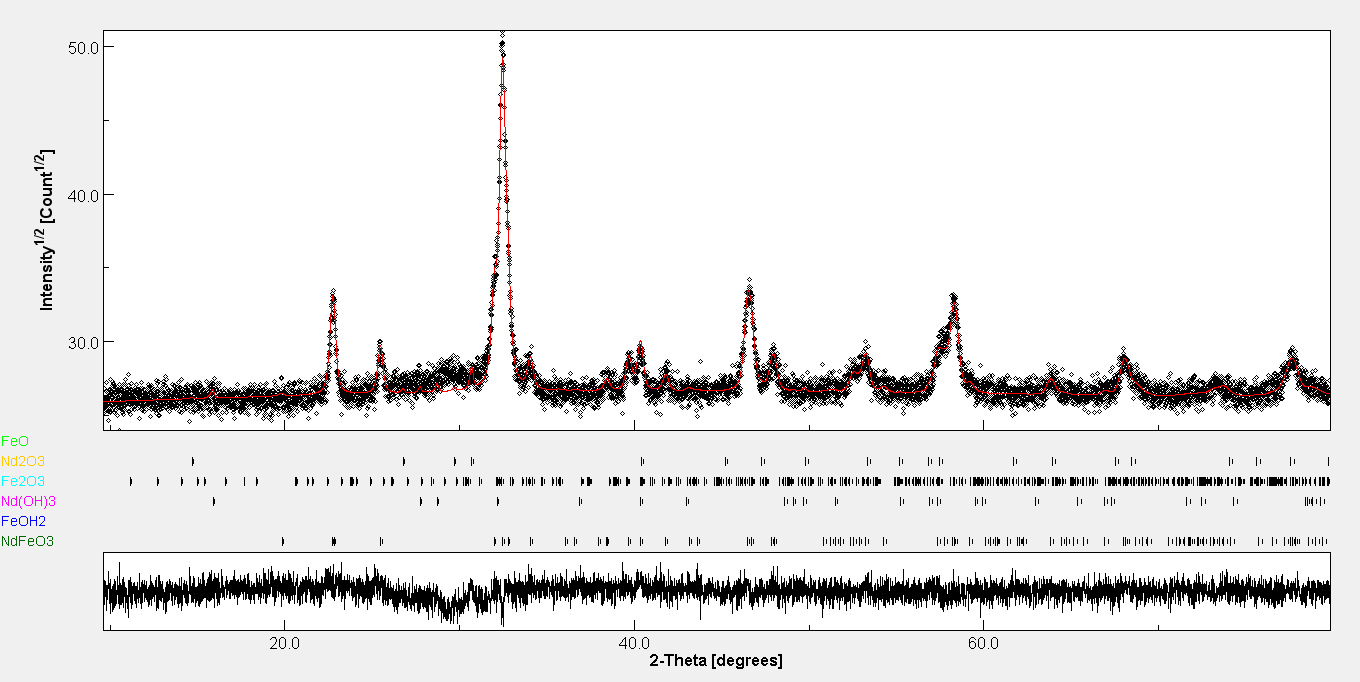
\includegraphics[width=0.8\textwidth]{fig/DRX600NdFeO3.png}
    \caption{Refinamiento Rietveld de la muestra de \neod{} calcinada a 600\gradoC{} sin sonicar. Los puntos negros son el espectro de difracción obtenido experimentalmente, la curva roja es el ajuste hecho por \textit{MAUD} (panel superior). Estructuras utilizadas: \neod{} \cite{ndfeo3}, \ce{Nd(OH)3} \cite{ndoh3}, \ce{Fe(OH)2} \cite{feoh2}, \ce{Nd2O3} \cite{nd2o3}, \ce{Fe2O3} \cite{fe2o3}, \ce{FeO} \cite{feo} (panel inferior).}
    \label{fig:rietveld600ndresultados}
\end{figure}
\begin{figure}[H]
    \centering
    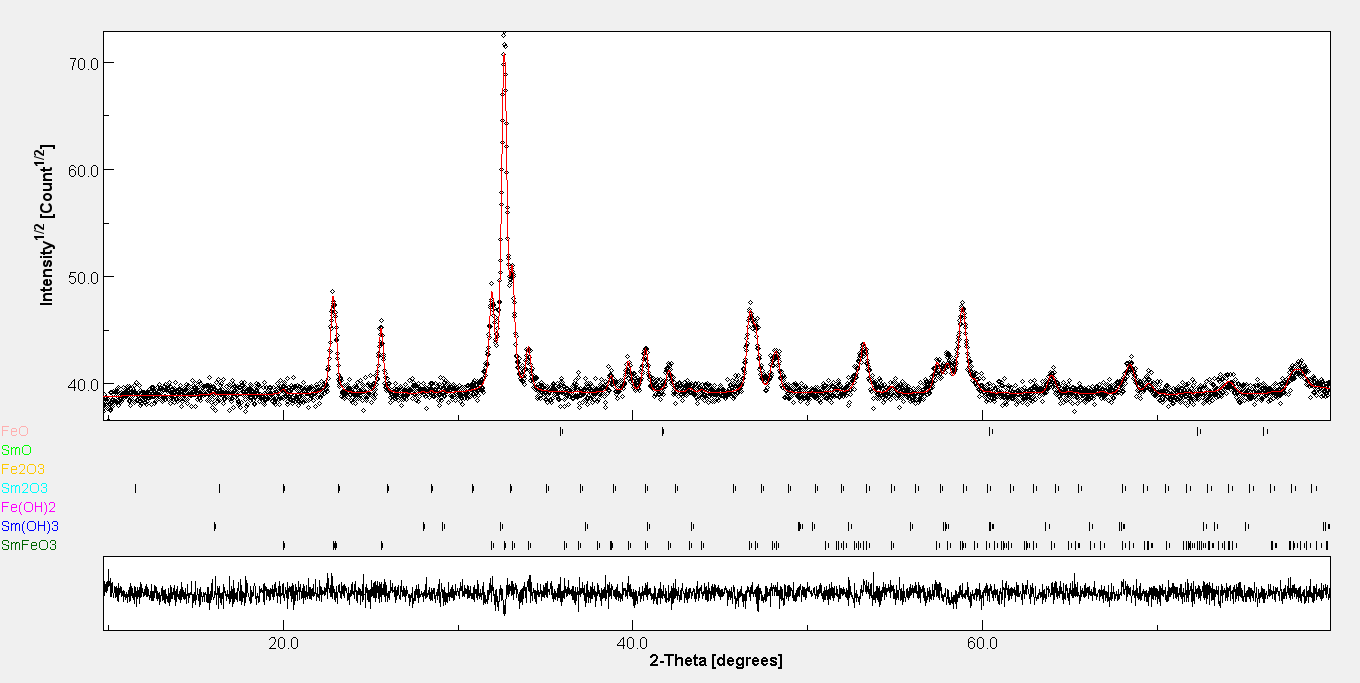
\includegraphics[width=0.8\textwidth]{fig/DRX700SmFeO3.png}
    \caption{Refinamiento Rietveld de la muestra de \sama{} calcinada a 00\gradoC{} sin sonicar. Los puntos negros son el espectro de difracción obtenido experimentalmente, la curva roja es el ajuste hecho por \textit{MAUD} (panel superior). Estructuras utilizadas: \sama{} \cite{smfeo3}, \ce{Sm(OH)3} \cite{smoh3}, \ce{Fe(OH)2} \cite{feoh2}, \ce{Sm2O3} \cite{sm2o3}, \ce{Fe2O3} \cite{fe2o3}, \ce{SmO} \cite{smo}, \ce{FeO} \cite{feo} (panel inferior).}
    \label{fig:rietveld700smresultados}
\end{figure}
El resto de refinamientos pueden encontrarse en el anexo \ref{sec:anexorietveld}.

Mediante estos refinamientos se encontró que las muestras contienen las siguientes composiciones en los porcentajes respectivos. Así mismo en la última columna se muestra el ajuste de bondad:
\begin{table}[H]
    \centering
    \begin{tabular}{|c||c|c|c|c|c|c|c|}
        \hline
        Muestra & \neod{} & \ce{Fe(OH)2} & \ce{Nd(OH)3} & \ce{Nd2O3} & \ce{Fe2O3} & \ce{FeO} & $\chi^2$ \\
        \hline
        \hline
        600\gradoC{} S 4 h & 98.81$\pm$0.0 & 0.61$\pm$0.782 & 0.26$\pm$0.170 & 0.30$\pm$0.111 & 0$\pm$0 & 0$\pm$0 & 1.08 \\
        \hline
        600\gradoC{} S 2 h & 95.73$\pm$0.0 & 0$\pm$0 & 1.38$\pm$0.231 & 2.62$\pm$0.188 & 0.24$\pm$0.649 & 0.00$\pm$0.309 & 1.21 \\
        \hline
        600\gradoC{} & 96.97$\pm$0.0 & 0$\pm$0 & 1.16$\pm$0.163 & 1.49$\pm$0.1312 & 0.37$\pm$0.457 & 0$\pm$0 & 1.12 \\
        \hline
        700\gradoC{} & 98.67$\pm$0.0 & 0$\pm$0 & 0$\pm$0 & 0.57$\pm$0.096 & 0.74$\pm$0.331 & 0$\pm$0 & 1.07 \\
        \hline
        800\gradoC{} & 98.67$\pm$0.0 & 0.40$\pm$0.632 & 0$\pm$0 & 0.33$\pm$0.088 & 0.58$\pm$0.319 & 0$\pm$0 & 1.05 \\
        \hline
        900\gradoC{} & 99.20$\pm$0.0 & 0$\pm$0 & 0$\pm$0 & 0.10$\pm$0.100 & 0.10$\pm$0.351 & 0.58$\pm$0.414 & 1.12 \\
        \hline
        \end{tabular} 
    \caption{Porcentaje del peso que representa cada una de las estructuras cristalinas presentes en cada muestra de \neod{}.}
    \label{tabla:refrietvneod}
\end{table}

\begin{table}[H]
    \centering
    \begin{tabular}{|c||c|c|c|c|c|c|c|}
        \hline
        Muestra & \sama{} & \ce{Sm(OH)3} & \ce{Fe(OH)2} & \ce{Sm2O3} & \ce{Fe2O3} & \ce{FeO} & $\chi^2$ \\ 
        \hline\hline
        700\gradoC{} S 4 h & 97.95$\pm$0.0 & 0.40$\pm$0.218 & 1.41$\pm$1.011 & 0.22$\pm$0.153 & 0$\pm$0 & 0$\pm$0 & 1.06 \\
        \hline
        700\gradoC{} S 2 h & 98.19$\pm$0.0 & 1.22$\pm$0.260 & 0$\pm$0 & 0.56$\pm$0.184 & 0$\pm$0 & 0$\pm$0 & 1.10 \\
        \hline
        700\gradoC{} & 99.17$\pm$0.0 & 0.35$\pm$0.176 & 0$\pm$0 & 0.19$\pm$0.150 & 0$\pm$0 & 0.27$\pm$0.358 & 1.07 \\
        \hline
        800\gradoC{} & 98.90$\pm$0.0 & 0.41$\pm$0.175 & 0$\pm$0 & 0.37$\pm$0.149 & 0$\pm$0 & 0.30$\pm$0.353 & 1.06 \\
        \hline
        900\gradoC{} & 98.65$\pm$0.0 & 0.41$\pm$0.178 & 0$\pm$0 & 0.69$\pm$0.151 & 0.23$\pm$0.484 & 0$\pm$0 & 1.08 \\
        \hline
        1000\gradoC{} & 97.56$\pm$0.0 & 0.70$\pm$0.177 & 0$\pm$0 & 0.64$\pm$0.149 & 0$\pm$0 & 1.08$\pm$0.348 & 1.09 \\
        \hline
        \end{tabular} 
    \caption{Porcentaje del peso que representa cada una de las estructuras cristalinas presentes en cada muestra de \sama{}.}
    \label{tabla:refrietvsama}
\end{table}
Se observa que el método de síntesis utilizado produce muestras de pureza alta, $\geq$95.73 para el \neod{} y $\geq$97.95 para el \sama{}. Por su parte, el valor de $\chi^2$ se encuentra en el rango establecido en \ref{sec:refinamiento} (1-1.3), teniendo como valor máximo 1.21, lo cual indica un buen ajuste en todos los refinamientos.

Por otro lado, los diámetros de cristal promedio se reportan en la tabla \ref{tabla:tamañoscristal}. Una gráfica de estos contra la temperatura de calcinación se encuentra en la figura \ref{fig:tamañoscristal} a) para el \neod{} y b) para el \sama{}.
\begin{table}[H]
    \centering
    \begin{tabular}{|c||c|c|}
        \hline
        Muestra & Diámetro promedio  & Incertidumbre (nm) \\
        & de cristal (nm) & \\
        \hline\hline
        \multicolumn{3}{|c|}{\neod{}} \\
        \hline
        600\gradoC{} sonicada 4 h & 578.48 & 12.570 \\
        \hline
        600\gradoC{} sonicada 2 h & 453.07 & 8.112 \\
        \hline
        600\gradoC{} & 472.90 & 9.688 \\
        \hline
        700\gradoC{} & 700.91 & 15.561 \\
        \hline
        800\gradoC{} & 836.31 & 9.327 \\
        \hline
        900\gradoC{} & 1670.95 & 43.745 \\
        \hline
        \multicolumn{3}{|c|}{\sama{}} \\
        \hline
        700\gradoC{} sonicada 4 h & 779.21 & 12.857 \\
        \hline
        700\gradoC{} sonicada 2 h & 542.23 & 12.739 \\
        \hline
        700\gradoC{} & 614.93 & 10.439 \\
        \hline
        800\gradoC{} & 829.59 & 22.802 \\
        \hline
        900\gradoC{} & 1647.29 & 35.357 \\
        \hline
        1000\gradoC{} & 2540.59 & 63.644 \\
        \hline
        \end{tabular} 
    \caption{Diámetro de cristal promedio reportados por Maud para las muestras de ambas ortoferritas.}
    \label{tabla:tamañoscristal}
\end{table}
\begin{figure}[H]
    \centering
    \includegraphics[width=0.4\textwidth]{fig/tamañocristalneod.png}
    \quad
    \includegraphics[width=0.4\textwidth]{fig/tamañocristalsama.png}
    \caption{Diámetro de cristal promedio contra temperatura de calcinación para las muestras de: a) \neod, b) \sama.}
    \label{fig:tamañoscristal}
\end{figure}
Se observa un crecimiento del diámetro de cristal con el aumento de temperatura, este se vuelve más pronunciado a partir de los 900\gradoC{}. La sonicación tuvo el mismo efecto en ambas muestras, reduciendo ligeramente el diámetro en las muestras sonicadas 2 horas, pero aumentando éste cuando se sonicaron por 4 horas, sin embargo, este efecto es menos pronunciado que el que ocurre producto del cambio de temperatura de calcinación.
\section{Caracterización óptica, magnética y eléctrica} \label{sec:analisisoptmagelec}
A continuación se presentan los resultados obtenidos para cada ortoferrita al realizar espectroscopía UV-Vis, magnetometría SQUID y mediciones de curvas de polarización.
\subsection{\texorpdfstring{\neod{}}{NdFeO3}}
\subsubsection{Espectroscopía UV-Vis}
Mediante la metodología descrita en la sección \ref{sec:uvvismetod} se obtuvieron las siguientes gráficas de absorbancia contra longitud de onda para las muestras de \neod{} (figura \ref{fig:absorbresneod}):
\begin{figure}[H]
    \centering
    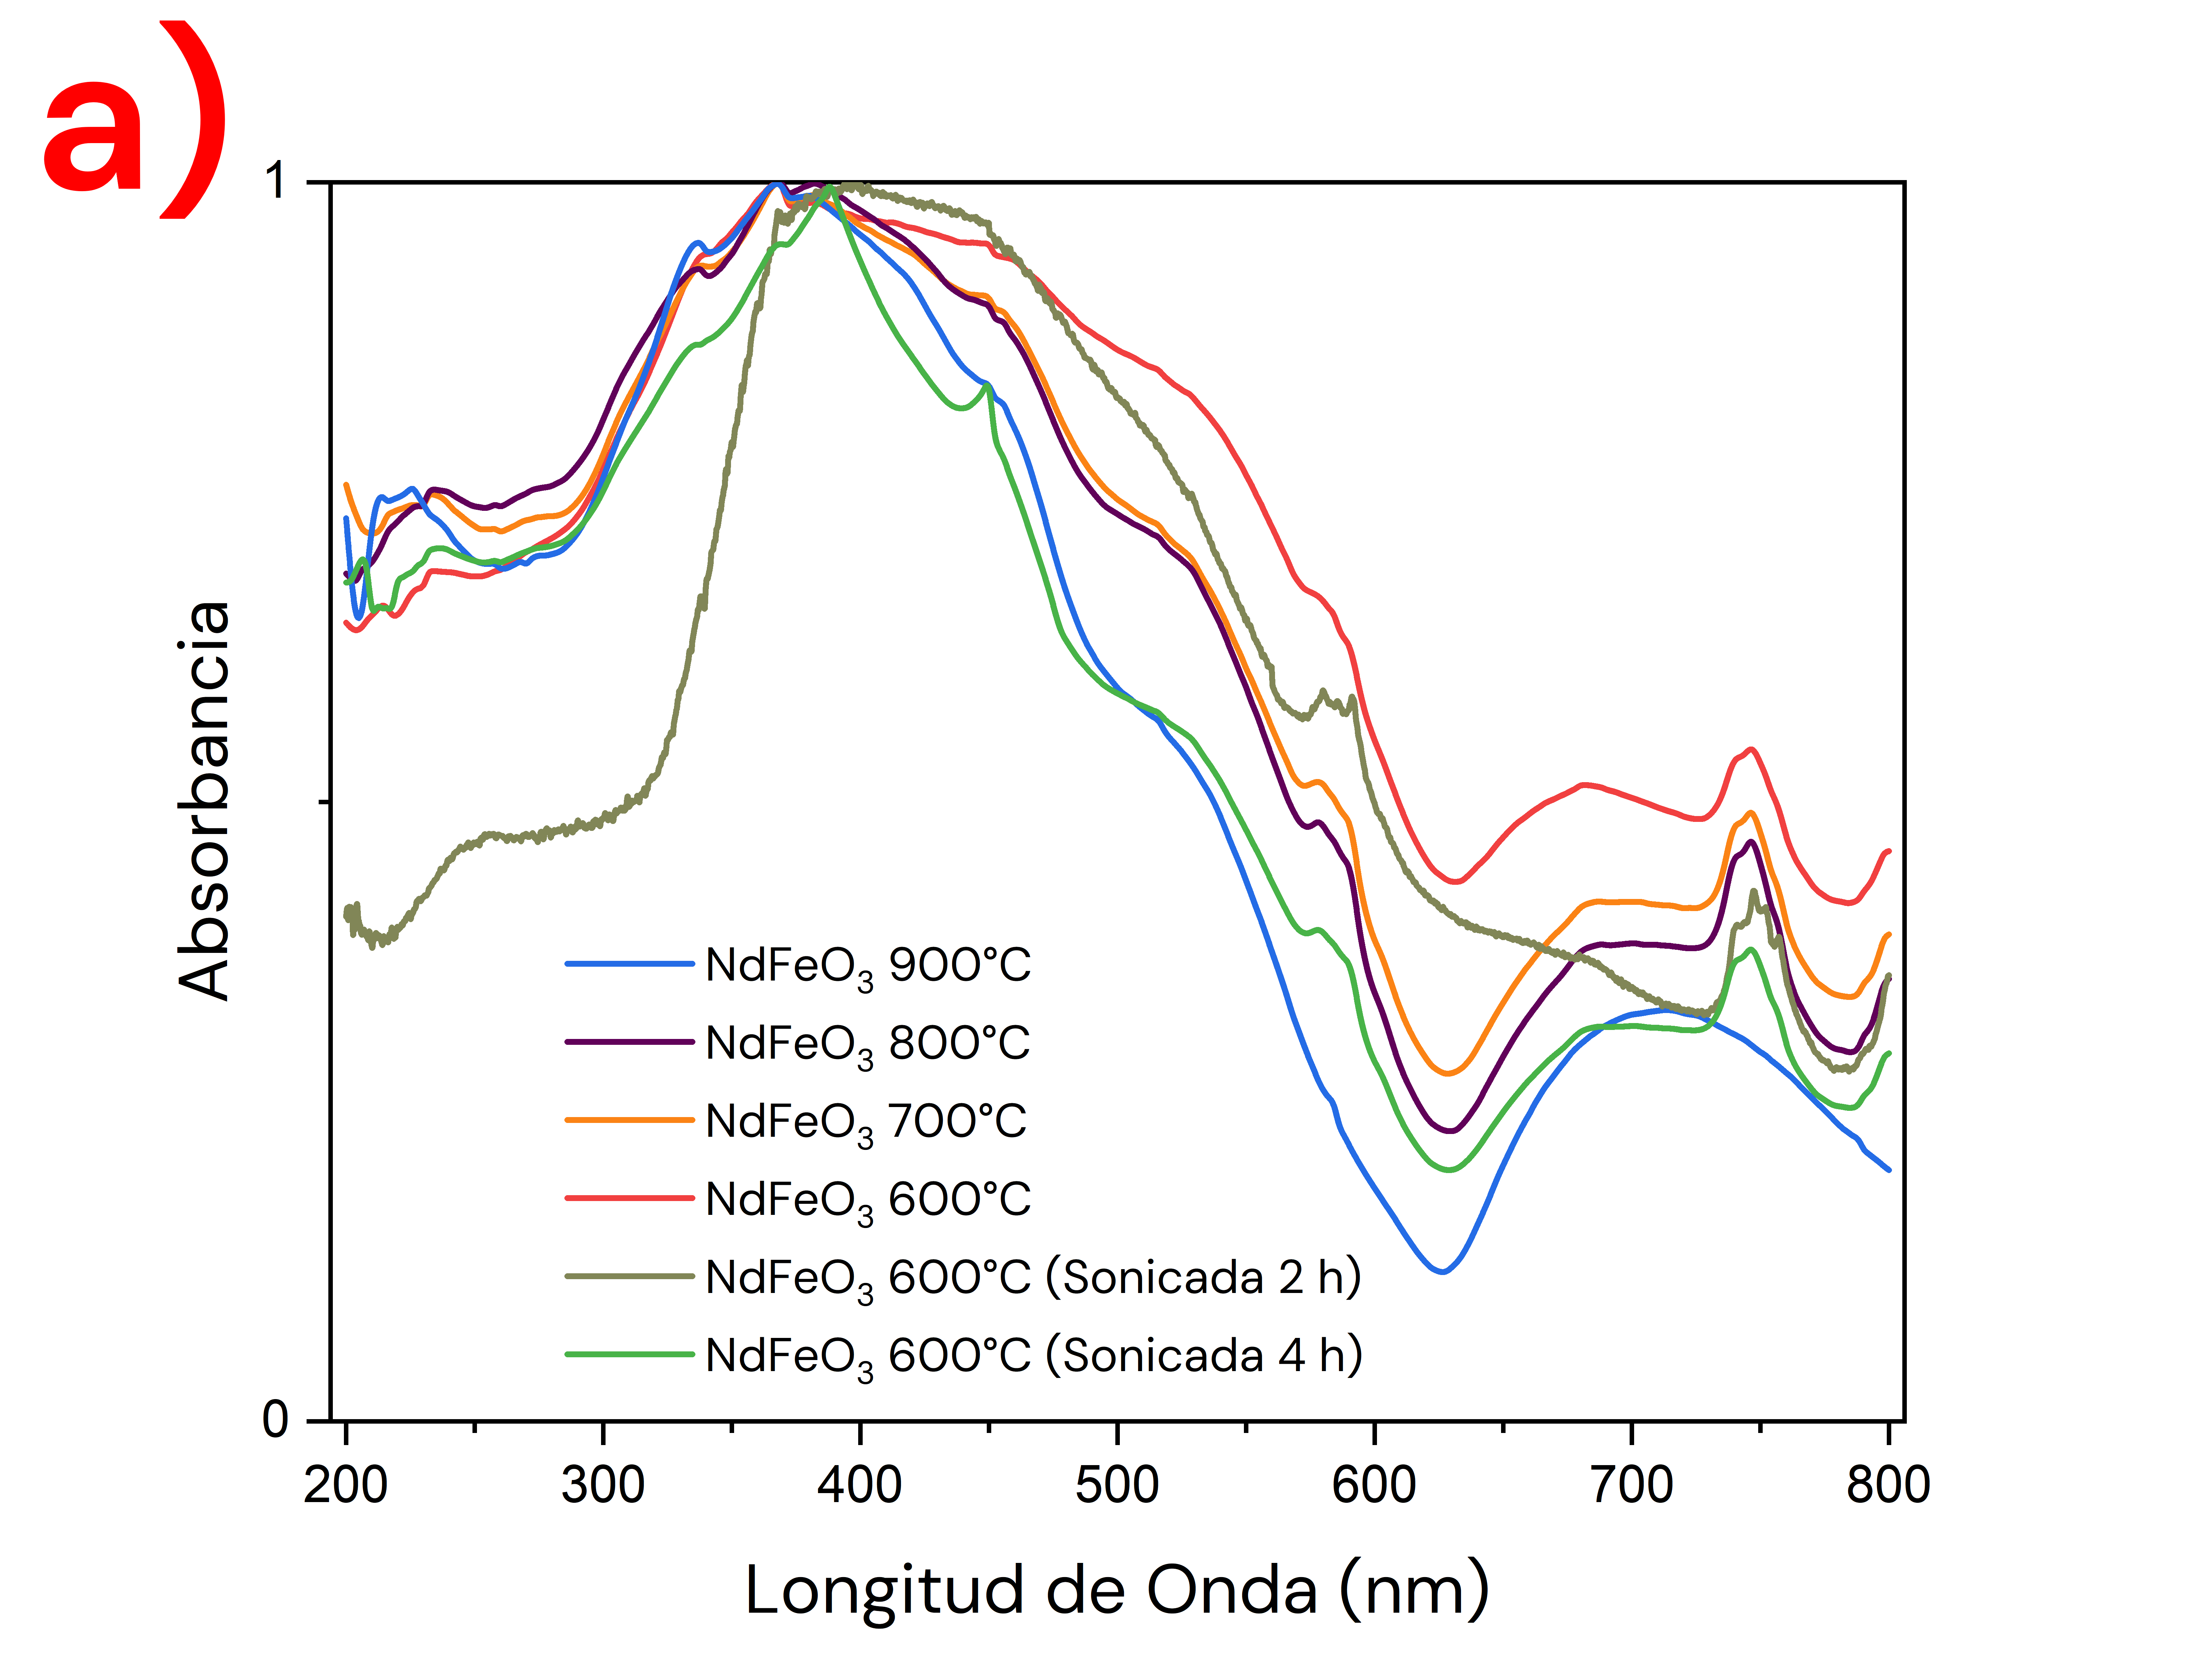
\includegraphics[width=0.7\textwidth]{fig/absorbancianeod.png}
    \caption{Gráficas de la absorbancia contra la longitud de onda para las muestras de \neod{}.}
    \label{fig:absorbresneod}
\end{figure}
Utilizando el método Tauc descrito en la sección \ref{sec:metodotauc} se llegó a los \textit{band gaps} para cada muestra reportados en la tabla \ref{tabla:bandgapsneod}, los cuales se grafican en la figura \ref{fig:bandgapvTneod}.
\begin{table}[H]
    \centering
    \begin{tabular}{|c||c|c|}
        \hline
        Muestra & Temperatura de & \textit{Band Gap} \\
        & calcinación & (eV) \\
        \hline\hline
        \multirow{6}{*}{\rotatebox[origin=c]{90}{\neod{}}} & 600\gradoC{} & 1.84$\pm$0.003 \\
        \cline{2-3}
        & 600\gradoC{}, sonicada 2 h & 2.01$\pm$0.001 \\
        \cline{2-3}
        & 600\gradoC{}, sonicada 4 h & 2.13$\pm$0.009 \\
        \cline{2-3}
        & 700\gradoC{} & 2.05$\pm$0.004 \\
        \cline{2-3}
        & 800\gradoC{} & 2.08$\pm$0.005 \\
        \cline{2-3}
        & 900\gradoC{} & 2.29$\pm$0.004 \\
        \hline
    \end{tabular} 
    \caption{\textit{Band gaps} de las distintas muestras de \neod{} según su temperatura de calcinación.}
    \label{tabla:bandgapsneod}
\end{table}
\begin{figure}[H]
    \centering
    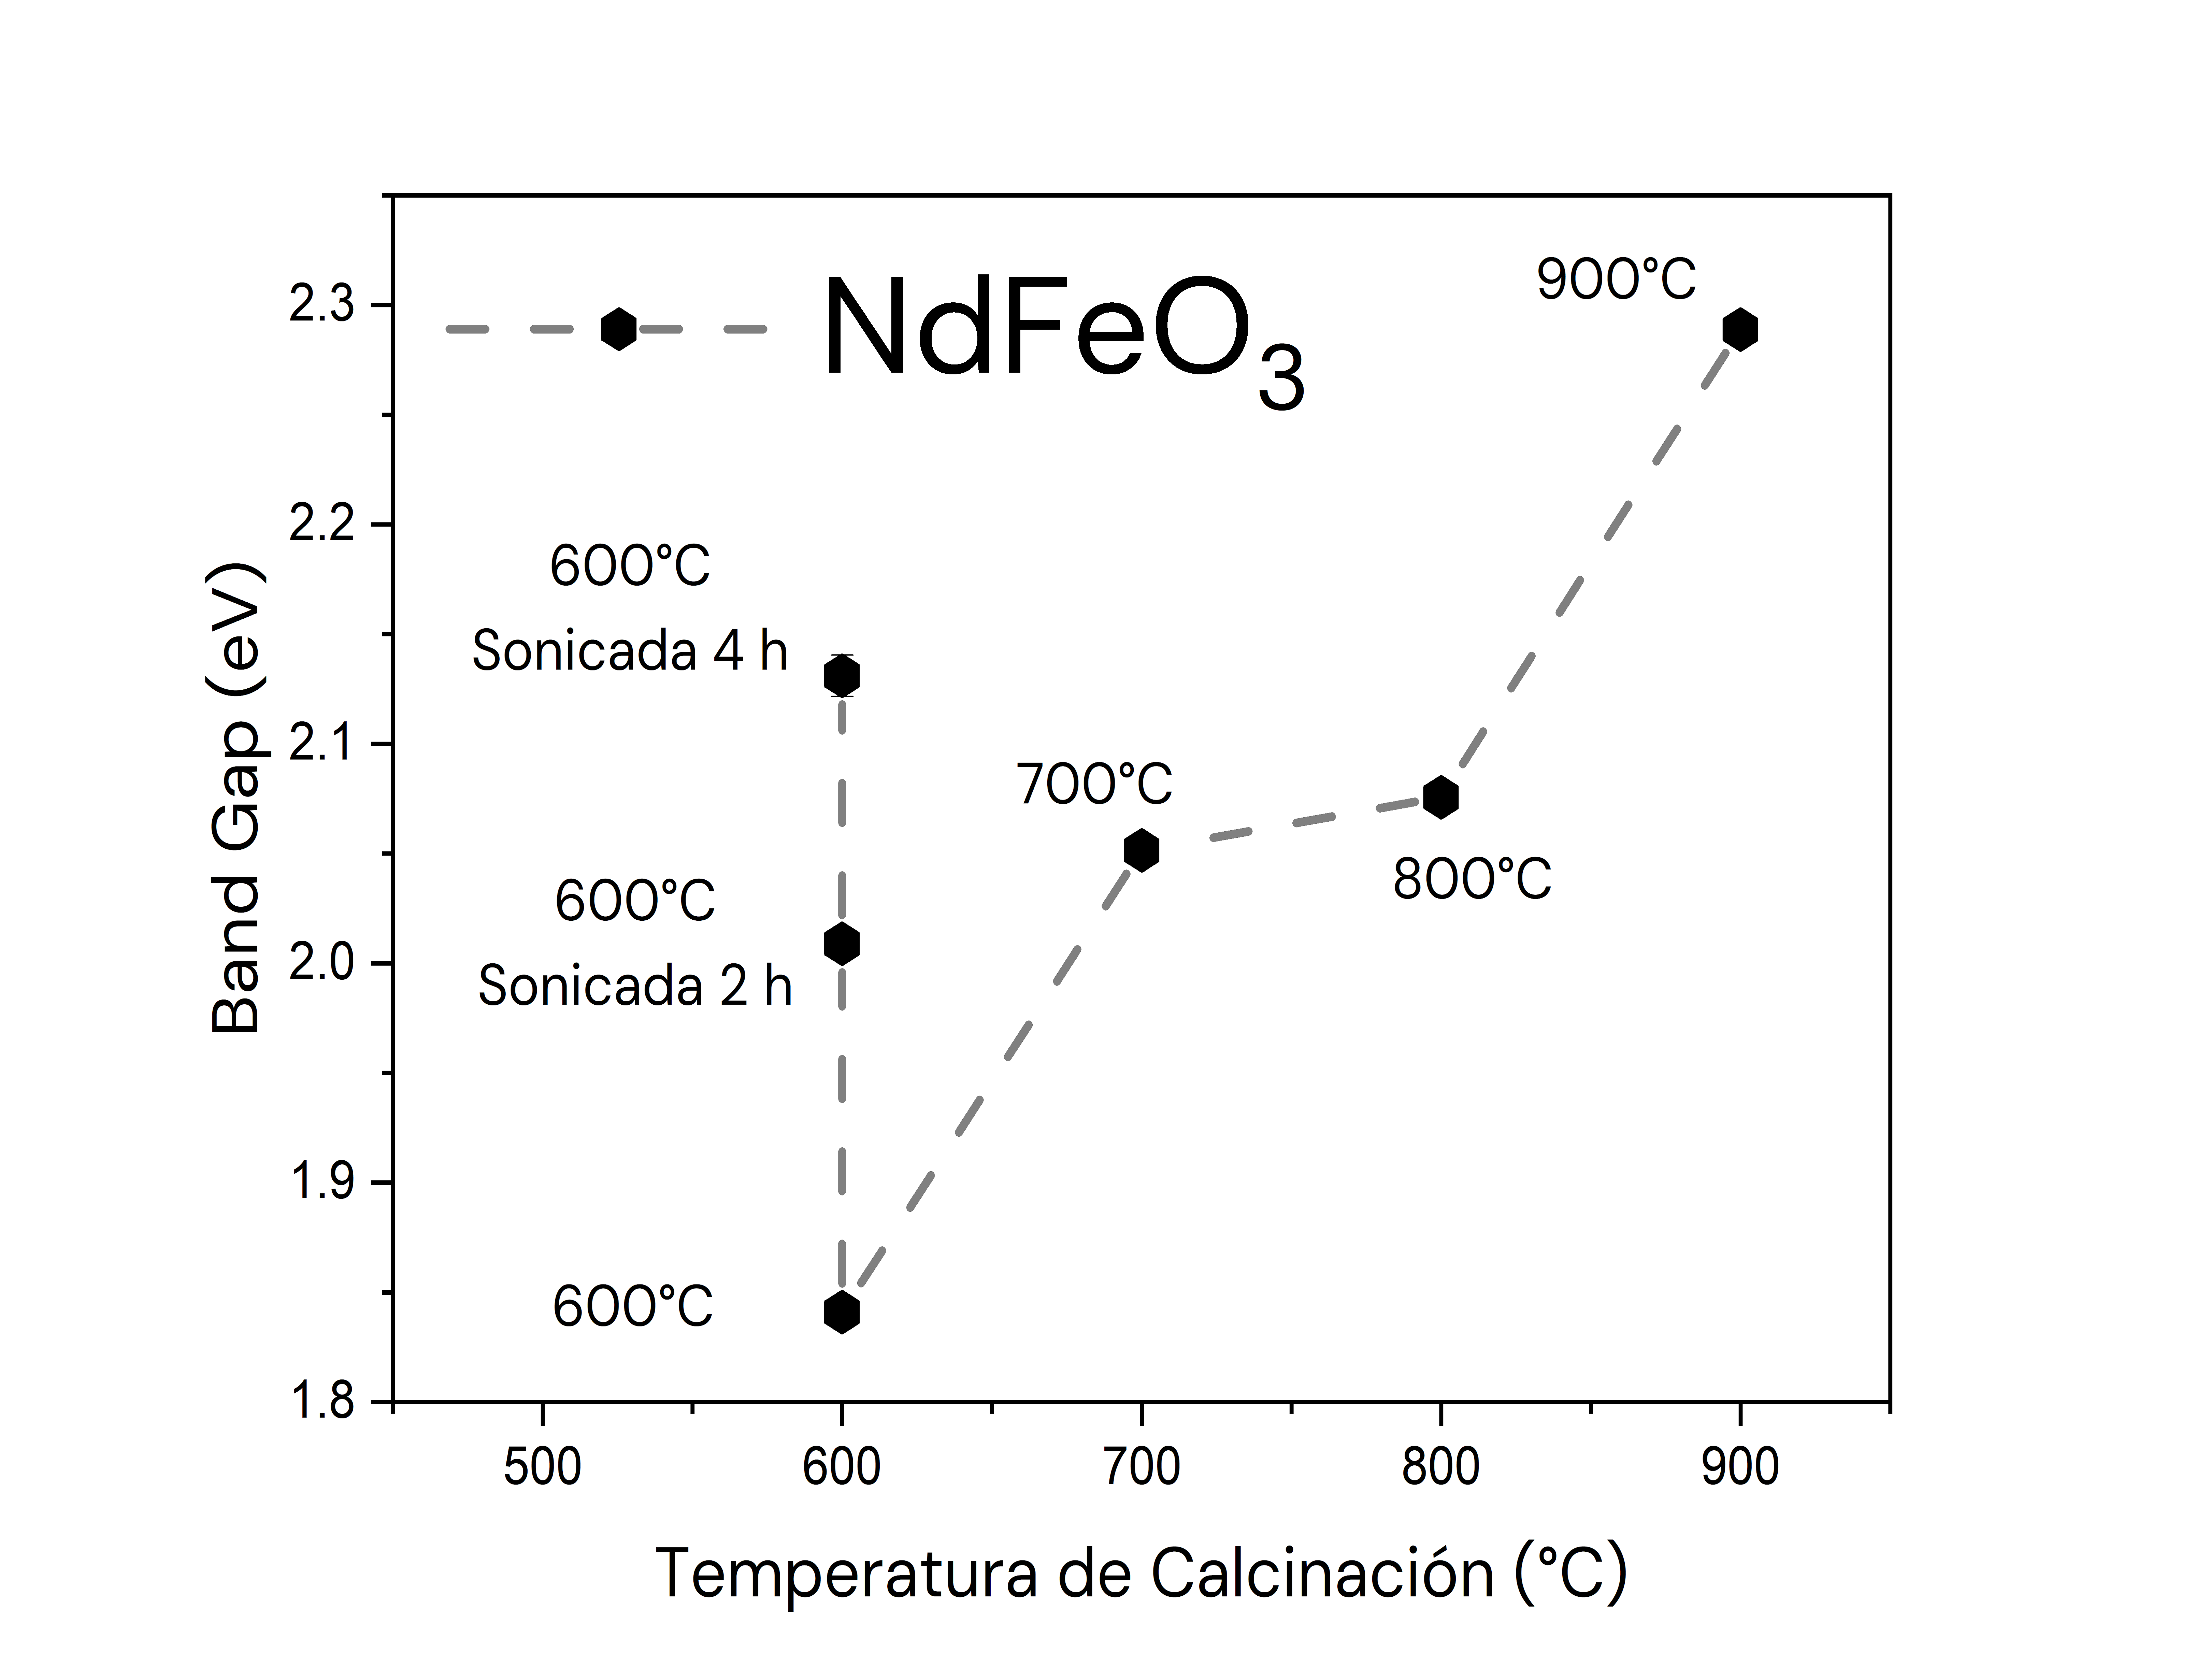
\includegraphics[width=0.7\textwidth]{fig/BGNdFeO3.png}
    \caption{Gráfica del \textit{band gap} de cada muestra de \neod{} según su temperatura de calcinación.}
    \label{fig:bandgapvTneod}
\end{figure}
Se observa que el \textit{band gap} aumenta con la temperatura y el tiempo de sonicación, teniendo un mínimo en la muestra calcinada a menor temperatura y sin sonicar.
\subsubsection{Magnetometría SQUID}
En esta subsección se analizarán los resultados obtenidos para la magnetización como función del campo y de la temperatura, primero para las muestras calcinadas a las dos temperaturas más extremas (aquellas calcinadas a 600\gradoC{} y a 900\gradoC{}) y después se analizará la muestra calcinada a 600\gradoC{} en comparación con la muestra sonicada durante 4 horas y calcinada a la misma temperatura.

En la figura \ref{fig:mvhNd} a) y b) se muestran las curvas $M$ vs $H$ para las muestras calcinadas a 600\gradoC{}  (símbolos vacíos) y a 900\gradoC{}  (símbolos llenos). Estas mediciones fueron tomadas a 5K \ref{fig:mvhNd} a) y a 300K \ref{fig:mvhNd} b). Se puede observar en ambos casos un incremento considerable en las propiedades magnéticas en la muestra calcinada a 900\gradoC{}. Por ejemplo, a 5K la $M_S$ se incrementa a más del doble como se muestra en la tabla \ref{tabla:resmvshneod}.
	
En el caso de las mediciones llevadas a cabo a 300K (\ref{fig:mvhNd} b)), vemos que la muestra calcinada a 900\gradoC, presenta ferromagnetismo débil ya que hay un bucle de histéresis casi lineal. Sin embargo se observa un campo coercitivo pequeño ligeramente antisimétrico. Este comportamiento ferromagnético débil puede explicarse gracias a las subredes \ce{Fe^{3+}} alineadas antiferromagnéticamente pero que presentan inclinación conocida como (\textit{canting}). En contraste la muestra calcinada a 600\gradoC{}, muestra ciclos de histéresis saturados tanto a 5K como a 300K, una magnetización de saturación ($M_S$) con valores más altos, una magnetización de remanencia pequeña ($M_R$) así como campos coercitivos simétricos ($H_C$).
	
En este tipo de muestras el comportamiento magnético se origina en la existencia de iones magnéticos Fe y R, sus interacciones mutuas y las peculiaridades de la anisotropía de un solo ion \cite{Zhou2014} En \ce{RFeO3} cada ion Fe está rodeado por seis iones O que forman un octaedro \ce{O6}, donde O es el vértice común de los dos octaedros adyacentes que actúan como intermediario de una interacción de superintercambio \cite{coey2010magnetism}. La transición del estado antiferromagnético al estado paramagnético caracterizado por la temperatura de Néel ($T_{N1}$) generalmente ocurre a altas temperaturas (generalmente por encima de 600\gradoC{}) \cite{Wang2019}.

Sin embargo existen ordenamientos ferromagnéticos débiles por debajo de $T_{N1}$ \cite{Bouziane2005}. Debido al mecanismo  Dzyaloshinskii-Moriya, el momento magnético del Fe no es totalmente antiparalelo al del Fe más cercano, sino que normalmente se inclina en un pequeño ángulo \cite{Dzyaloshinsky1958}. Por lo tanto, algunos \ce{RFeO3} poseen un ferromagnetismo débil como resultado de la inclinación del espín con respecto al ordenamiento antiferromagnético ideal de dos subredes que es el caso de las muestras que hemos mostrado en la figura \ref{fig:mvhNd}.

\begin{figure}[H]
    \centering
    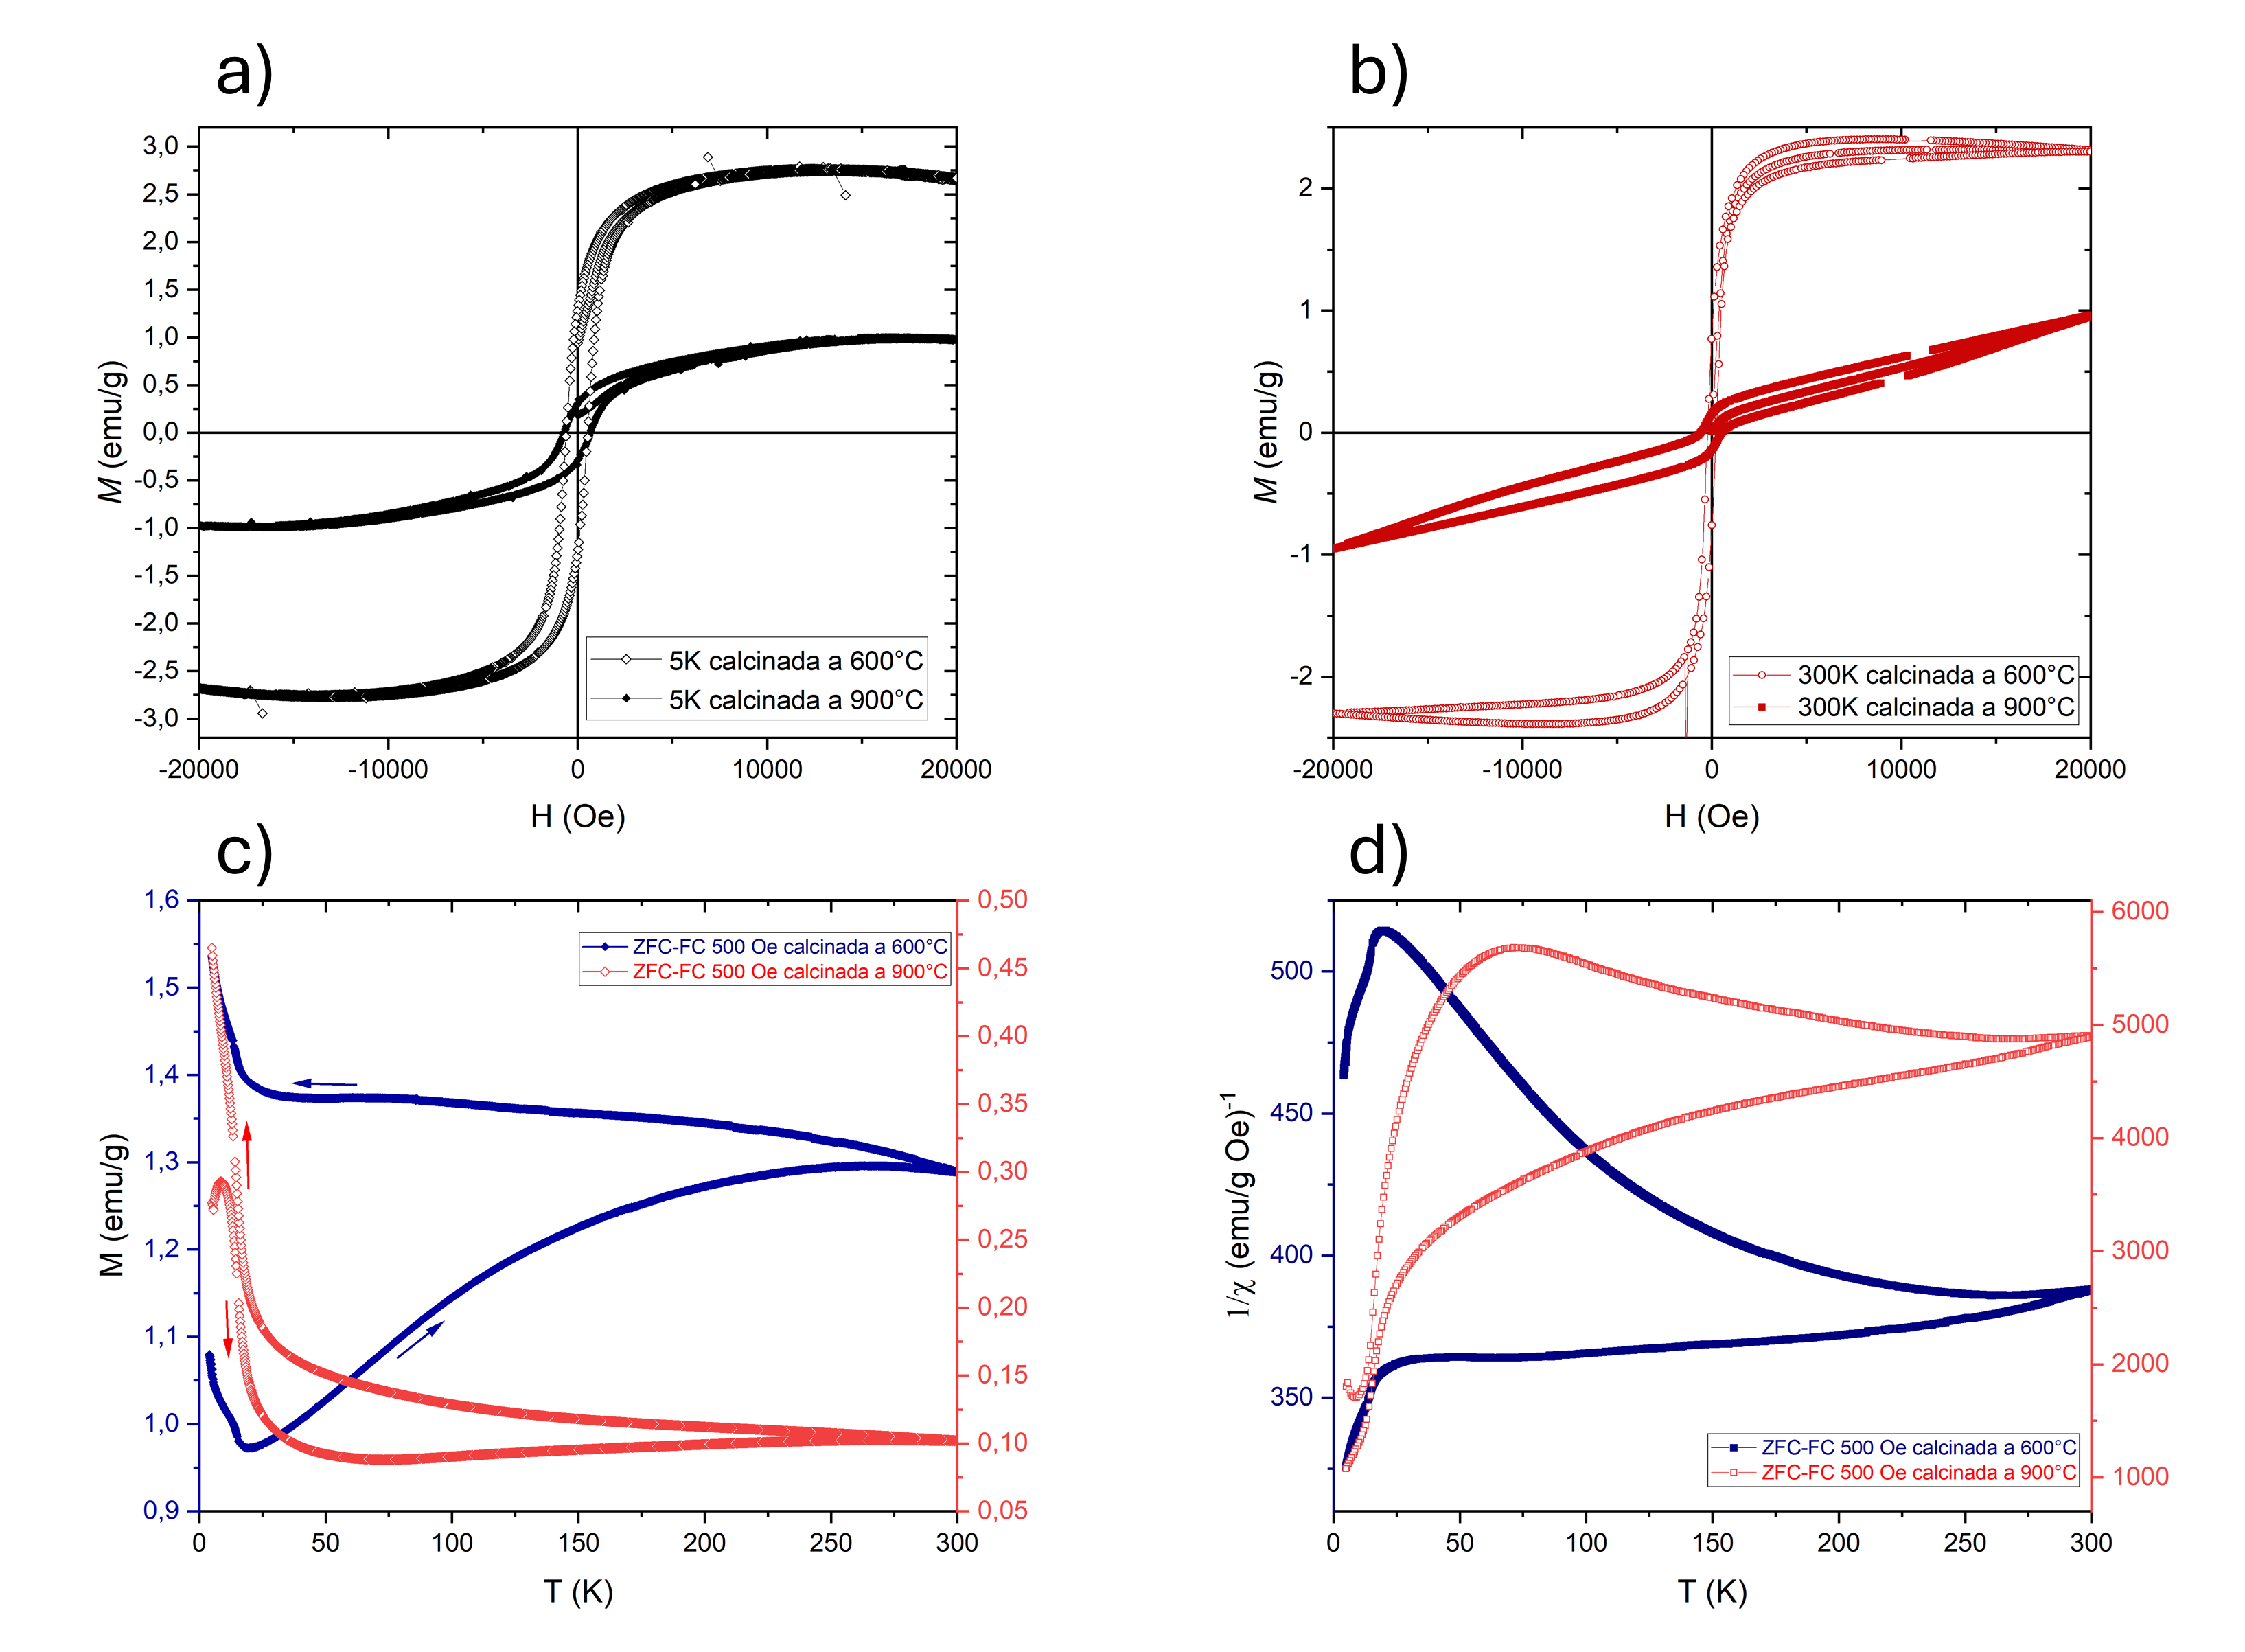
\includegraphics[width=0.9\textwidth]{fig/Magnetometria_NdFeO3_T_calc.png}
    \caption{Magnetometría de las muestras \neod{} calcinadas a 600\gradoC{} y a 900\gradoC{}: a) Curvas $M$ vs $H$ a 5K para las muestras calcinadas a 600\gradoC{}  (diamantes vacíos negros) y a 900\gradoC{} (diamantes llenos negros), b) Curvas $M$ vs $H$ a 300K para las muestras calcinadas a 600\gradoC{}  (círculos vacíos rojos) y a 900\gradoC{} (cuadrados llenos rojos),  c) $M$ vs $T$ FC-ZFC a 500 Oe para la muestra calcinada a 600\gradoC{} (diamantes azules llenos) y a 900\gradoC{} (diamantes rojos vacíos) d) $\chi^{-1}$ vs $T$ a 500 Oe a 500 Oe para la muestra calcinada a 600\gradoC{} (diamantes azules llenos) y a 900\gradoC{} (diamantes rojos vacíos).}
    \label{fig:mvhNd}
\end{figure}

En la figura \ref{fig:mvhNd} c) se muestran las curvas $M$ vs $T$ enfriadas sin campo (ZFC) y con campo (FC) con un campo externo de 500 Oe. La curva roja muestra el comportamiento de $M$ para la muestra calcinada a 900\gradoC{}.  El repentino aumento de la pendiente por debajo de 25 K indica que los espines \ce{Nd^{3+}} se ordenan en el campo de intercambio de los espines \ce{Fe^{3+}},  $M(T)$ continúa aumentando a bajas temperaturas. Sin embargo, cuando la misma muestra es enfriada en en ausencia de campo (ZFC), se observa que por $M(T)$ tiene un máximo en $\sim$ 8 K por debajo del cual $M$ es decreciente, lo cual indica una alineación de espines predominantemente antiparalela. Esto también se muestra en la curva $\chi^{-1}$ vs $T$ en la figura \ref{fig:mvhNd} d) donde la curva roja muestra un mínimo alrededor de 8 K. En contraste la muestra calcinada a 600\gradoC{} (curva azul en las figuras \ref{fig:mvhNd} c) y d)) solamente presenta la presencia de ferromagnetismo débil y un ligero aumento de $M(T)$ por debajo de 25K posiblemente por la alineación paralela de los iones \ce{Nd^{3+}}.

Por otro lado, la muestra calcinada a 600\gradoC{} que fue sometida a un proceso de sonicación durante 4 h, no presenta cambios significativos después del proceso de sonicación como se muestra en la figura \ref{fig:mvhNdsonic}. En la tabla \ref{tabla:resmvshneod}, puede observarse que los valores de $M_S$, $M_R$ y $H_c$ no presentan una variación significativa ni a 5 K ni a 300 K (figura \ref{fig:mvhNdsonic} a) y b)). De la misma forma, el comportamiento de $M$ vs $T$ y de $\chi^{-1}$ vs $T$ para las muestras enfriadas con campo y sin campo (FC-ZFC) (figura \ref{fig:mvhNdsonic} c) y d) respectivamente), presentan comportamientos muy similares para la muestra sonicada y sin sonicar. Estos pueden explicarse debido a que la reducción de tamaño de la partícula no es comparable al cambio de tamaño del cristal al variar la temperatura de calcinación.

\begin{figure}[H]
	\centering
	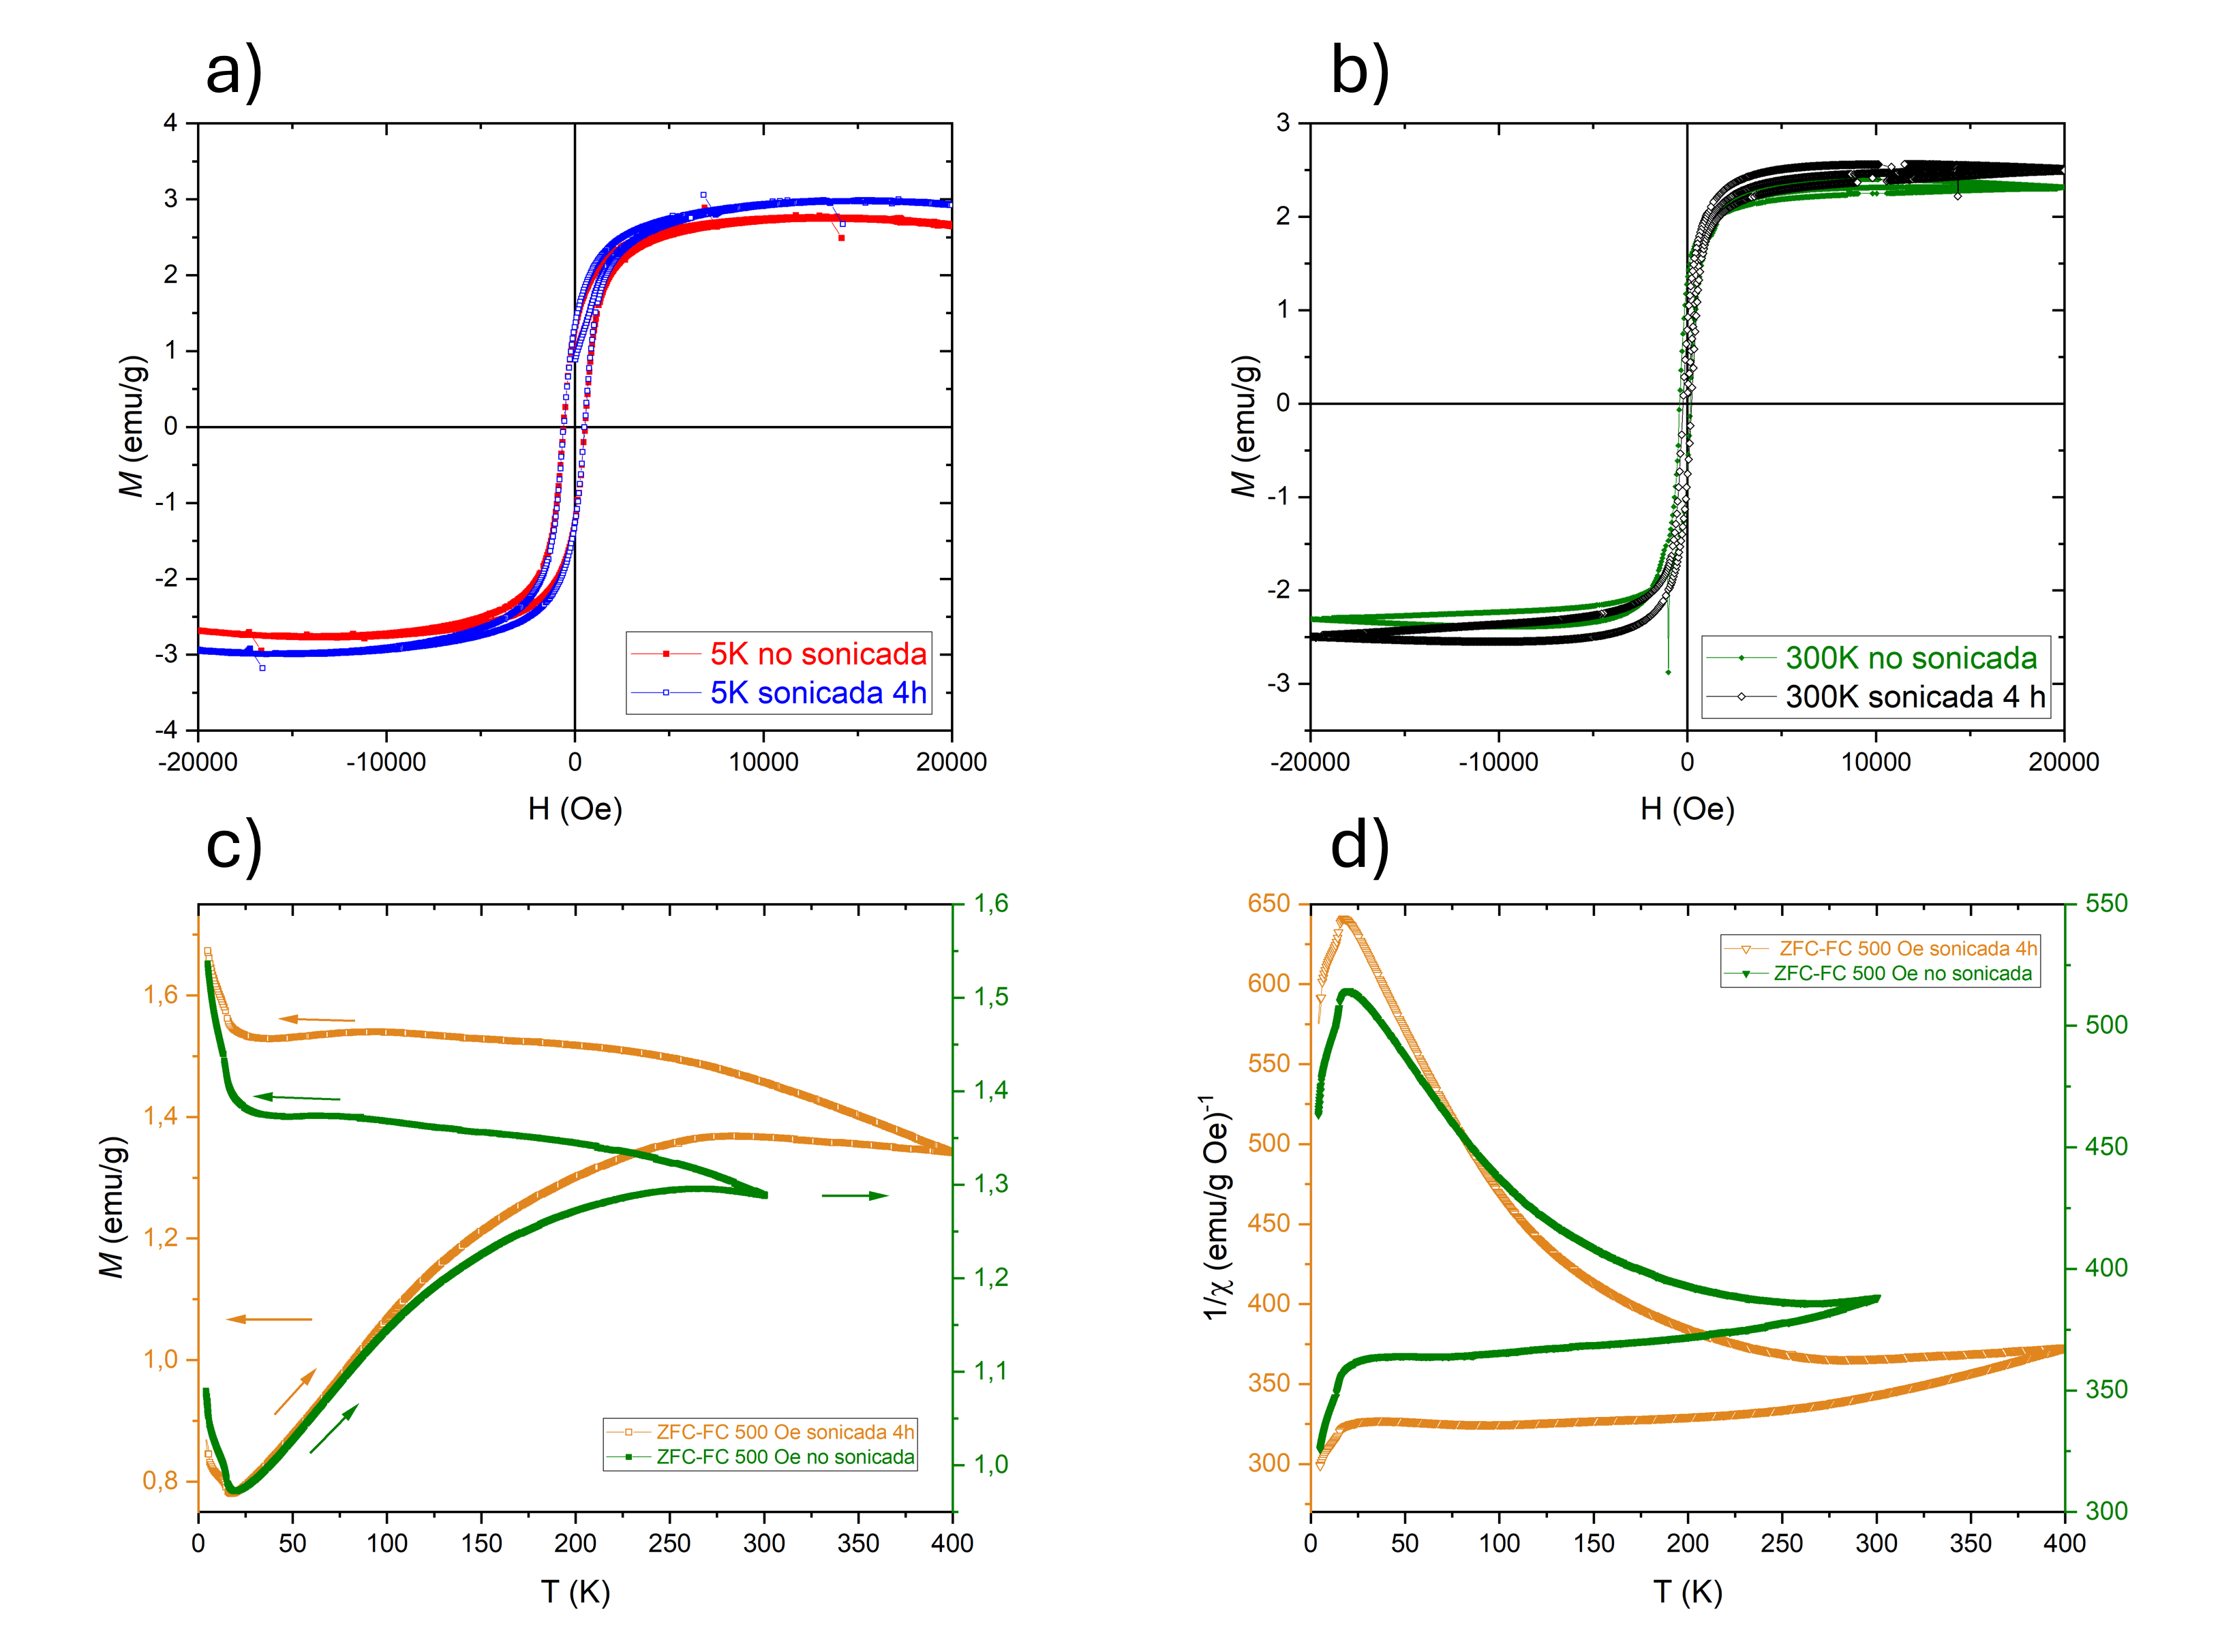
\includegraphics[width=0.9\textwidth]{fig/Magnetometria_NdFeO3_sonic.png}
	\caption{Magnetometría de las muestras \neod{} calcinadas a 600\gradoC{} sin sonicar y sonicada durante 4h: (a) Curvas $M$ vs $H$ a 5 K para las muestras sin sonicar  (cuadrados llenos rojos) y sonicada (cuadrados vacíos azules), (b) Curvas $M$ vs $H$ a 300 K para las muestras para las muestras sin sonicar  (diamantes llenos verdes) y sonicada (diamantes negros vacíos), (c) $M$ vs $T$ FC-ZFC a 500 Oe para la muestra sin sonicar (cuadrados verdes llenos) y no sonicada (cuadrados naranjas vacíos)(d) $\chi^{-1}$ vs $T$ a 500 Oe para la muestra sin sonicar (cuadrados verdes llenos) y no sonicada (cuadrados naranjas vacíos).}
	\label{fig:mvhNdsonic}
\end{figure}

A continuación se reportan los valores obtenidos para $M_r$, $M_s$ y $H_c$ para la muestra calcinada a 600\gradoC{} sonicada y sin sonicar, así como para la muestra calcinada a 900\gradoC{}:

\begin{table}[H]
    \centering
    \begin{tabular}{|c||c|c|c|}
        \hline 
        Muestra & $M_s$ (emu/g) & $M_r$ (emu/g) & $H_c$ (Oe) \\
        \hline
        \hline
        \multicolumn{4}{|c|}{$T=5$ K} \\
        \hline
        \neod{} (600\gradoC{}) sin sonicar & 2.83$\pm$0.006 & 1.74$\pm$0.024 & 523.71$\pm$23.818 \\
        \hline
        \neod{} (600\gradoC{}) sonicada 4 h & 2.63$\pm$0.011 & 1.44$\pm$0.032 & 219.61$\pm$17.736 \\
        \hline
        \neod{} (900\gradoC{}) & 0.91$\pm$0.005 & 0.26$\pm$0.006 & 869.08$\pm$17.560 \\
        \hline
        \multicolumn{4}{|c|}{$T=300$ K} \\
        \hline 
        Muestra & $M_s$ (emu/g) & $M_r$ (emu/g) & $H_c$ (Oe) \\
        \hline
        \hline
        \neod{} (600\gradoC{}) sin sonicar & 2.18$\pm$0.001 & 0.83$\pm$0.012 & 163.64$\pm$74.669 \\
        \hline
        \neod{} (600\gradoC{}) sonicada 4 h & 2.34$\pm$0.001 & 0.92$\pm$0.039 & 153.87$\pm$28.621 \\
        \hline
        \neod{} (900\gradoC{}) & 0.25$\pm$0.00 & 0.14$\pm$0.003 & 688.92$\pm$16.033 \\
        \hline
        \end{tabular} 
    \caption{Valores de $M_s$, $M_r$ y $H_c$ obtenidos para las muestras de \neod{}.}
    \label{tabla:resmvshneod}
\end{table}
\subsubsection{Curvas de polarización}
En las figuras \ref{fig:nd100v} y \ref{fig:nd2000v} se reportan las curvas $P$ vs $E$ de las muestras de \neod{} sinterizadas con un voltaje aplicado máximo de $V_{max}=$ 100 y 2000 V respectivamente.
\begin{figure}[H]
    \centering
    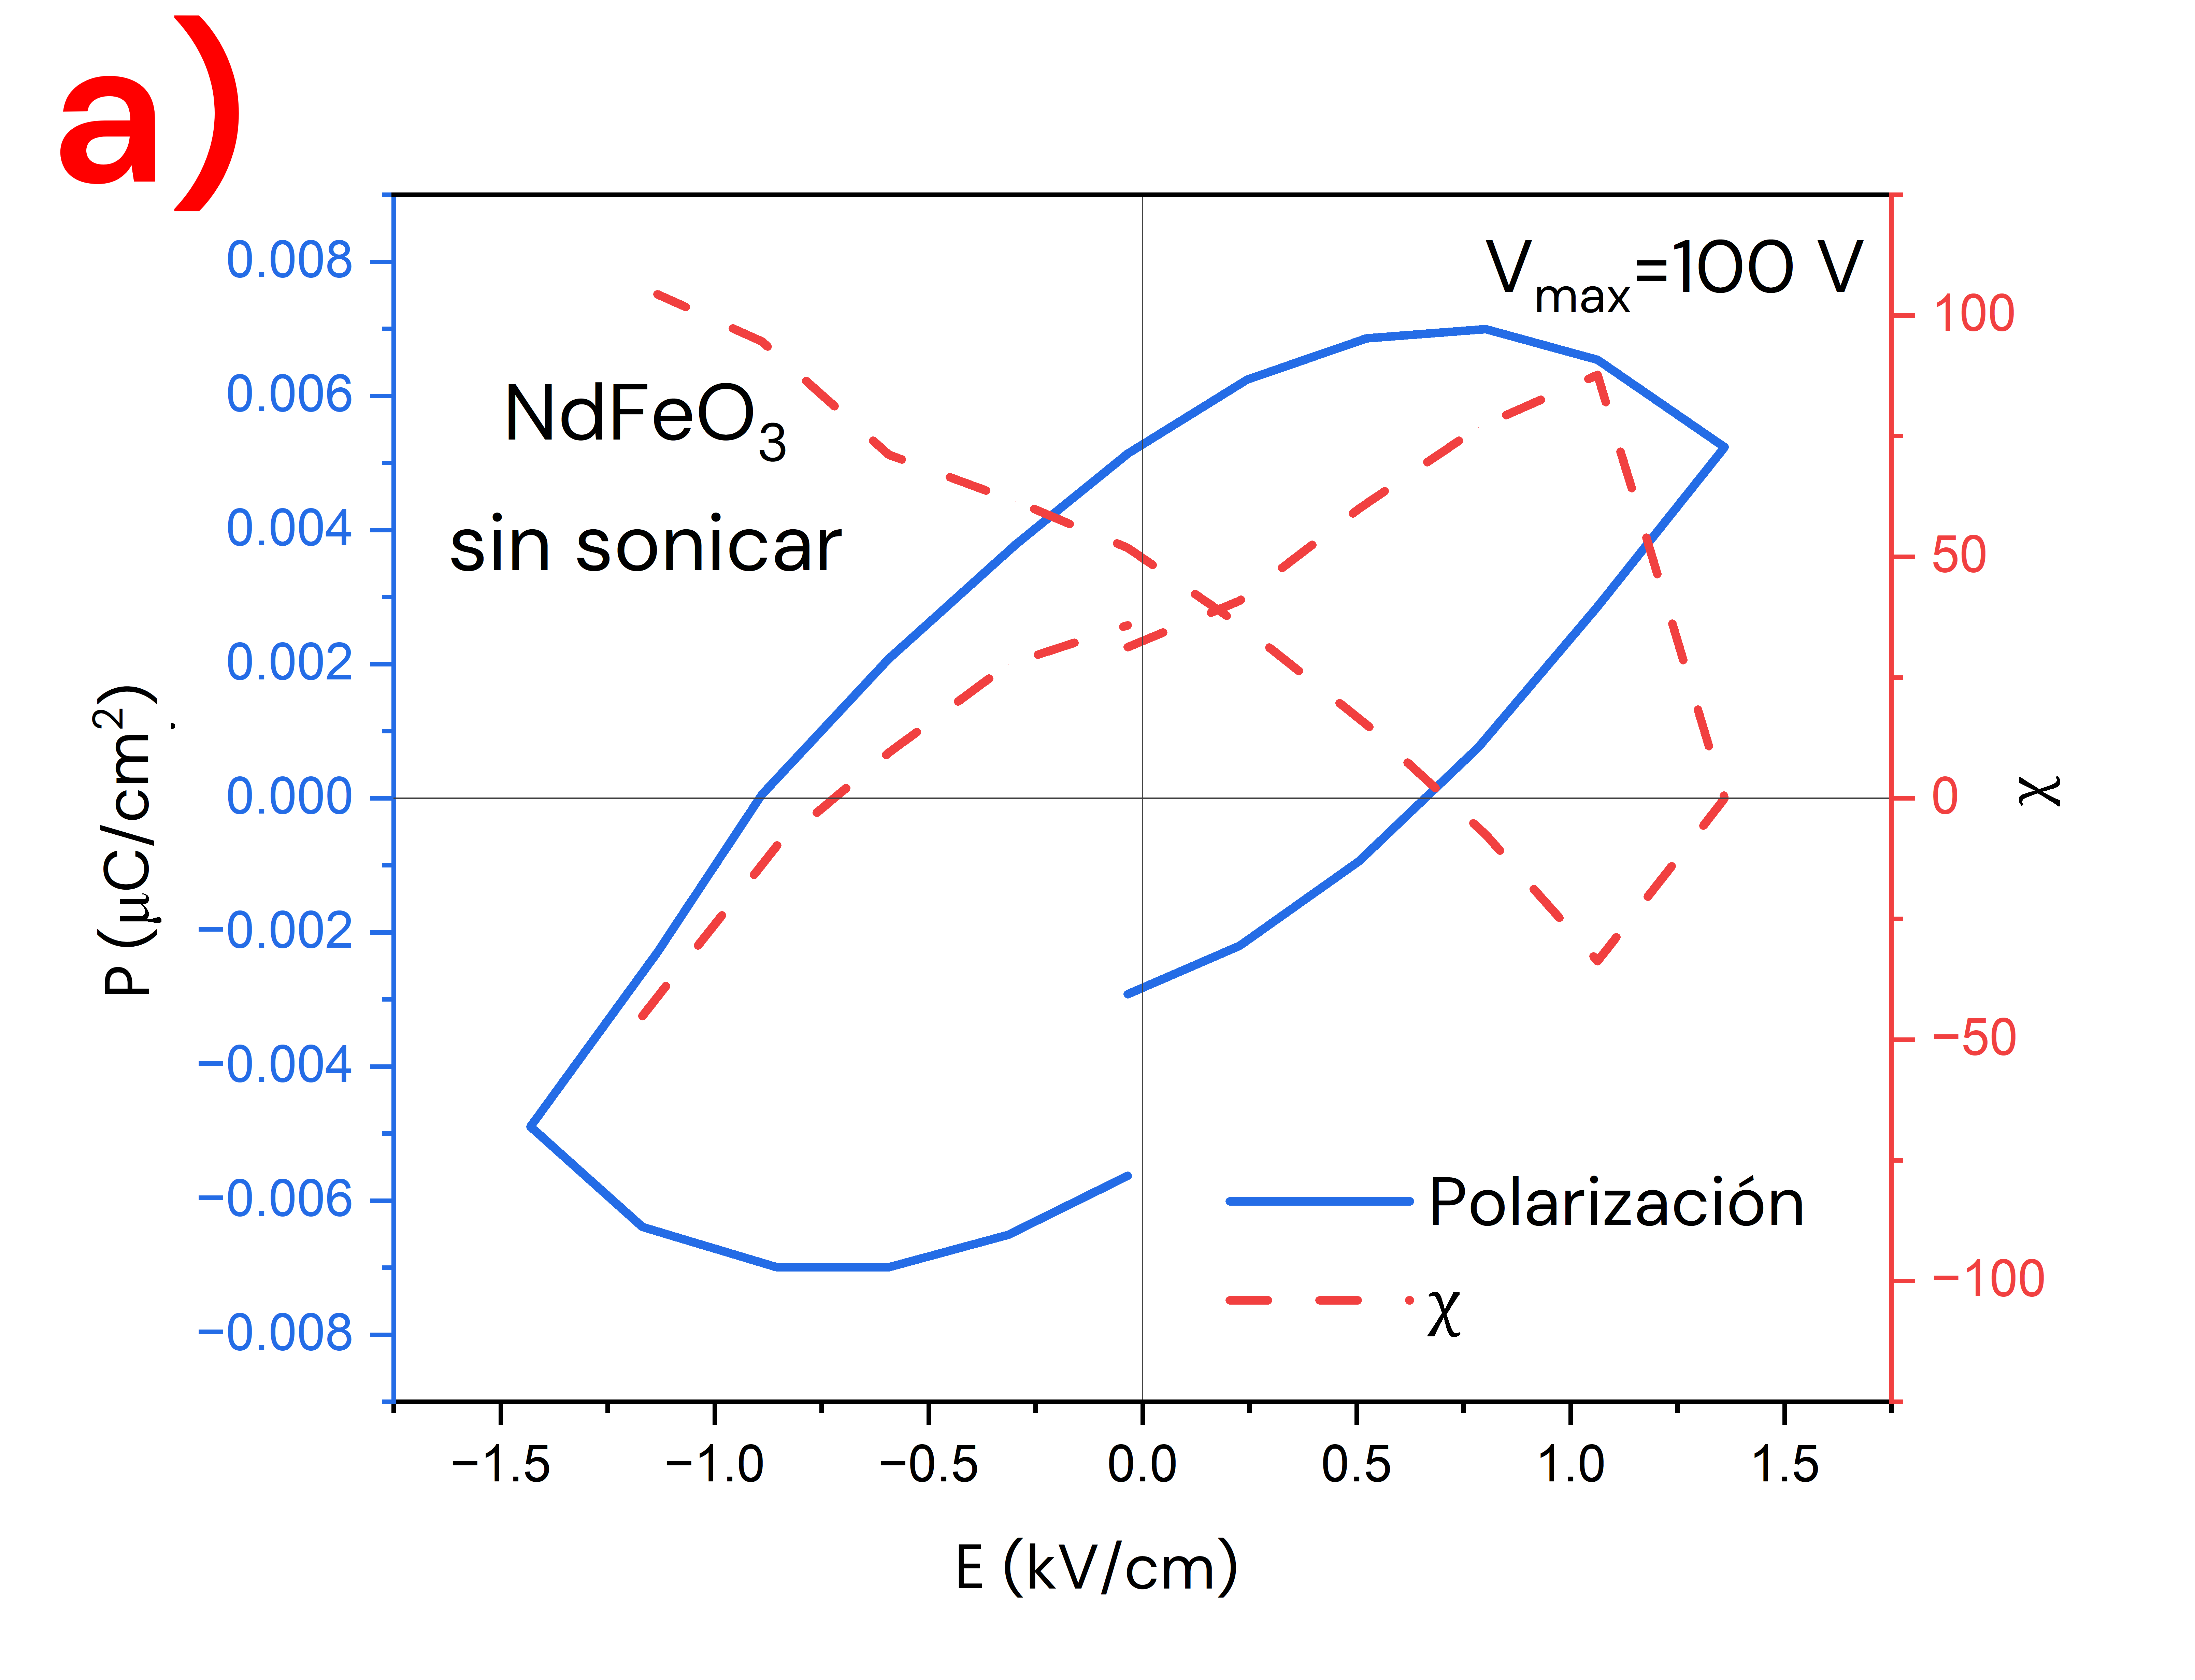
\includegraphics[width=0.45\textwidth]{fig/PENdFeO3100V.png}
    \quad
    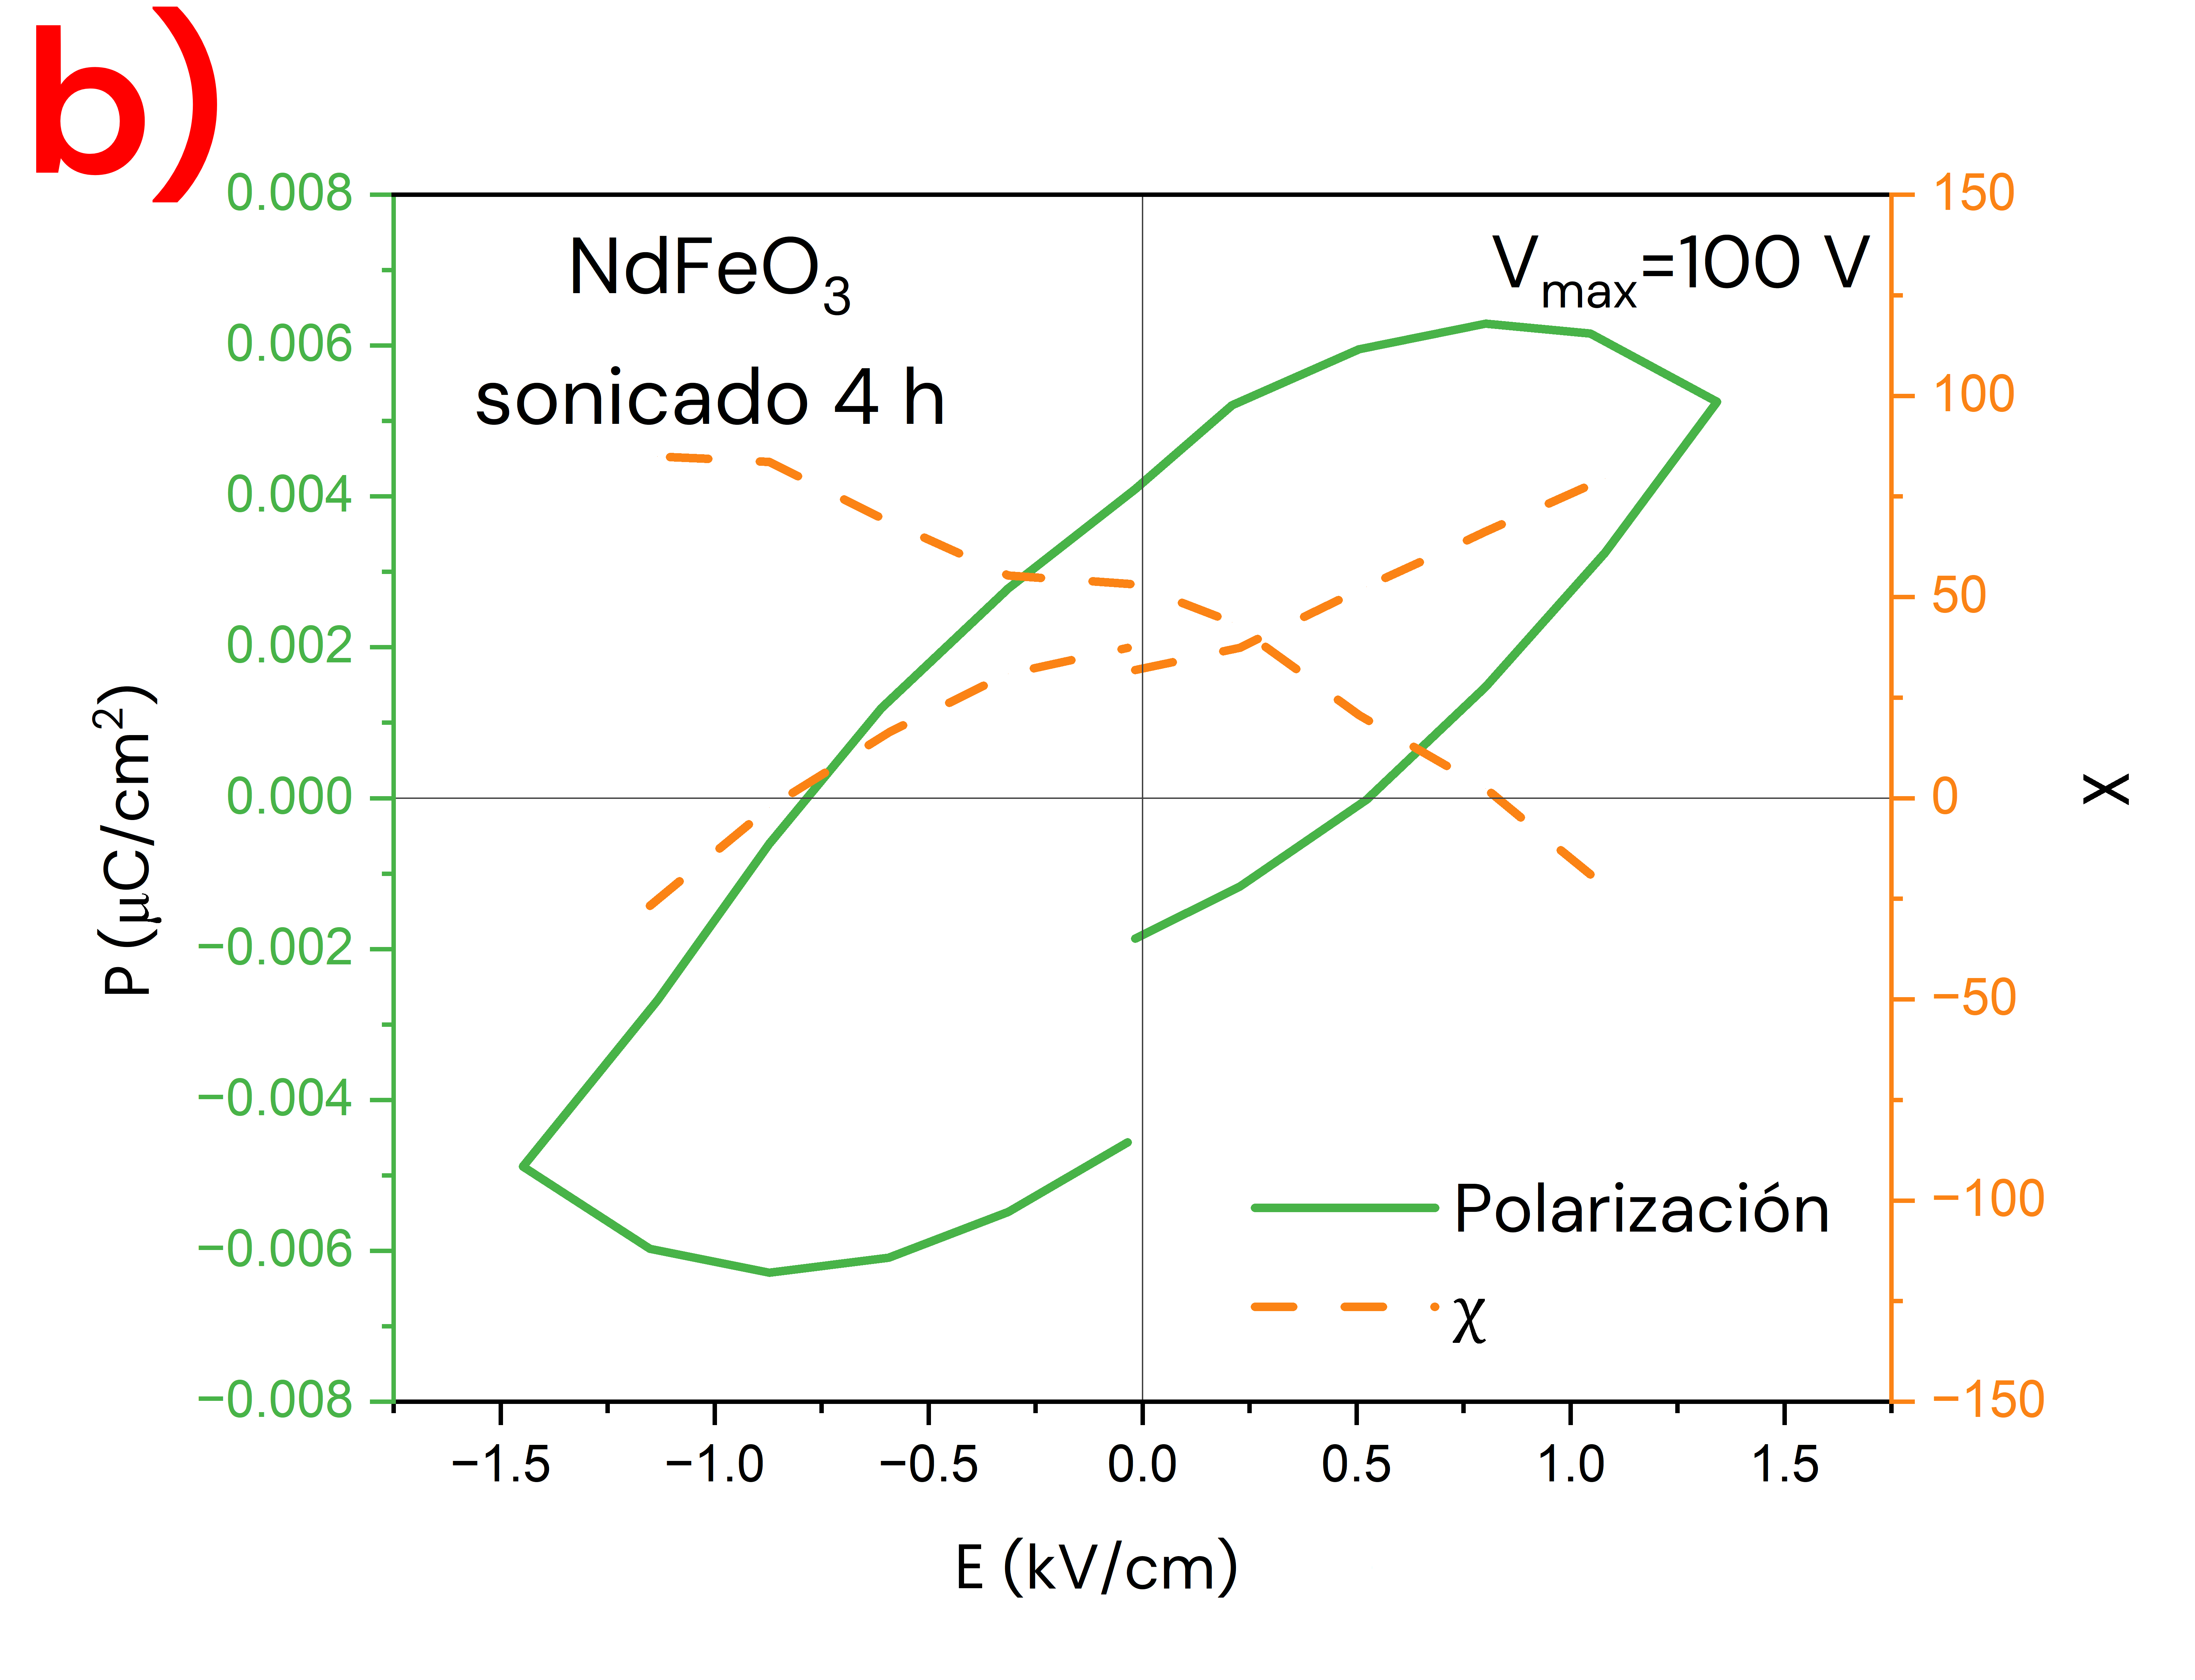
\includegraphics[width=0.45\textwidth]{fig/PENdFeO3-S100V.png}
    \caption{Curvas $P$ contra $E$ (eje izquierdo) y $\chi$ contra $E$ (eje derecho) con $V_\text{max}=100$ V de las muestras de \neod{}: a) sin sonicar y b) sonicada 4 h.}
    \label{fig:nd100v}
\end{figure}
\begin{figure}[H]
    \centering
    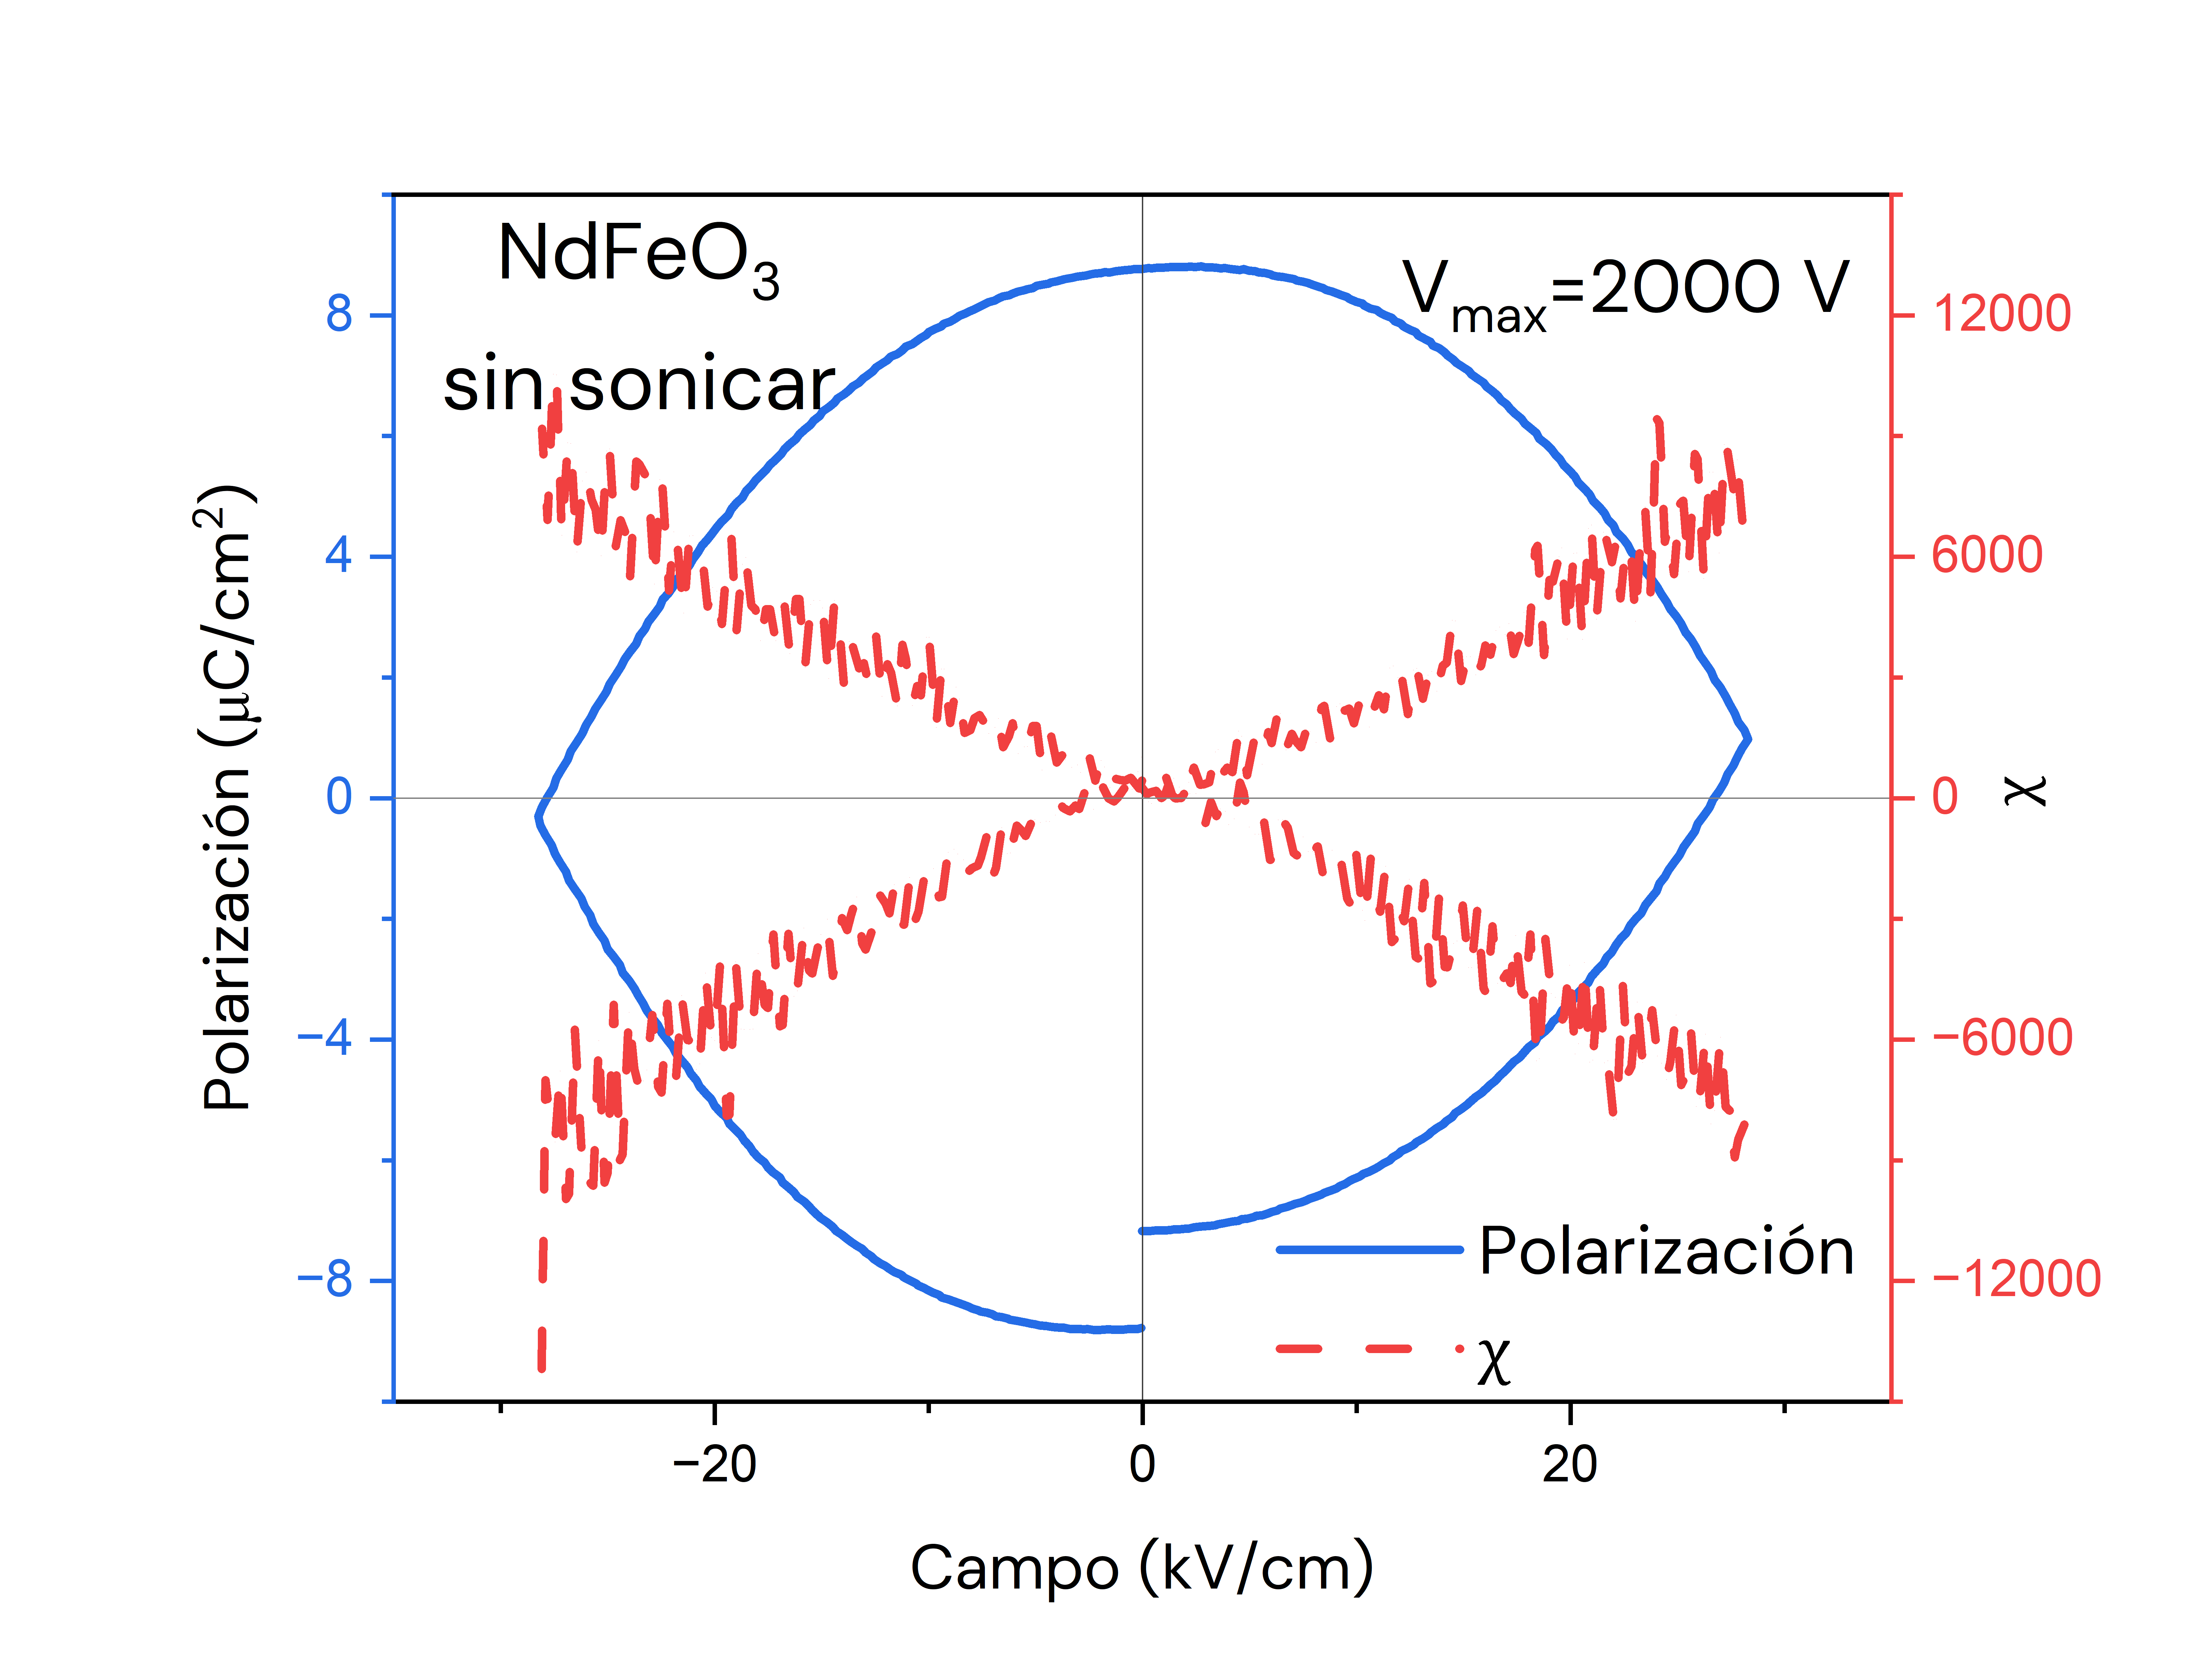
\includegraphics[width=0.45\textwidth]{fig/PENdFeO32000V.png}
    \quad
    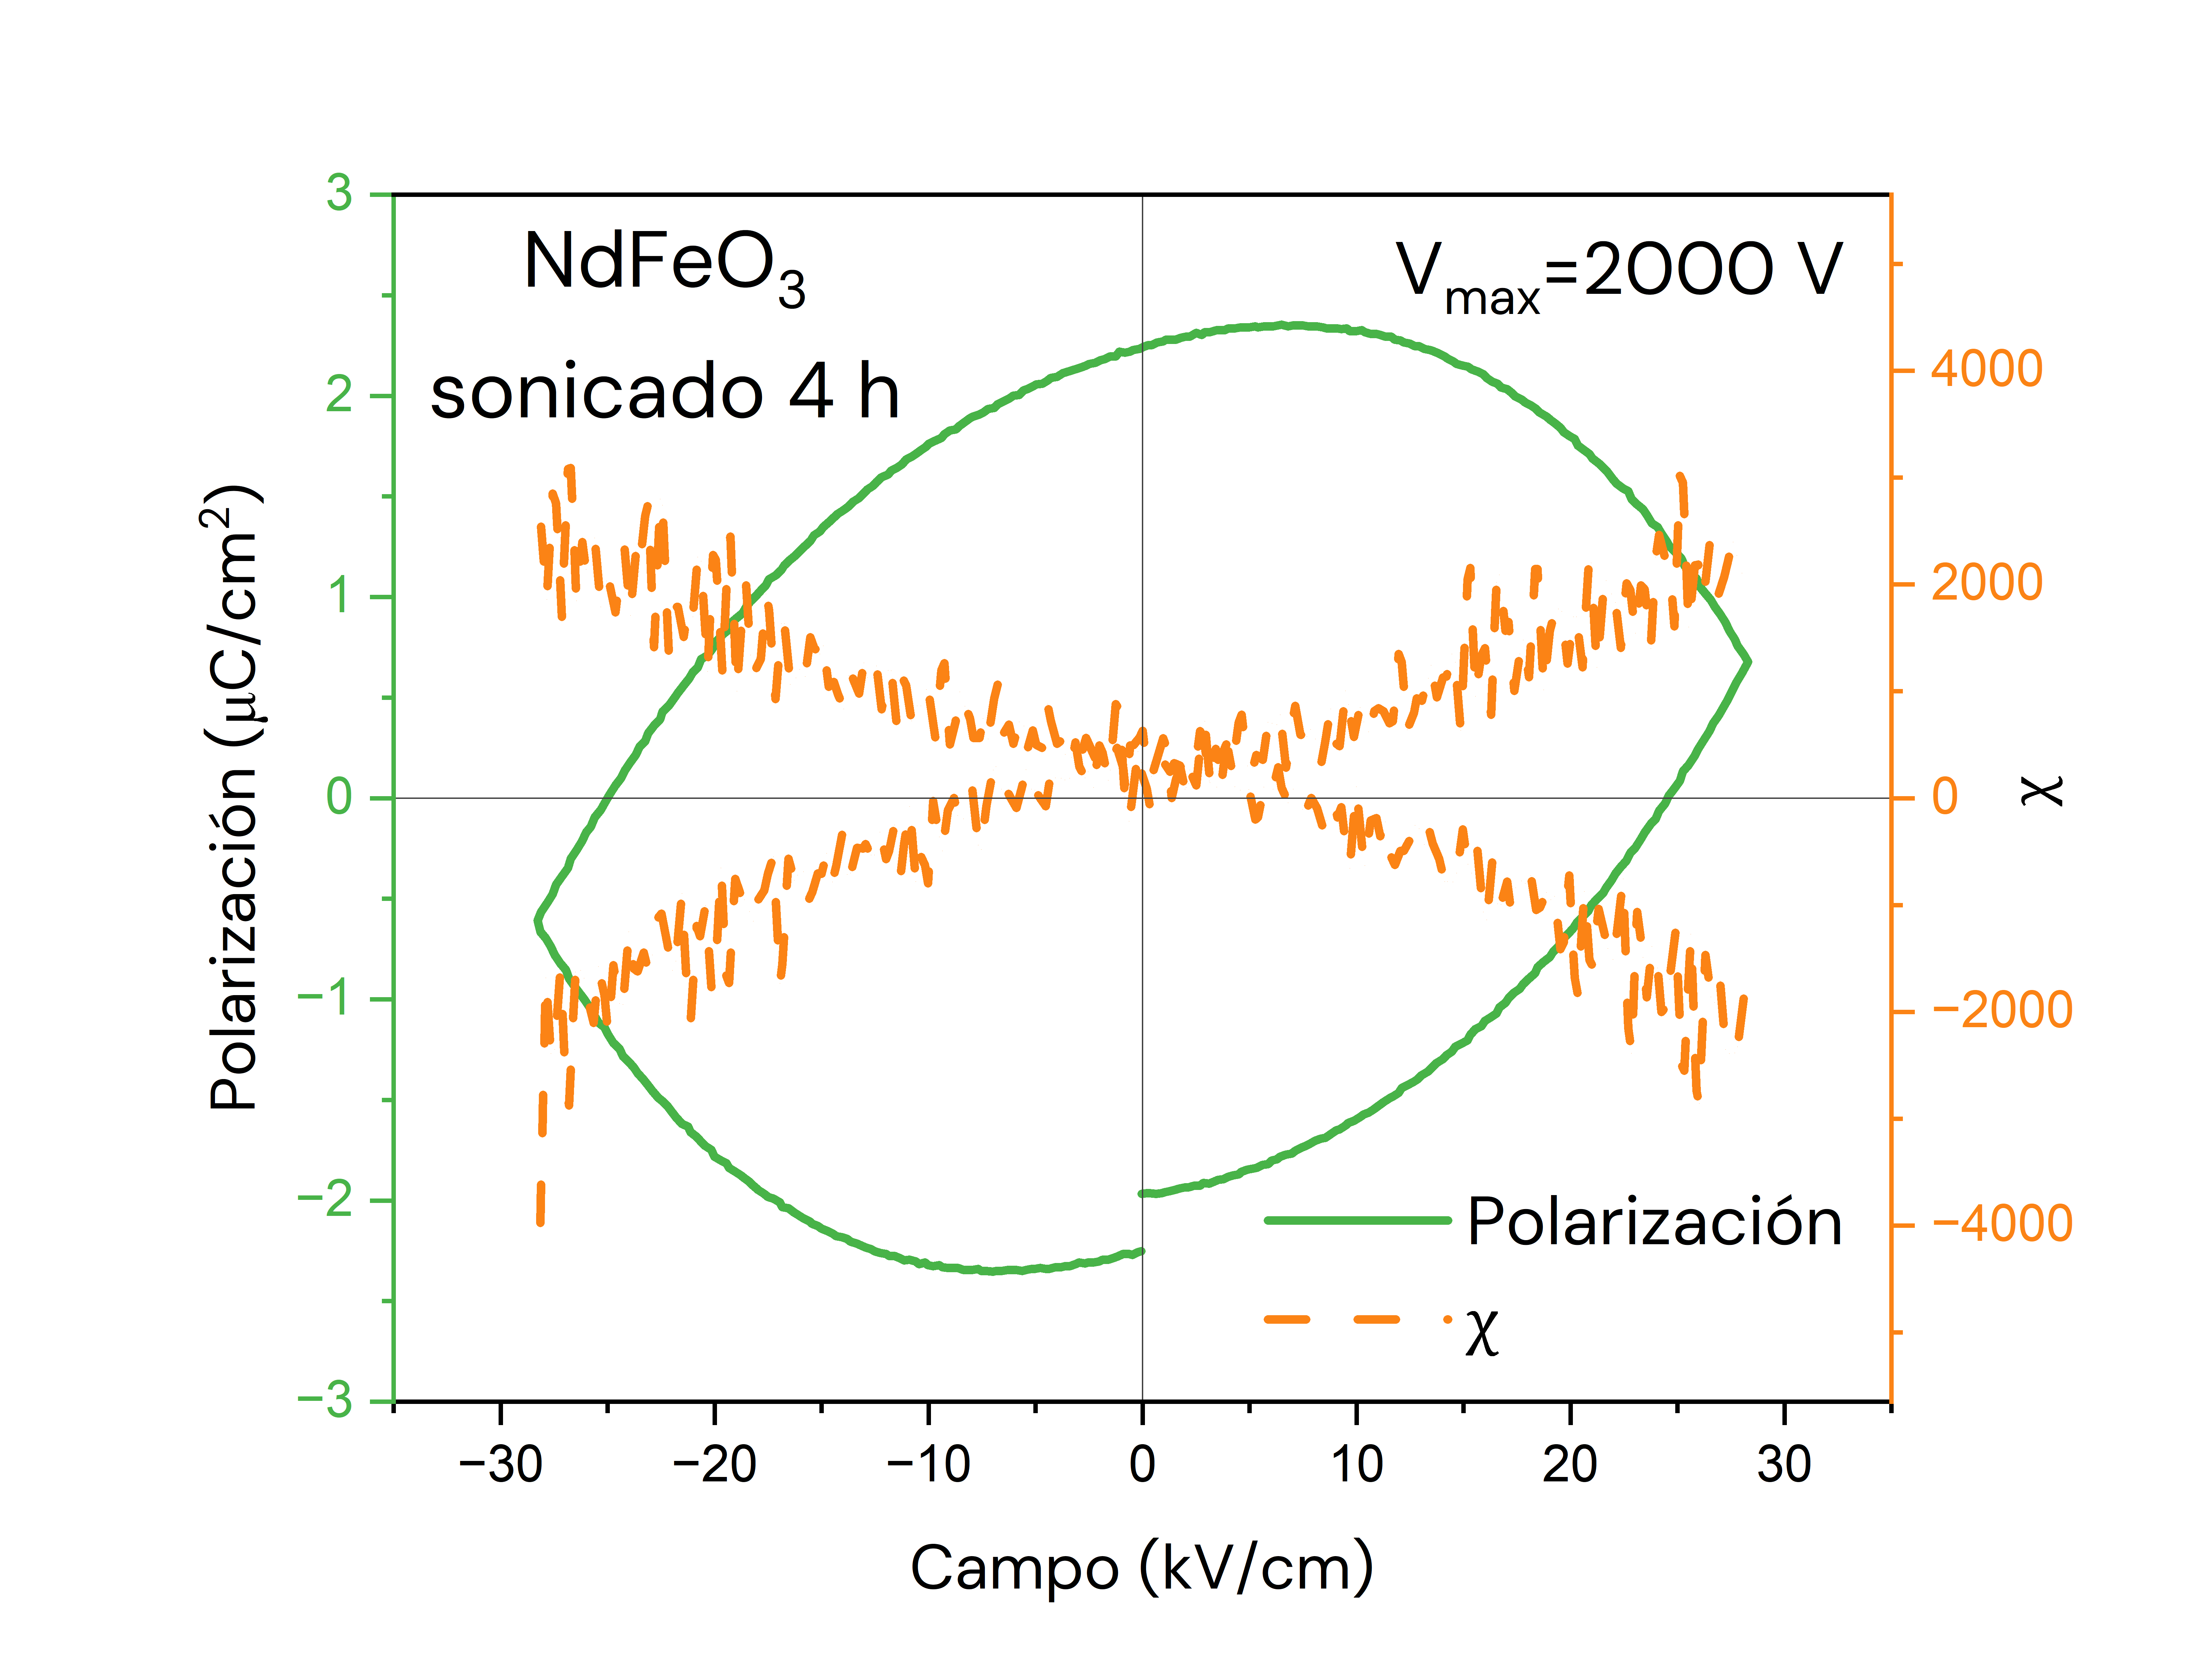
\includegraphics[width=0.45\textwidth]{fig/PENdFeO3-S2000V.png}
    \caption{Curvas $P$ contra $E$ (eje izquierdo) y $\chi$ contra $E$ (eje derecho) con $V_\text{max}=2000$ V de las muestras de \neod{}: a) sin sonicar y b) sonicada 4 h..}
    \label{fig:nd2000v}
\end{figure}
Se puede observar un comportamiento de histéresis débil sólo en las mediciones realizadas a $V_\text{max}=100$ V (figuras \ref{fig:nd100v} a) y b)), lo cual indica un comportamiento de ferroelectricidad débil. La polarización tiende a un comportamiento dependiente de la corriente similar al de un resistor al aumentar el voltaje, esto es de esperarse pues las muestras son semiconductores como se comprobó al obtener valores de \textit{band gap} típicos de este tipo de materiales en las mediciones de UV-VS, por lo cual, al aplicar un campo eléctrico más grande, los electrones de valencia pueden recibir suficiente energía para saltar a la banda de conducción.

En la tabla \ref{tabla:respolarneod} se reportan los valores obtenidos para $P_r$, $P_s$ y $E_c$ para las mediciones con $V_\text{max}=100$ V de las muestras de \neod{}.

\begin{table}[H]
    \centering
    \begin{tabular}{|c||c|c|c|}
        \hline
        Muestra & $P_s$ ($\mu$C/cm$^2$) & $P_r$ ($\mu$C/cm$^2$) & $E_c$ (kV/cm) \\
        \hline\hline
        \neod{} sin sonicar & 0.0067 $\pm$ 0.00036 & $0.0054 \pm 0.00012$ & $0.7448 \pm 0.01392$ \\
        \hline
        \neod{} sonicada & 0.0062 $\pm$ 0.00018 & $0.0044 \pm 0.00017$ & $0.6651 \pm 0.08038$ \\
        \hline
        \end{tabular} 
    \caption{Valores de $P_r$, $P_s$ y $E_c$ medidos de las muestras de \neod{} sin sonicar y sonicada 4 h.}
    \label{tabla:respolarneod}
\end{table}
\subsection{\texorpdfstring{\sama{}}{SmFeO3}}
\subsubsection{Espectroscopía UV-Vis}
De manera análoga a las muestras de \neod{}, se obtuvieron los siguientes espectros de absorción para las de \sama{} (figura \ref{fig:absorbressama}):
\begin{figure}[H]
    \centering
    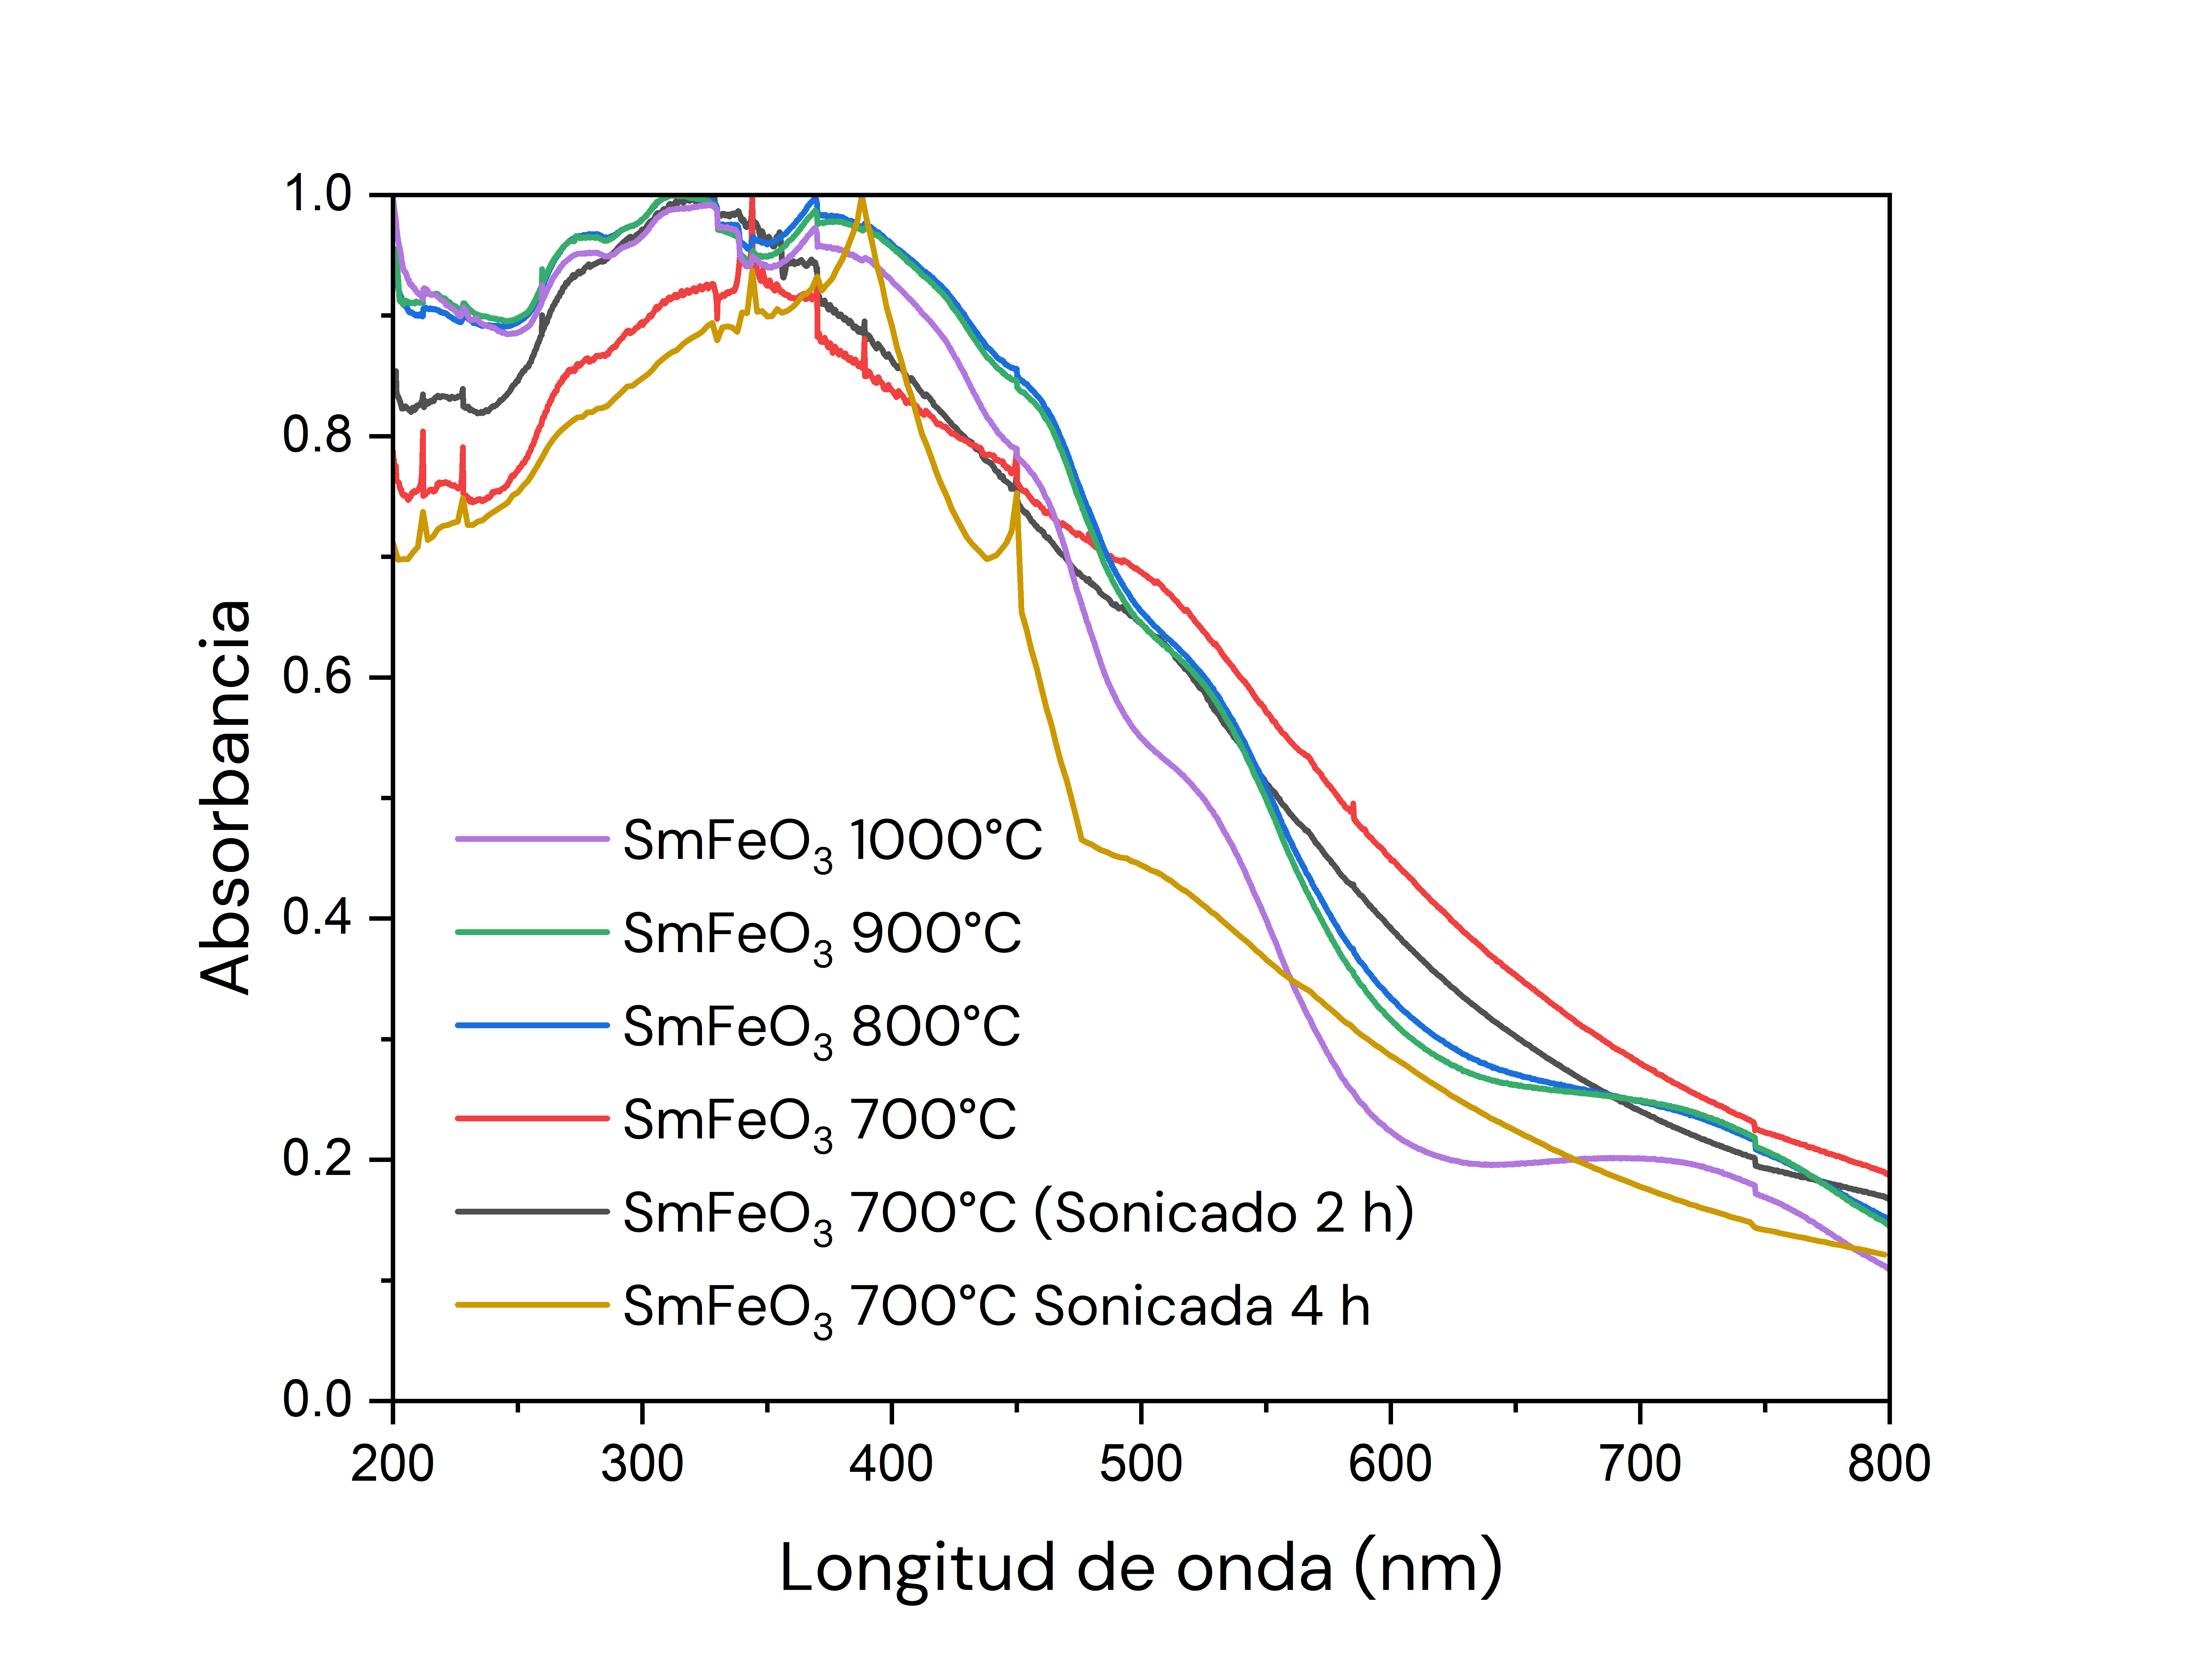
\includegraphics[width=0.7\textwidth]{fig/absorbanciasama.png}
    \caption{Gráficas de la absorbancia contra la longitud de onda para las muestras de \sama{}.}
    \label{fig:absorbressama}
\end{figure}
Aplicando el método Tauc igualmente se obtuvieron los \textit{band gaps} reportados en la tabla \ref{tabla:bandgapssama}
\begin{table}[H]
    \centering
    \begin{tabular}{|c||c|c|}
        \hline
        Muestra & Temperatura de & \textit{Band Gap} \\
        & calcinación & (eV) \\
        \hline\hline
        \multirow{6}{*}{\rotatebox[origin=c]{90}{\sama{}}} & 700\gradoC{} & 2.03$\pm$0.002 \\
        \cline{2-3}
        & 700\gradoC{}, sonicada 2 h & 2.14$\pm$0.015 \\
        \cline{2-3}
        & 700\gradoC{}, sonicada 4 h & 2.22$\pm$0.002 \\
        \cline{2-3}
        & 800\gradoC{} & 2.20$\pm$0.001 \\
        \cline{2-3}
        & 900\gradoC{} & 2.21$\pm$0.001 \\
        \cline{2-3}
        & 1000\gradoC{} & 2.30$\pm$0.001 \\
        \hline
    \end{tabular} 
    \caption{\textit{Band gaps} de las distintas muestras según su temperatura de calcinación.}
    \label{tabla:bandgapssama}
\end{table}
\begin{figure}[H]
    \centering
    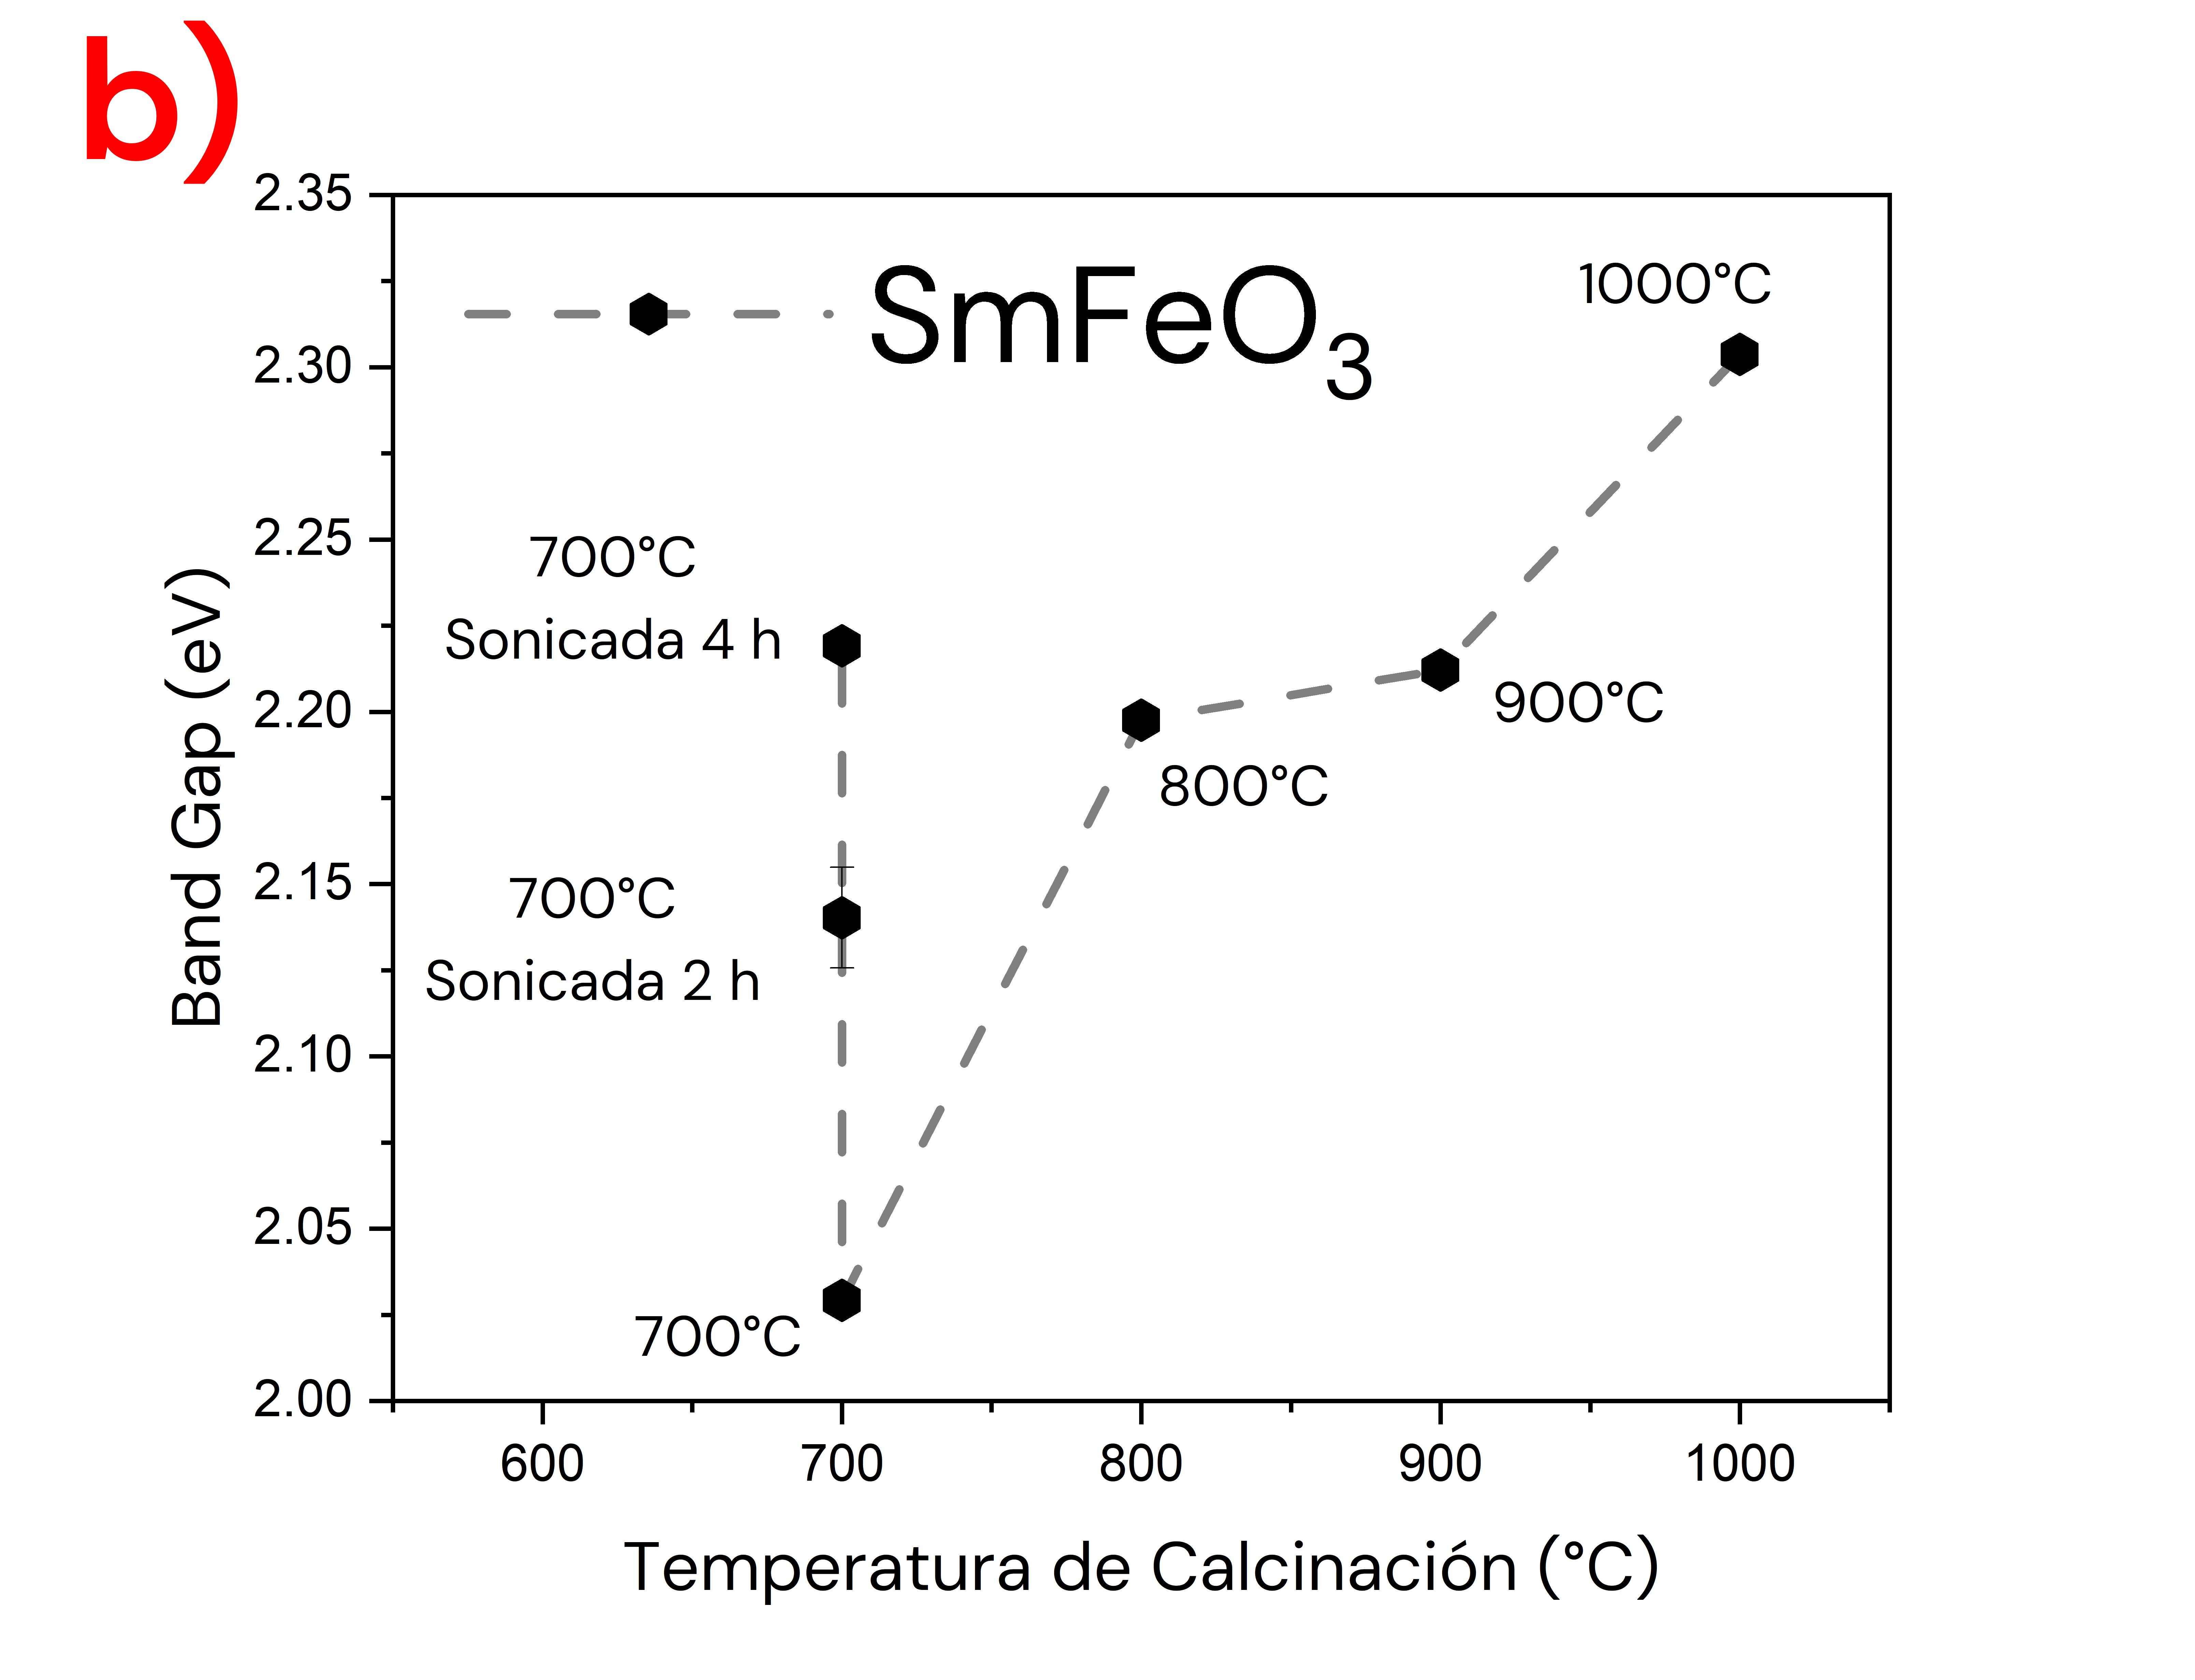
\includegraphics[width=0.7\textwidth]{fig/BGSmFeO3.png}
    \caption{Gráfica del \textit{band gap} de cada muestra de \sama{} según su temperatura de calcinación.}
    \label{fig:bandgapvT}
\end{figure}
En este caso también se observa que el \textit{band gap} aumenta con la temperatura y el tiempo de sonicación, ocurriendo de la misma forma un mínimo en la muestra calcinada a menor temperatura y sin sonicar.
\subsubsection{Magnetometría SQUID}
Se obtuvieron las siguientes curvas de $M$ vs $H$, $M$ vs $T$ y $\chi^{-1}$ vs $T$ para las muestras de \sama{}  calcinadas a 700\gradoC{} y 900\gradoC{}:
\begin{figure}[H]
    \centering
    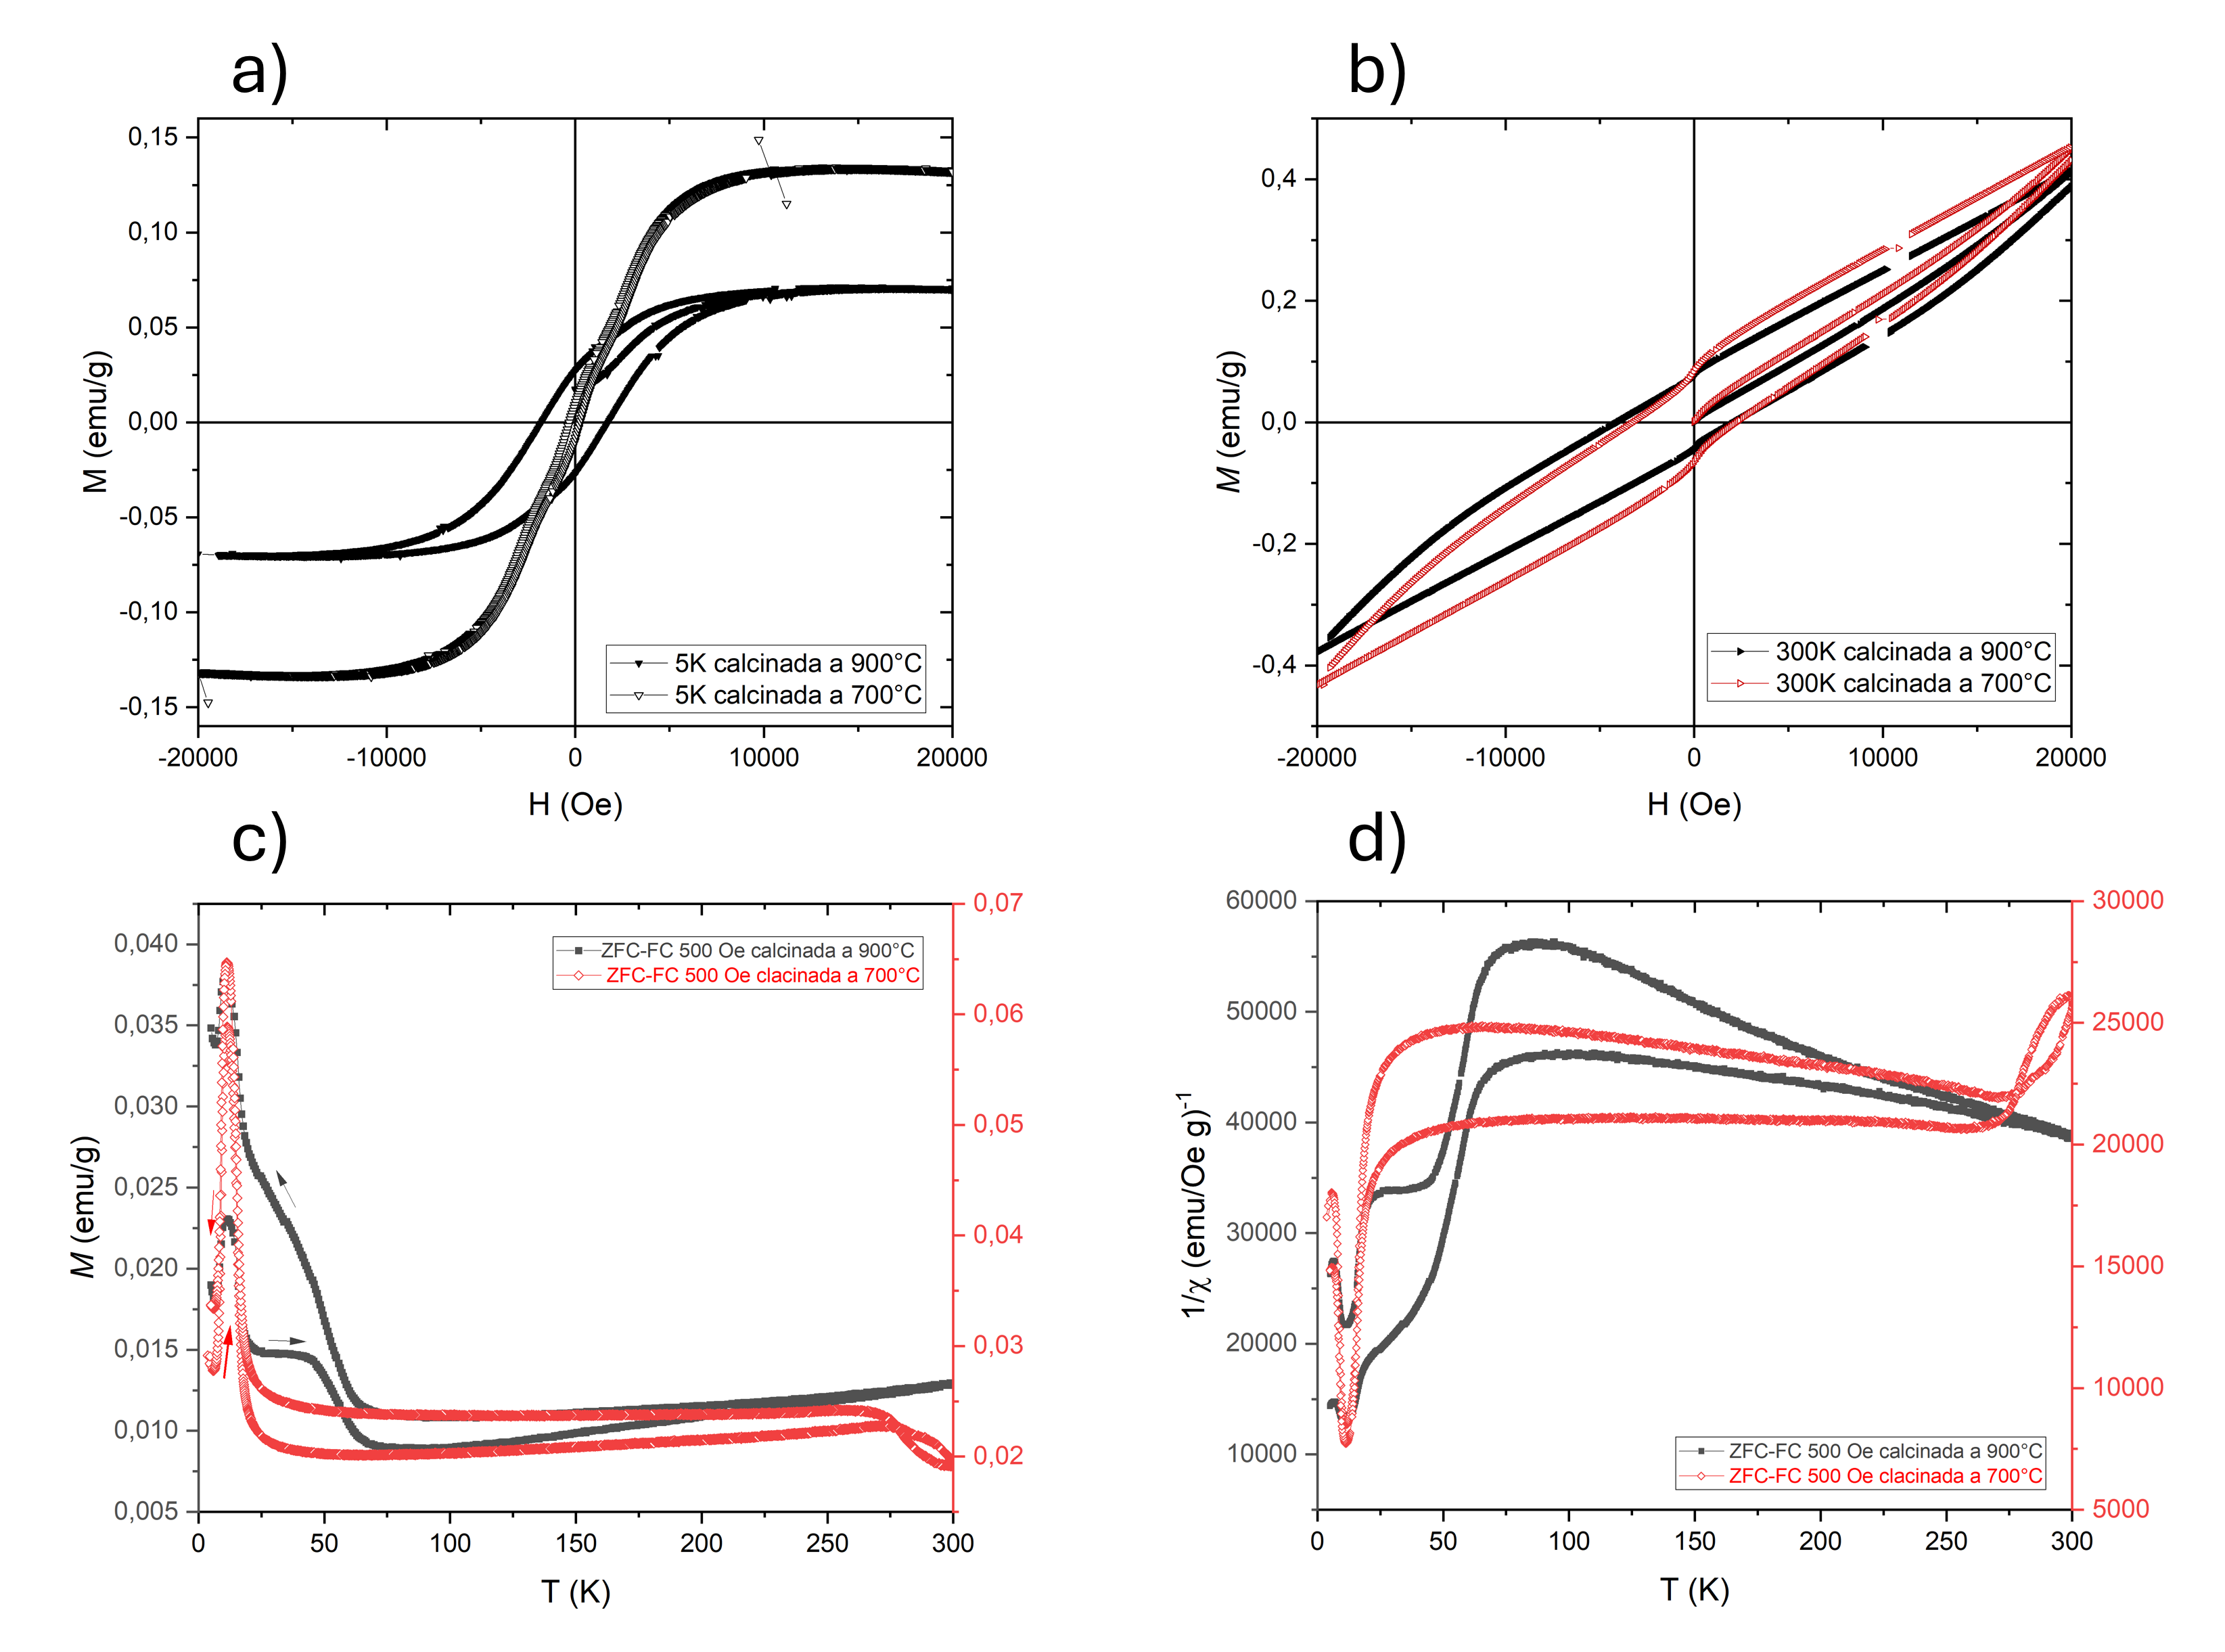
\includegraphics[width=0.9\textwidth]{fig/Magnetometria_SmFeO3_calc.png}
    \caption{Magnetometría de las muestras \sama{} calcinadas a 700\gradoC{} y a 900\gradoC{}: a) Curvas $M$ vs $H$ a 5 K para las muestras calcinadas a 700\gradoC{}  (triángulos vacíos negros) y a 900\gradoC{} (triángulos llenos negros), b) Curvas $M$ vs $H$ a 300 K para las muestras calcinadas a 700\gradoC{}  (triángulos vacíos rojos) y a 900\gradoC{} (triángulos llenos negros), c)   $M$ vs $T$ FC-ZFC a 500 Oe para la muestra calcinada a 700\gradoC{} (diamantes vacíos rojos) y a 900\gradoC{} (cuadrados llenos grises)d) $\chi^{-1}$ vs $T$ a 500 Oe para la muestra calcinada a 700\gradoC{} (diamantes vacíos rojos) y a 900\gradoC{} (cuadrados llenos grises).}
    \label{fig:mvhSm}
\end{figure}

A diferencia del \neod{}, la muestra de \sama{} calcinada a 900\gradoC{} muestra un comportamiento ferromagnético a 5 K (triángulos llenos de la figura \ref{fig:mvhSm} a)), sin embargo, la muestra calcinada a 700\gradoC{} muestra una magnetización de saturación mayor pero un campo coercitivo muy reducido y un ligero efecto de escalón a $\sim$ 2300 Oe característico del acoplamiento antiferromagnético con una red ferromagnética. Ambas muestras presentan un comportamiento de ferromagnético débil a 300K (figura \ref{fig:mvhSm} b)) independientemente de la temperatura de calcinación.

En la figura \ref{fig:mvhSm} c) se muestran las curvas $M$ vs $T$ enfriadas sin campo (ZFC) y con campo (FC) con un campo externo de 500 Oe para la muestra calcinada a 700\gradoC{} (curva roja) y a 900\gradoC{} (curva gris).  El repentino aumento de la pendiente por debajo de 25 K indica que los espines \ce{Nd^{3+}} se ordenan en el campo de intercambio de los espines \ce{Fe^{3+}}. Sin embargo al continuar enfriando la muestra, se observa un máximo en $\sim$ 10K por debajo del cual $M$ es decreciente. Esto ocurre tanto en las curvas FC como ZFC, lo cual indica una alineación de espines predominantemente antiparalela.

A medida que baja la temperatura y los iones de tierras raras se polarizan cada vez más, su anisotropía efectiva aumenta y la ortoferrita puede sufrir una transición de reorientación de espín (SR) en la que los espines de Fe se reorientan, pasando de estar paralelos (aparte de la pequeña inclinación producto de la interacción de Dzyaloshinskii-Moriya) al eje $c$ por debajo de $T_{SR2}$ a estar paralelos al eje $a$ por encima de $T_{SR1}$.

Según la simetría cristalina, hay tres configuraciones de espín de Fe permitidas en RFeO3, etiquetadas como $\Gamma_{4} (G_{x}, A_{y}, F_{z})$, $\Gamma_{2} (F_{x}, C_{y}, G_{z})$ y $\Gamma_{1} (A_{x}, G_{y}, C_{z})$. Las letras $G$ (vector antiferromagnético), $C$ (vector antiferromagnético débil), $A$ (vector antiferromagnético débil) y $F$ (vector ferromagnético) son notaciones de Bertaut que se introdujeron en la sección del estado del arte \cite{Bertaut1963}. La configuración $\Gamma_{1}$ no presenta momento magnético neto, mientras que $\Gamma_{2}$ y $\Gamma_{4}$ muestran un pequeño momento  ferromagnético en las direcciones $x$ y $z$, respectivamente. En la mayoría de las ortoferritas de tierras raras, con la reorientación del espín, las configuraciones del espín cambian de la fase de alta temperatura $\Gamma_{4}$ a la fase de baja temperatura $\Gamma_{2}$.

La figura \ref{fig:mvhNd} (d) muestra las curvas de susceptibilidad magnética recíproca $\chi^{-1}$ en función de la temperatura $T$ de ambas muestras, a partir de las cuales podemos obtener la información sobre la reorientación del espín.  Los máximos y mínimos que aparecen en esta figura indican la presencia de estas reorientaciones de espín en ambas muestras las cuales ocurren en el rango de temperaturas bajas $T_{SR2}-T_{SR1} \sim 6-15 K $, sin embargo para la muestra calcinada a 900\gradoC{} parece haber una fase adicional entre $25-50$ K.

En la figura \ref{fig:M_Sm_sonic} a) se observa que la muestra calcinada a 700\gradoC{} y sometida a un proceso de sonicación presenta las propiedades de un ferromagnético débil cuya curva de histéresis se vuelve mucho menos pronunciada y tiende a un comportamiento más lineal a 300 K. A temperatura ambiente no se observan diferencias significativas respecto a la muestra sin sonicar (figura \ref{fig:M_Sm_sonic} b)).

Por otro lado, en la figura \ref{fig:M_Sm_sonic} c) y d) se puede observar que la muestra sonicada tiene un comportamiento más parecido al que se observó en las muestras de \neod calcinadas a 600\gradoC donde el repentino aumento de la pendiente por debajo de 25 K indica que los espines \ce{Sm^{3+}} se ordenan en el campo de intercambio de los espines \ce{Fe^{3+}}, lo que se refleja en el aumento inicial $M(T)$. Sin embargo, se observa la presencia un máximo y un mínimo local (curva morada de la figura \ref{fig:M_Sm_sonic} d)) que indica la ocurrencia de reorientación de espines en el mismo rango de temperaturas $T_{SR2}-T_{SR1} \sim 8-17$ K aunque mucho menos pronunciado que en la muestra sin sonicar.Para temperaturas por debajo de ese mínimo local a $\sim$ 8 K, $M(T)$ continúa aumentando tanto para la curva enfriada con campo (FC) como para aquella enfriada sin campo (ZFC).

\begin{figure}[H]
    \centering
    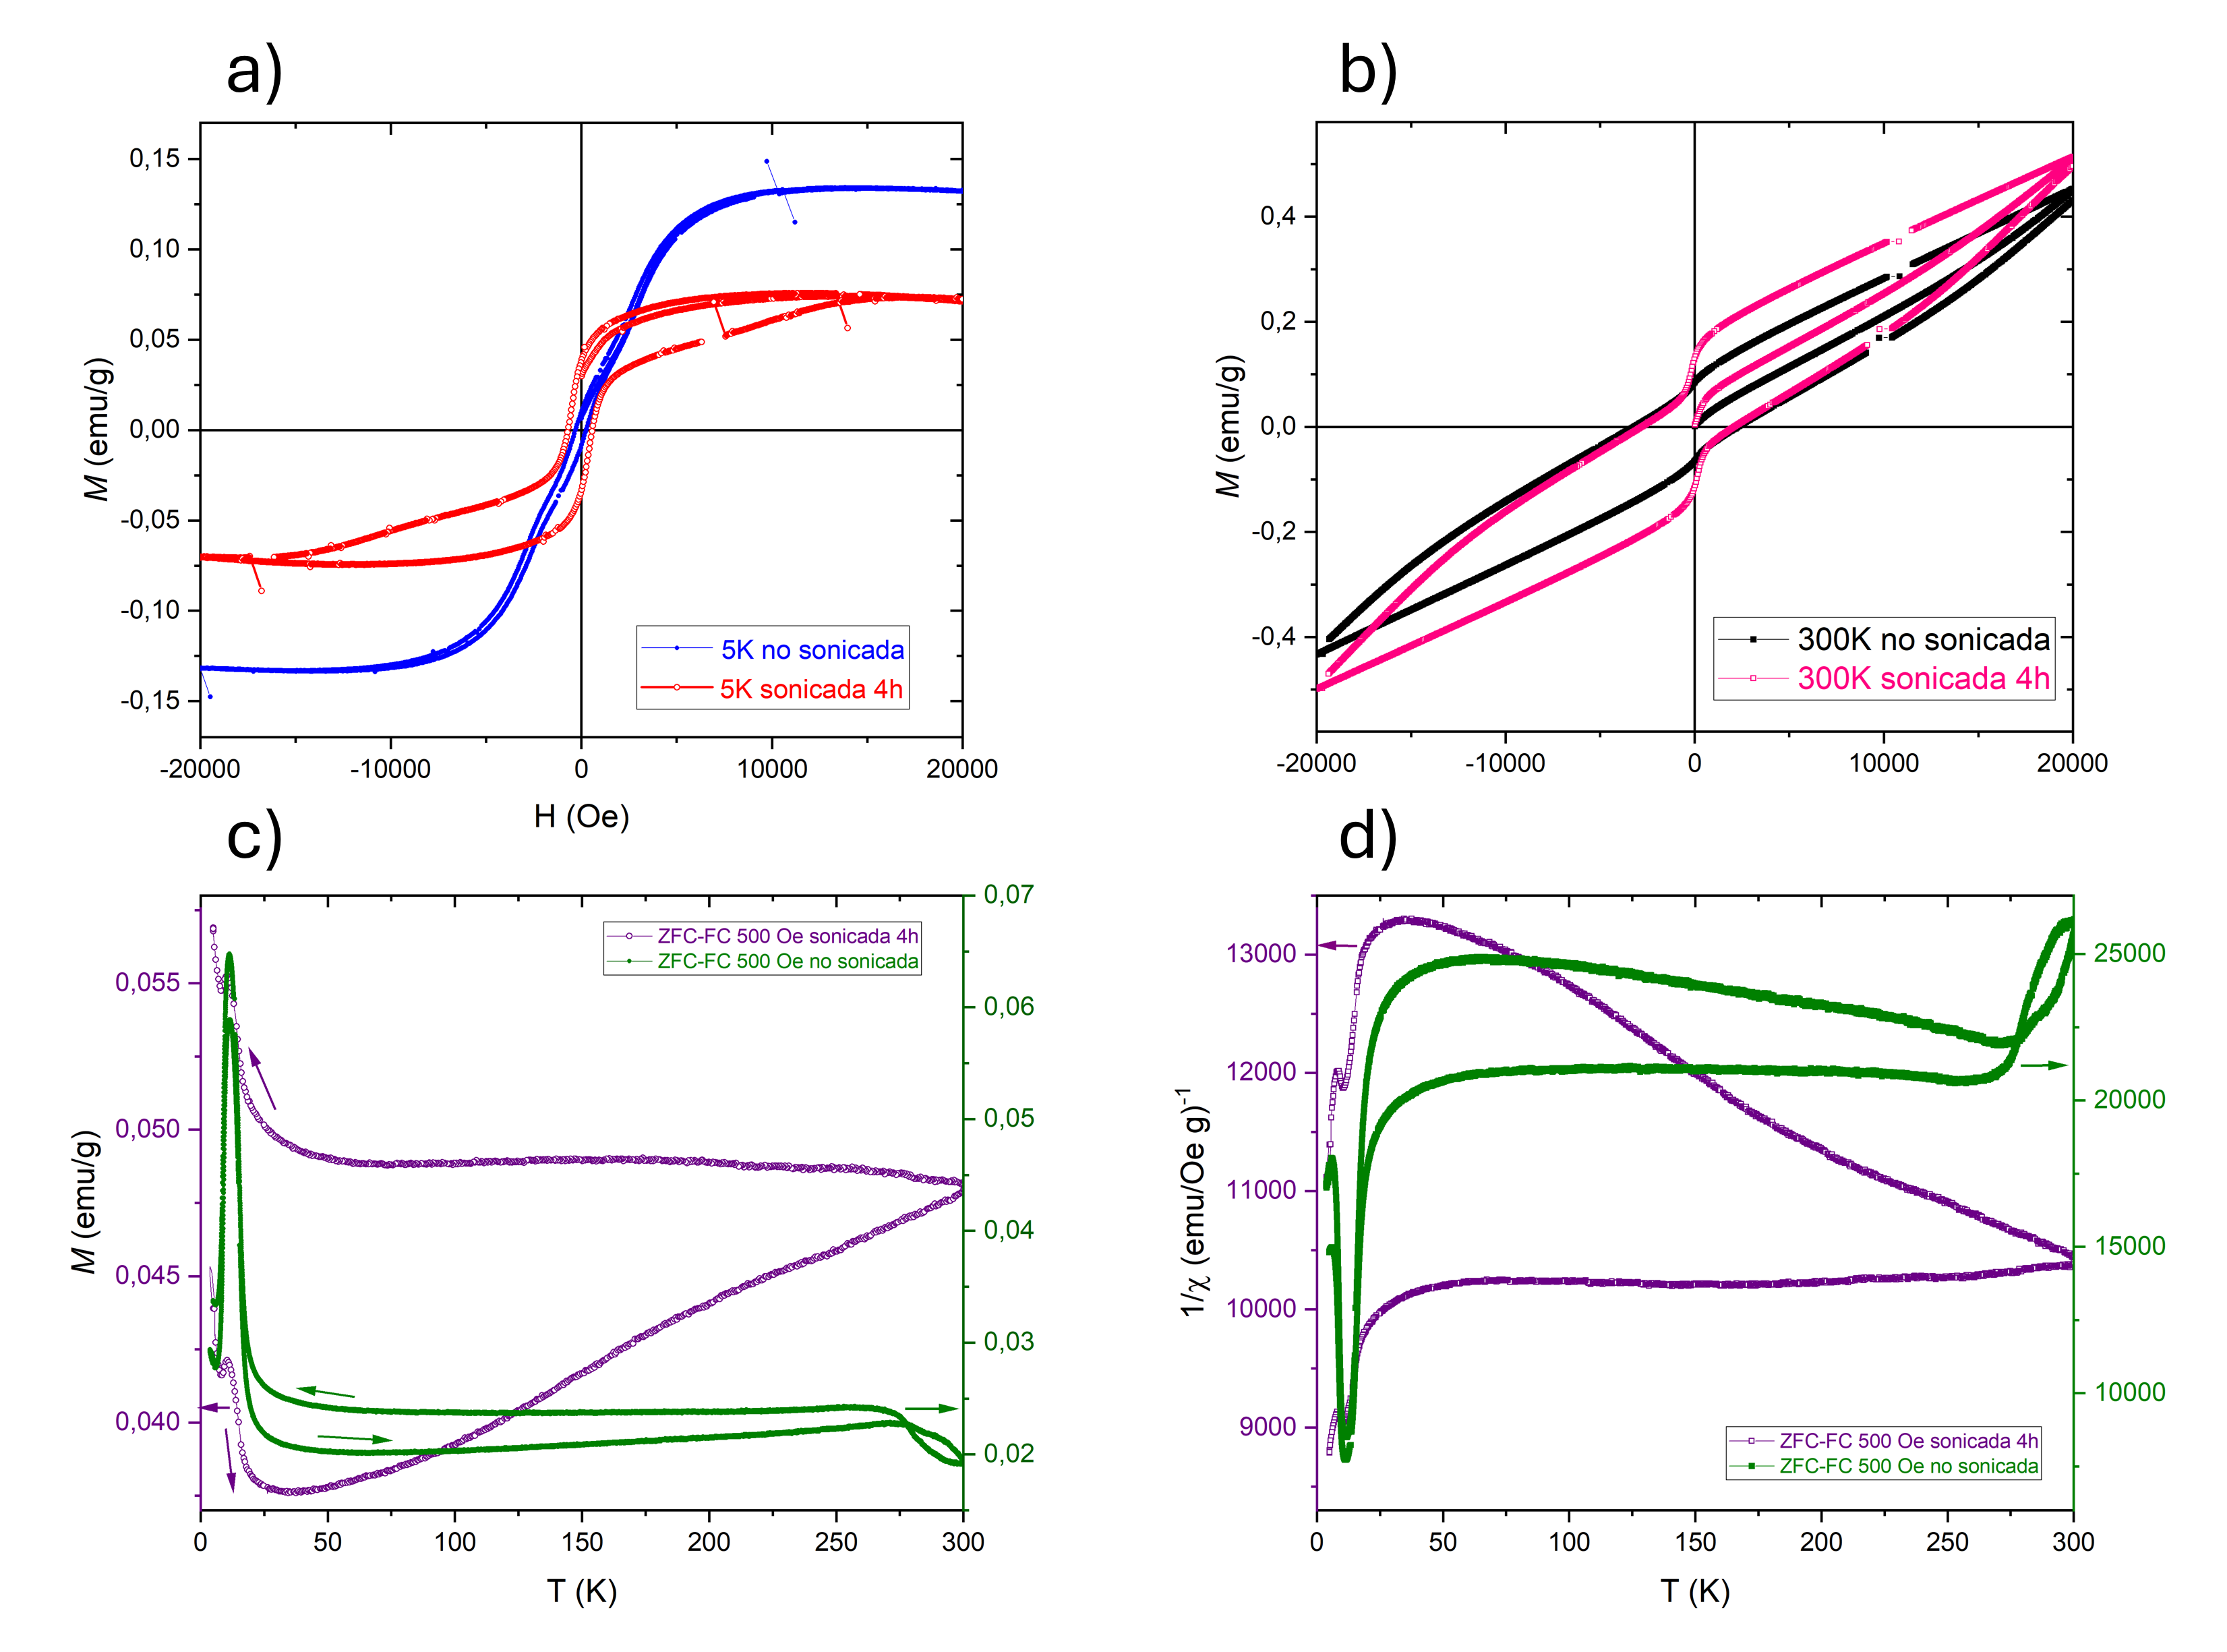
\includegraphics[width=0.9\textwidth]{fig/Magnetometria_SmFeO3_sonic.png}
    \caption{Magnetometría de las muestras de \sama{} calcinadas a 700\gradoC{} sin sonicar y sonicada durante 4h: a) Curvas $M$ vs $H$ a 5K para las muestras sin sonicar  (puntos llenos azules) y sonicadas (puntos rojos vacíos), b) Curvas $M$ vs $H$ a 300K sin sonicar  (cuadrados llenos negros) y sonicadas  (cuadrados vacíos rosas),  c) $M$ vs $T$ FC-ZFC a 500 Oe para la muestra sin sonicar (círculos llenos verdes) y sonicada (círculos vacíos morados) d) $\chi^{-1}$ vs $T$ a 500 Oe  para la muestra sin sonicar  (círculos llenos verdes) y sonicada (círculos vacíos morados)}
    \label{fig:M_Sm_sonic}
\end{figure}

En la siguiente tabla se reportan los valores obtenidos para $M_r$, $M_s$ y $H_c$ en todas las muestras de \sama.

\begin{table}[H]
	\centering
	\begin{tabular}{|c||c|c|c|}
		\hline 
		Muestra & $M_s$ (emu/g) & $M_r$ (emu/g) & $H_c$ (Oe) \\
		\hline
		\hline
		\multicolumn{4}{|c|}{$T=5$ K} \\
		\hline 
		\sama{} (700\gradoC{}) sin sonicar & 0.13$\pm$0.002 & 0.01$\pm$0.004 & 252.014$\pm$5.531 \\
		\hline
		\sama{} (700\gradoC{}) sonicada 4 h & 0.04$\pm$0.001 & 0.08$\pm$0.002 & 591.54$\pm$20.834 \\
		\hline
        \sama{} (900\gradoC{}) & 0.06$\pm$0.002 & 0.02$\pm$0.001 & 1823.26$\pm$72.416 \\
		\hline
		\multicolumn{4}{|c|}{$T=300$ K} \\
		\hline
		\sama{} (700\gradoC{}) sin sonicar & 0.06$\pm$0.001 & 0.07$\pm$0.001 & 2206.76$\pm$41.575 \\
		\hline
		\sama{} (700\gradoC{}) sonicada 4 h & 0.17$\pm$0.002 & 0.12$\pm$0.001 & 1561.36$\pm$20.612 \\
		\hline
		\sama{} (900\gradoC{}) & 0.08$\pm$0.001 & 0.07$\pm$0.003 & 4011.14$\pm$148.208 \\
		\hline
	\end{tabular} 
	\caption{Valores de $M_s$, $M_r$ y $H_c$ obtenidos para las muestras de \sama{}.}
	\label{tabla:resmvhsama}
\end{table}
\subsubsection{Curvas de polarización}
En las figuras \ref{fig:sm100v} y \ref{fig:sm2000v} se reportan las curvas $P$ vs $E$ de las muestras de \sama{} sinterizadas con un voltaje aplicado máximo de $V_{max}=$ 100 y 2000 V respectivamente.
\begin{figure}[H]
    \centering
    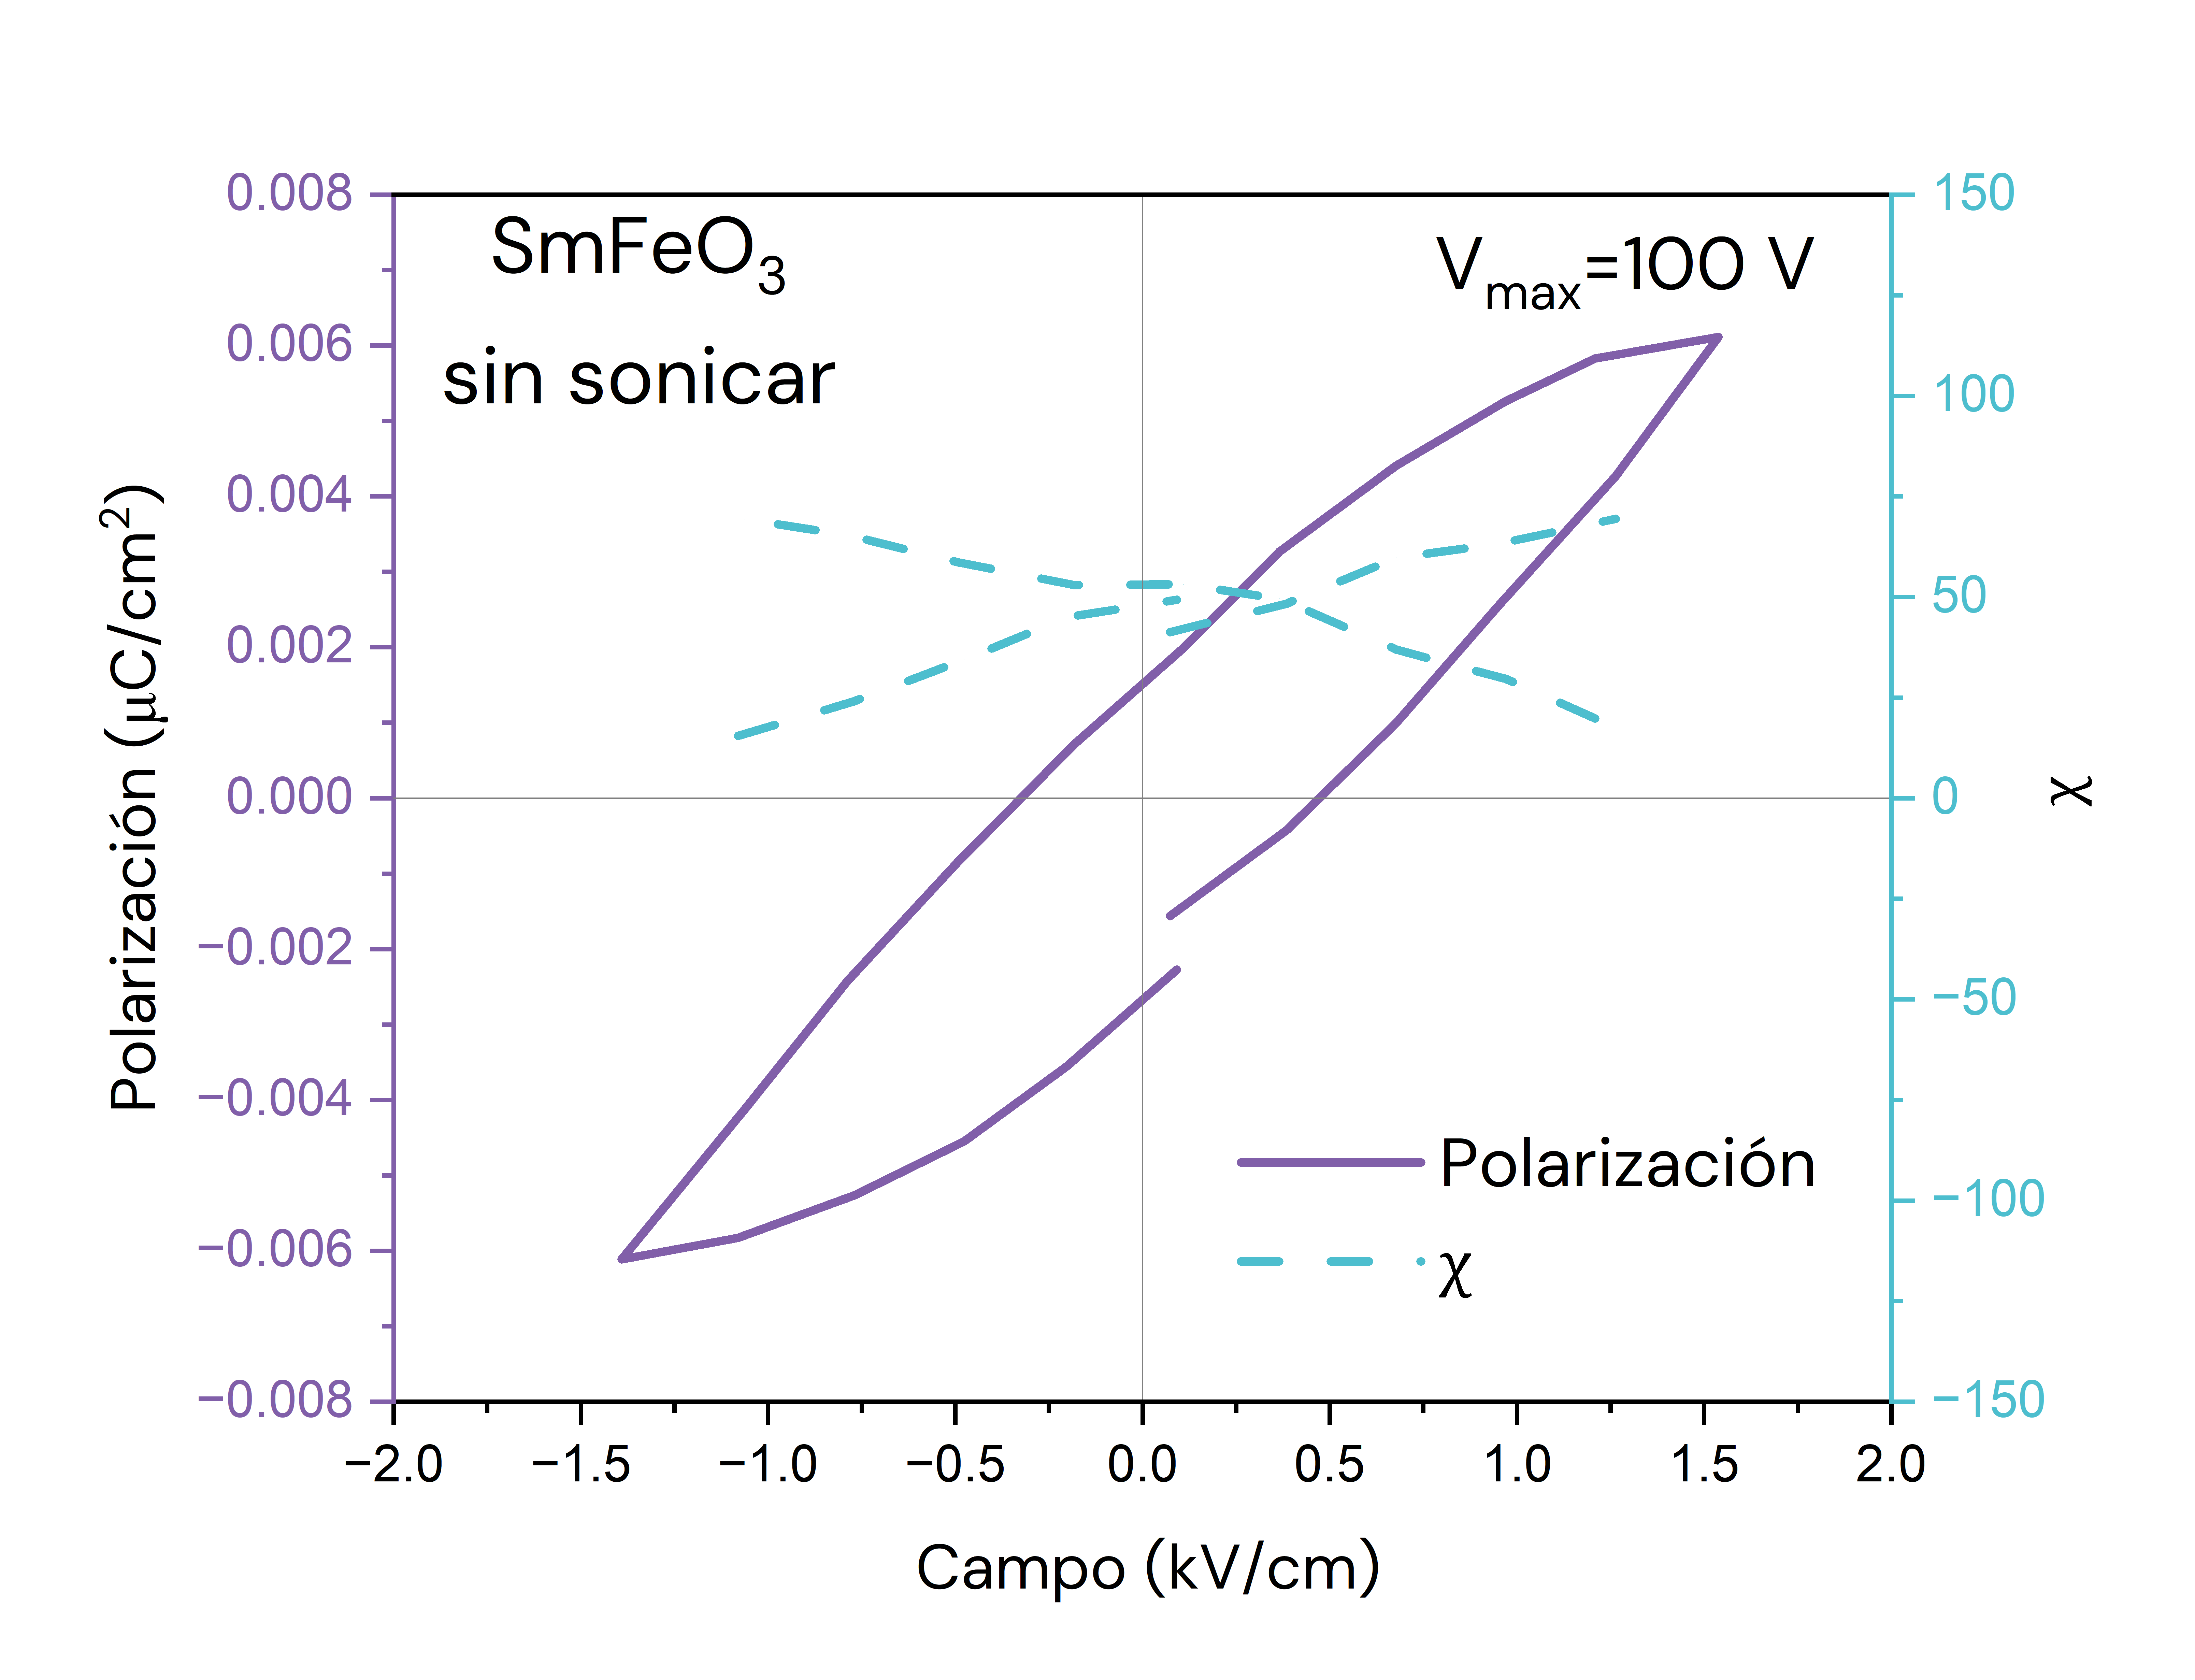
\includegraphics[width=0.45\textwidth]{fig/PESmFeO3100V.png}
    \quad
    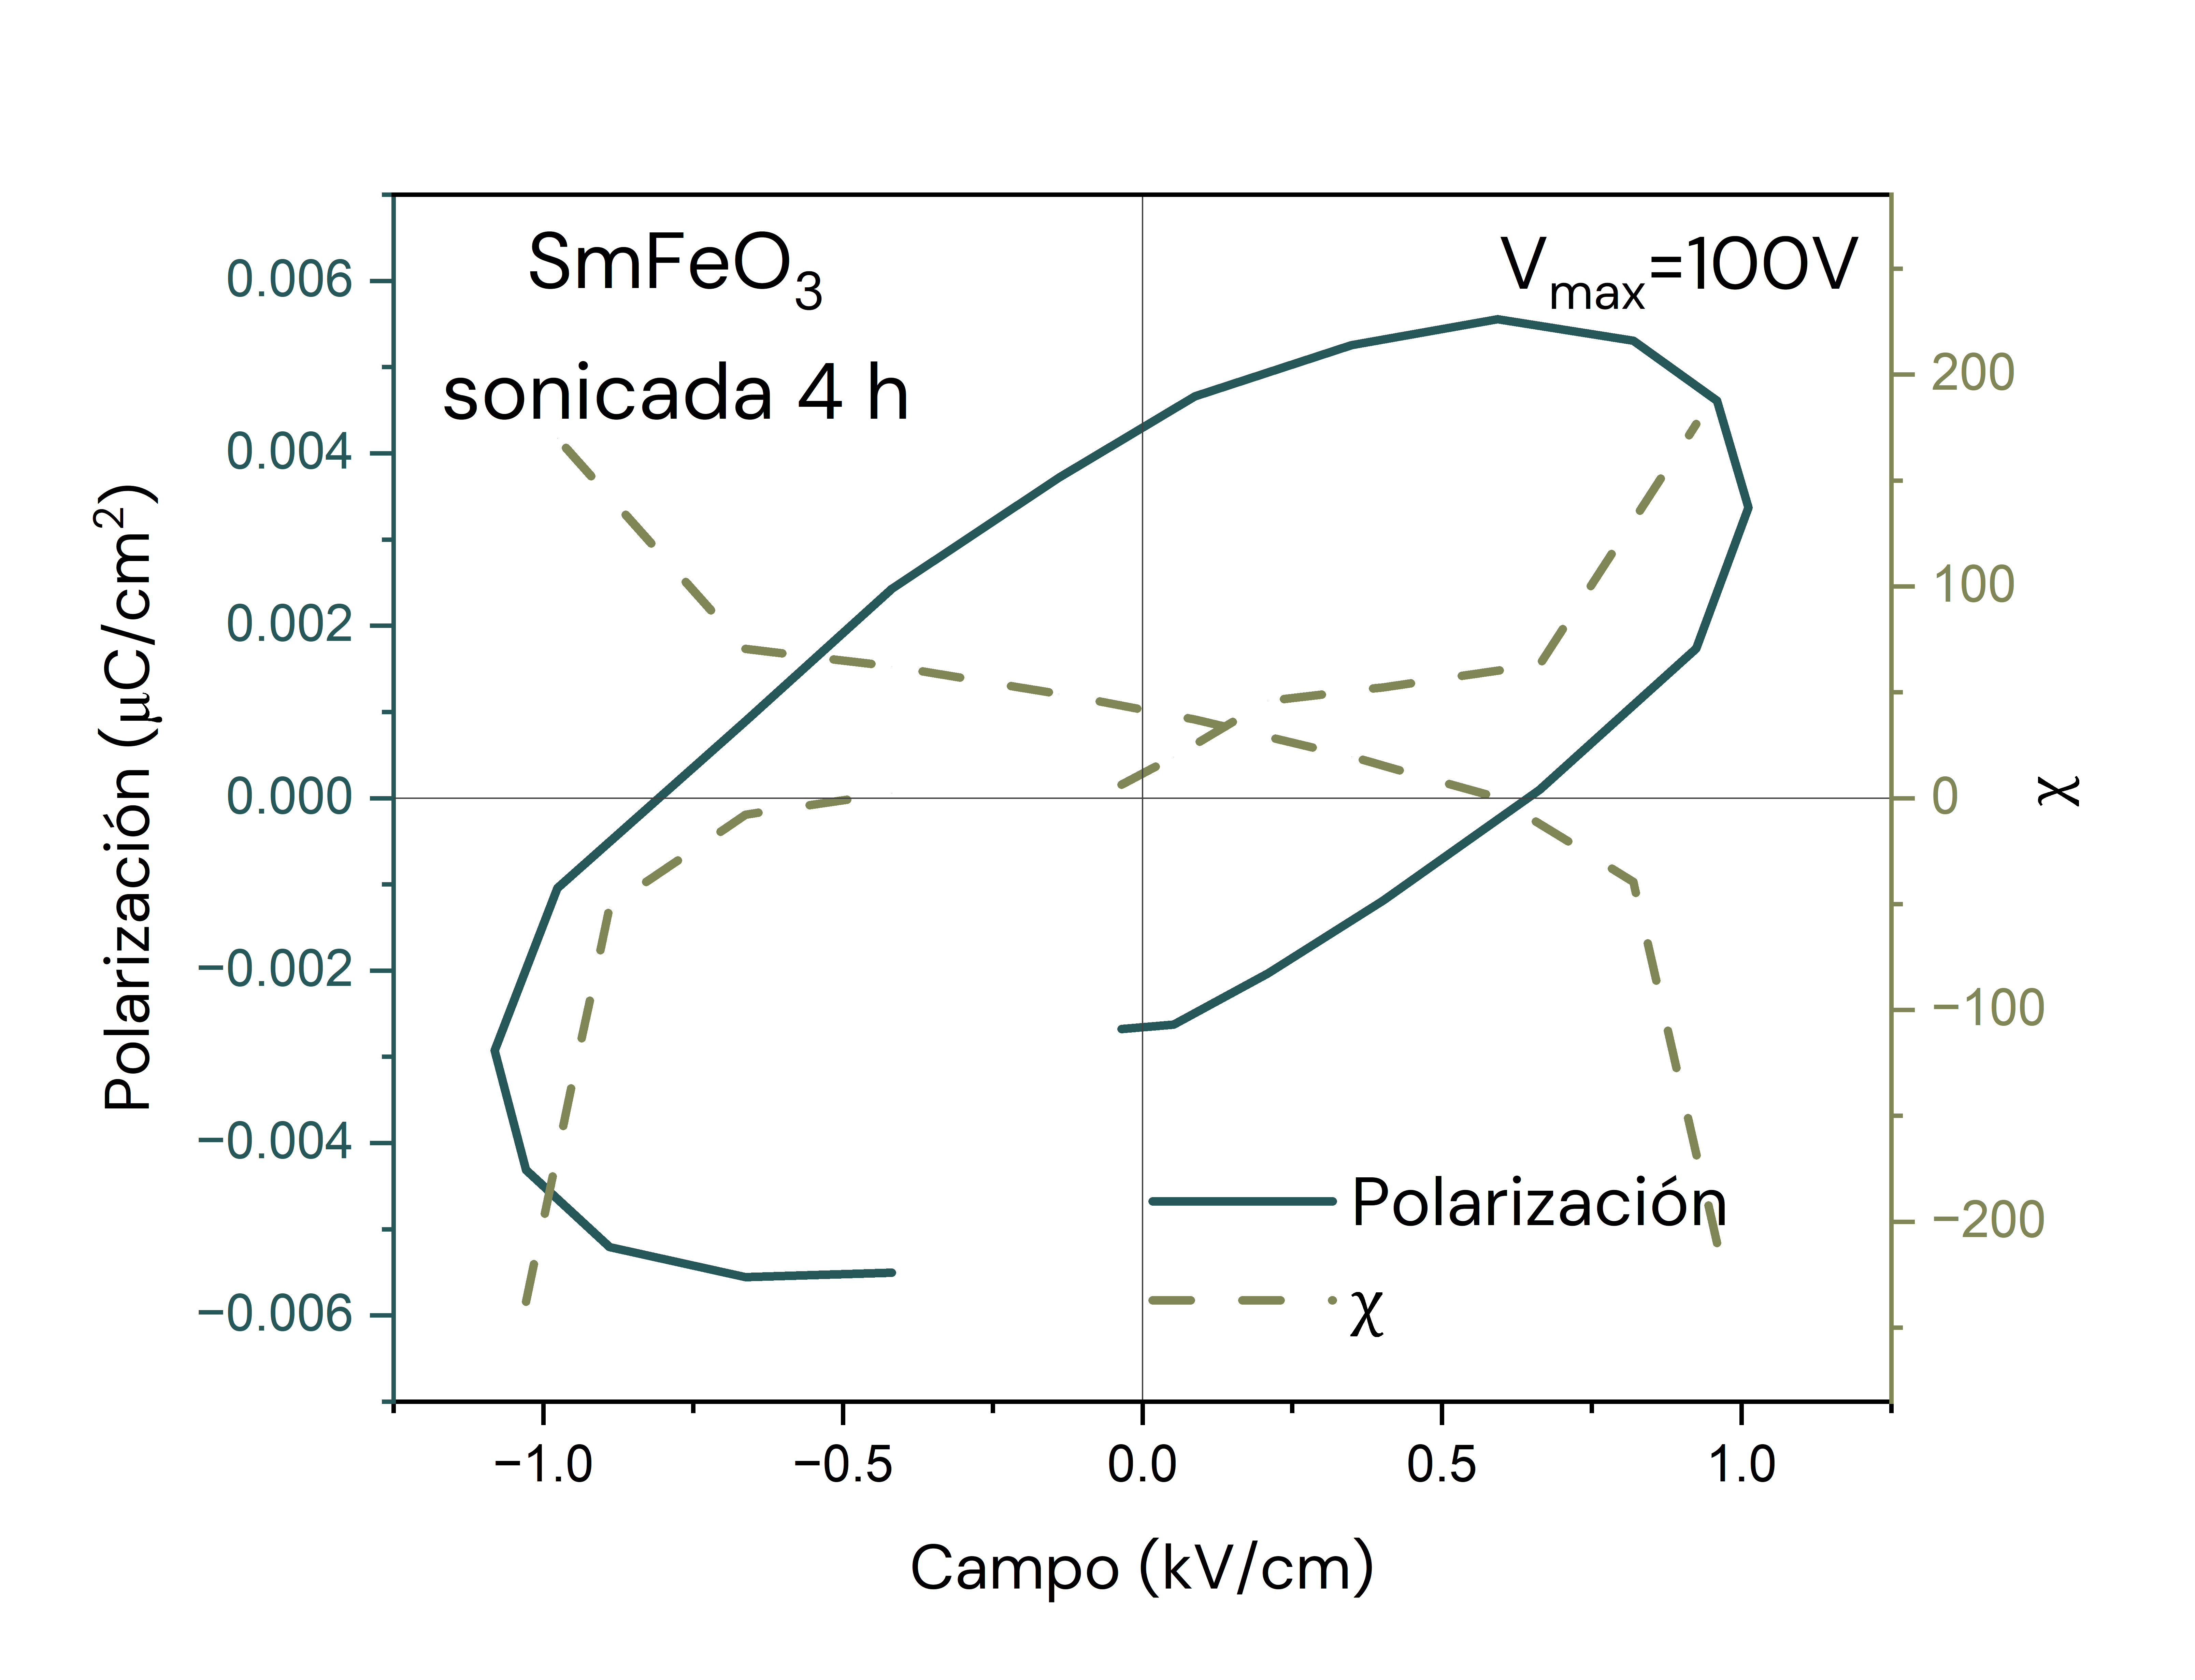
\includegraphics[width=0.45\textwidth]{fig/PESmFeO3-S100V.png}
    \caption{Curvas $P$ contra $E$ (eje izquierdo) y $\chi$ contra $E$ (eje derecho) con $V_\text{max}=100$ V de las muestras de \sama{}: a) sin sonicar y b) sonicada 4 h.}
    \label{fig:sm100v}
\end{figure}
\begin{figure}[H]
    \centering
    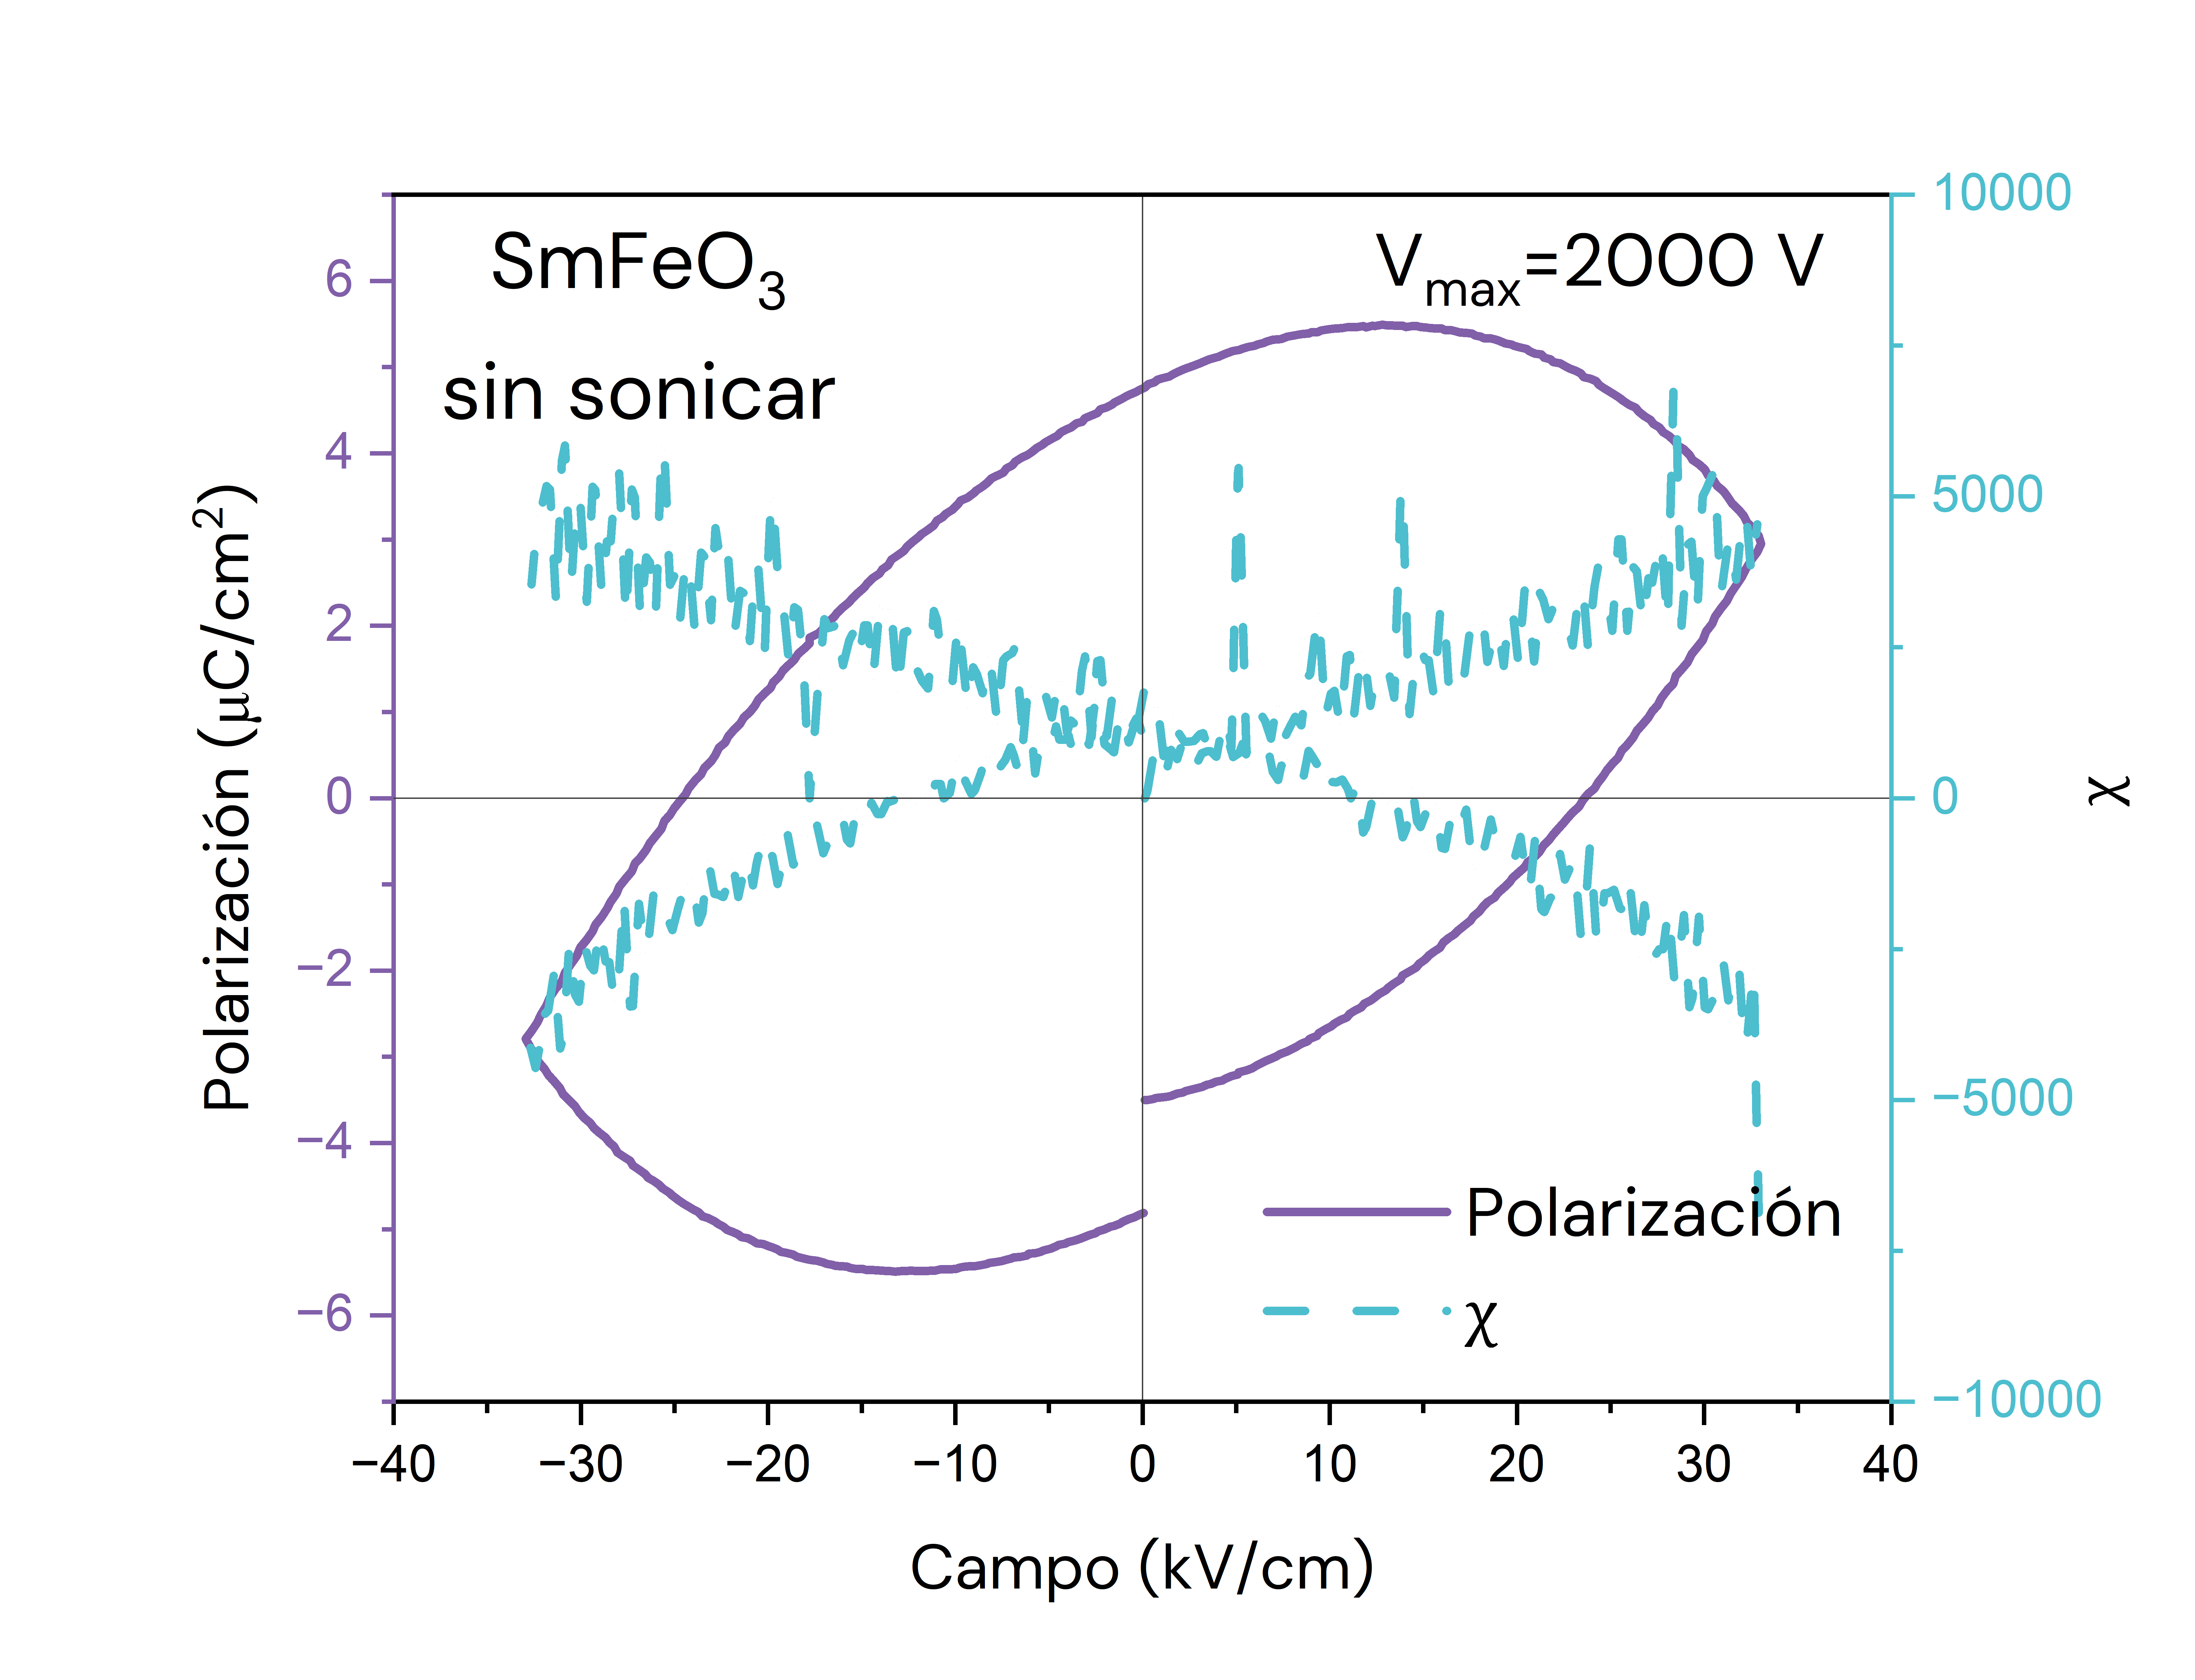
\includegraphics[width=0.45\textwidth]{fig/PESmFeO32000V.png}
    \quad
    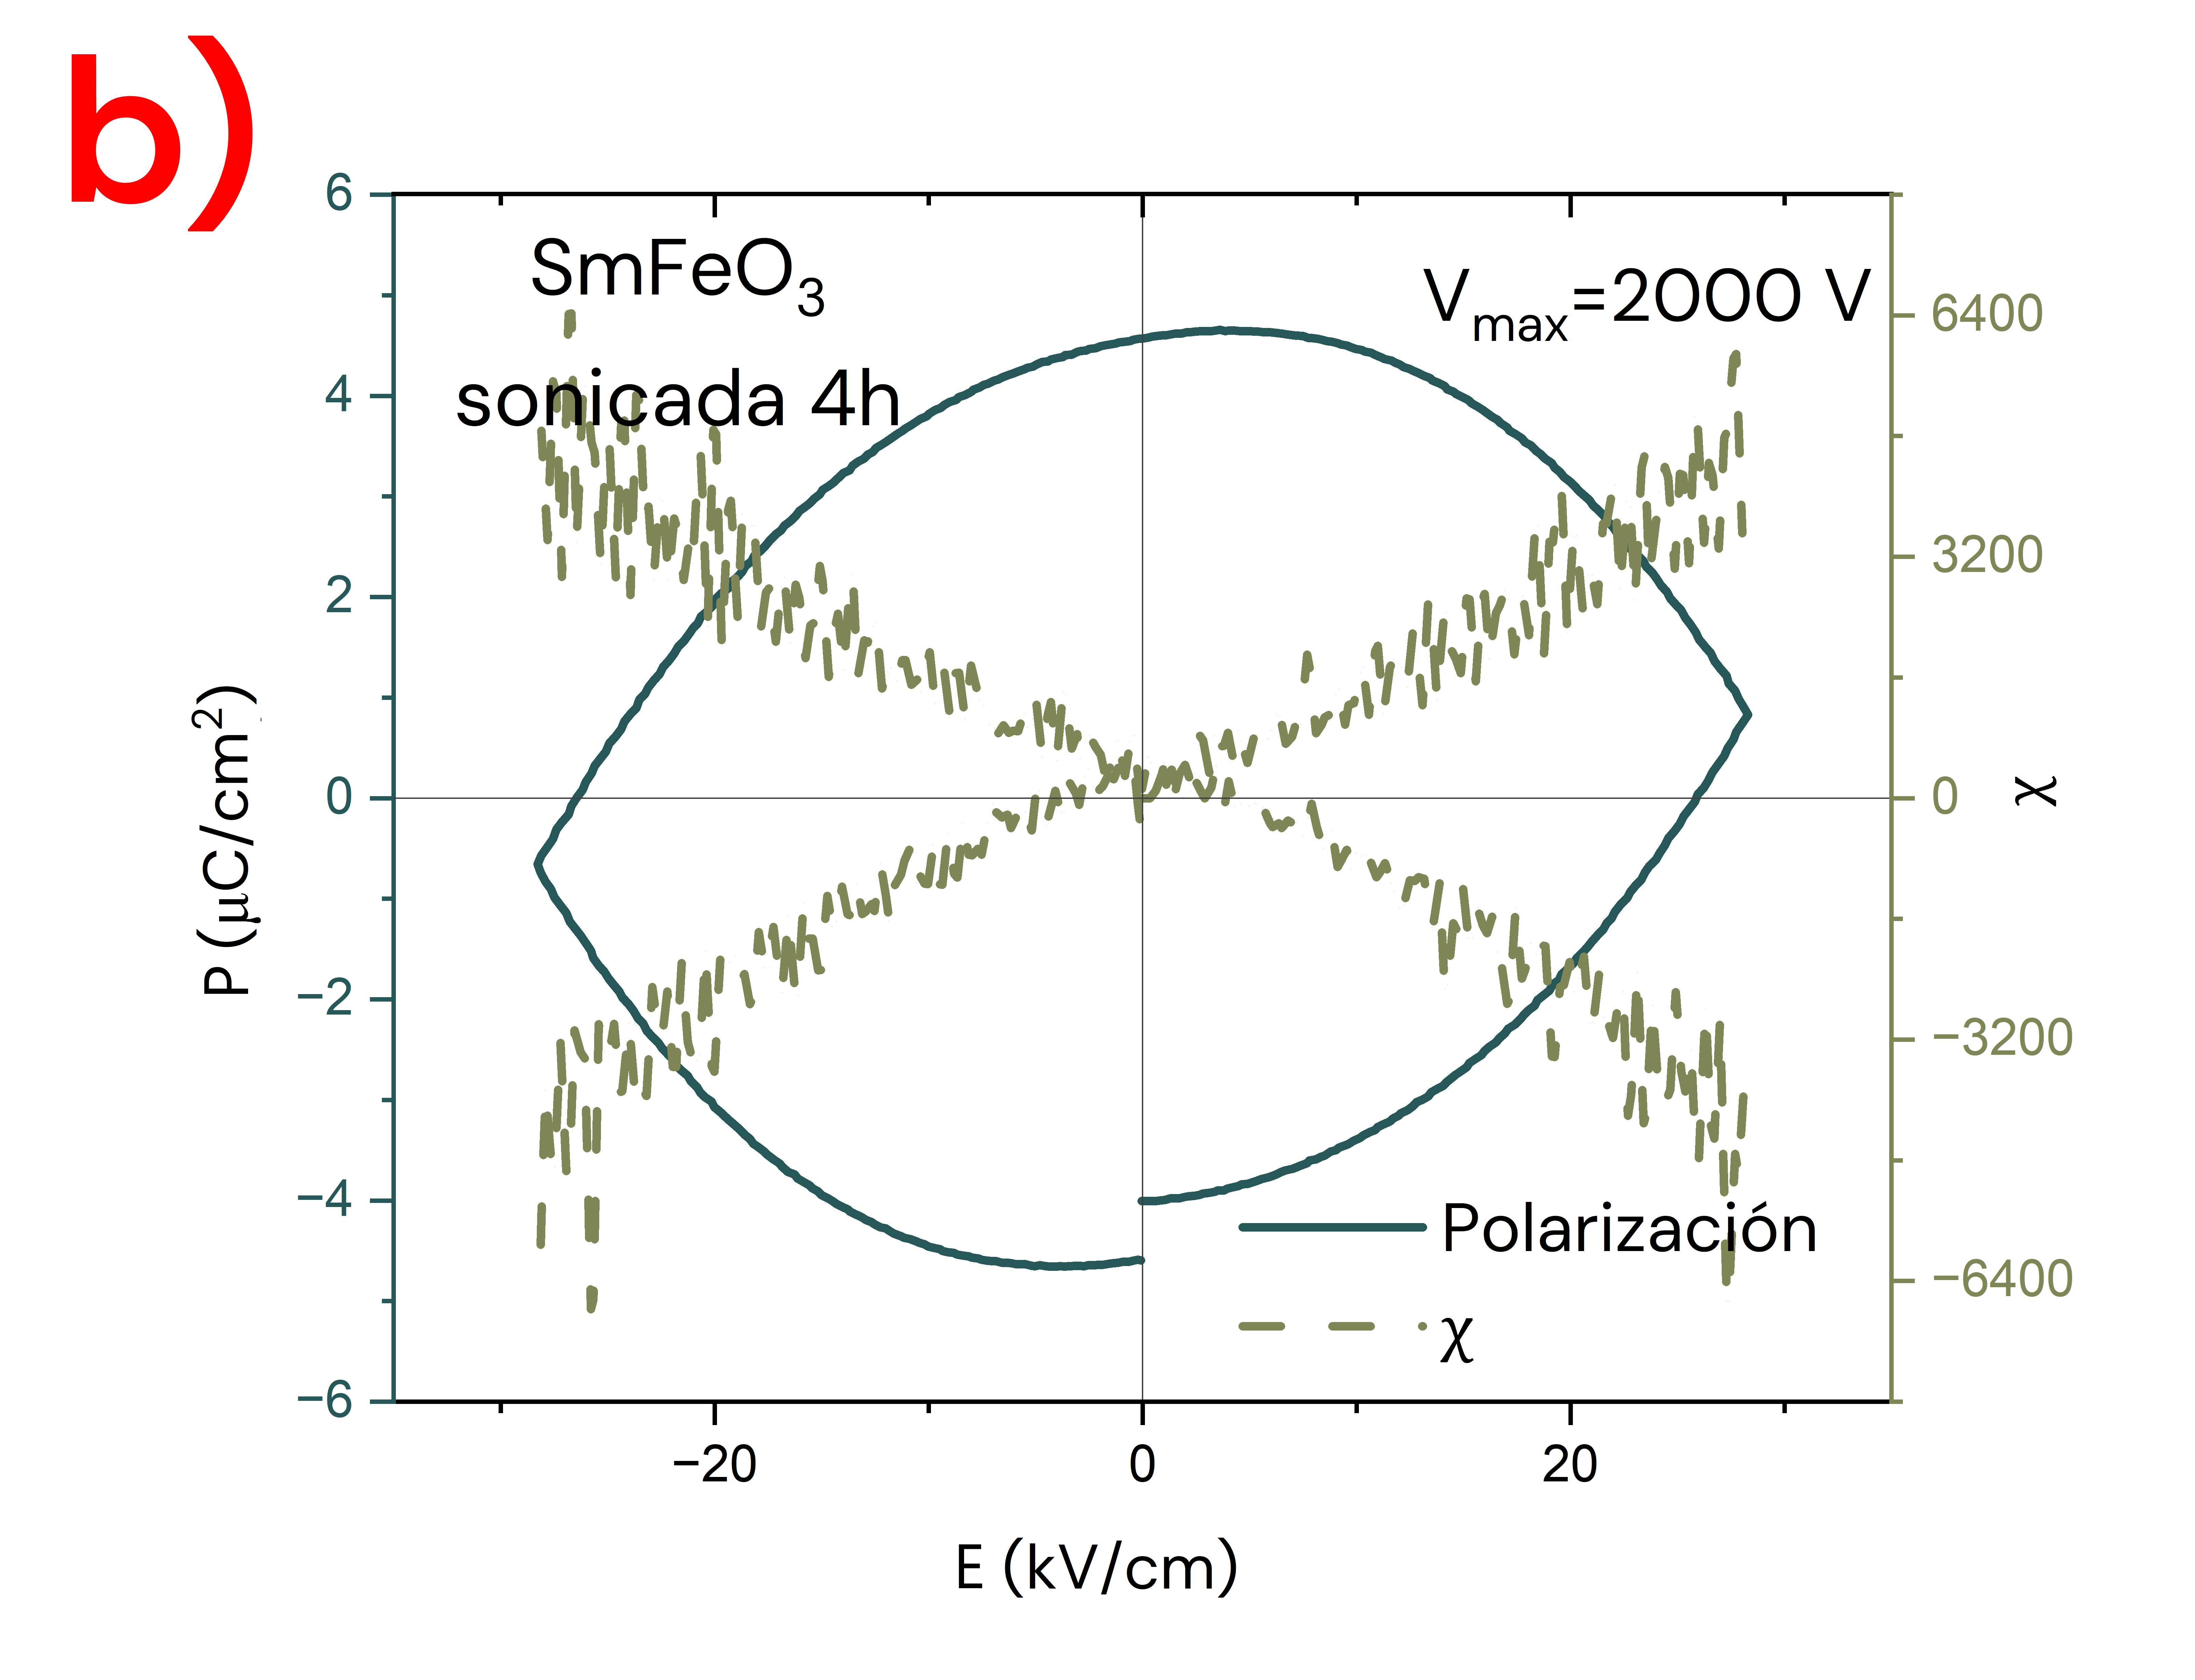
\includegraphics[width=0.45\textwidth]{fig/PESmFeO3-S2000V.png}
    \caption{Curvas $P$ contra $E$ (eje izquierdo) y $\chi$ contra $E$ (eje derecho) con $V_\text{max}=2000$ V de las muestras de \sama{}: a) sin sonicar y b) sonicada 4 h.}
    \label{fig:sm2000v}
\end{figure}
De forma similar a las muestras de \neod{} se observa un comportamiento de histéresis débil a $V_\text{max}=100$ V (figuras \ref{fig:sm100v} a) y b)), sin embargo, este no se pierde completamente al subir el voltaje para la muestra de \sama{} sin sonicar (figura \ref{fig:sm2000v} a)).

A continuación se reportan los valores obtenidos para $P_r$, $P_s$ y $E_c$ para las mediciones con $V_\text{max}=100$ V.

\begin{table}[H]
    \centering
    \begin{tabular}{|c||c|c|c|}
        \hline
        Muestra & $P_s$ ($\mu$C/cm$^2$) & $P_r$ ($\mu$C/cm$^2$) & $E_c$ (kV/cm) \\
        \hline\hline
        \sama{} sin sonicar & 0.0072 $\pm$ 0.00032 & $0.0022 \pm 0.00062$ & $0.3794 \pm 0.04913$ \\
        \hline
        \sama{} sonicada & 0.0054 $\pm$ 0.00018 & $0.0037 \pm 0.00011$ & $0.7354 \pm 0.05652$ \\
        \hline
        \end{tabular} 
        \caption{Valores de $P_r$, $P_s$ y $E_c$ medidos de las muestras de \sama{} sin sonicar y sonicada 4 h.}
    \label{tabla:respolarsama}
\end{table}
De igual forma se observan valores pequeños de $P_s$, $P_r$ y $E_c$ para todas las muestras. La sonicación no tuvo un efecto notorio en las propiedades eléctricas.
\end{document}